\documentclass[sommairechap,stylejchiquet]{these_gi}



\begin{document}

% ==================================================================
% OPTIONS D'AFFICHAGE
% non-d�finitif (soumis aux rapporteurs) ou  d�finitif
\definitiftrue
% \definitiffalse

% ==================================================================
% RENSEIGNEMENTS SUR LA TH�SE
\titleFR{D�codage des intentions et des repr�sentations motrices chez l'homme: analyse multi-�chelle et application aux interfaces cerveau-machine}
\titleEN{Le titre en anglais}
\abstractFR{Le r�sum� en fran�ais ($\approx$ 1000 caract�res)}
\abstractEN{Le r�sum� en anglais ($\approx$ 1000 caract�res)}
\keywordsFR{Les mots-cl�s en fran�ais}
\keywordsEN{Les mots-cl�s en anglais}
 
\author{Etienne Combrisson}
\address{e.combrisson@gmail.com}
\universite{universit� claude bernard lyon 1}
\laboratoire{}
\specialite{sp�cialit� de la th�se}
\datesoutenance{09/2016}
\datesoumission{la date de soumission aux rapporteurs}
\jury{\begin{tabular}{llll}
    M\up{me} & \textsc{Erika Rat�} & Universit� � la Menthe & (Rapporteur) \\
    M. & \textsc{Jacques Ouille} & Universit� � la Fraise & (Rapporteur) \\
    M. & \textsc{Henri Zoto} & Laboratoire laborieux & (Rapporteur) \\
    M. & \textsc{Jean File} & Indienne & (Directeur) \\
       & etc. &  \\
  \end{tabular}    
}
{
% ==================================================================
% D�DICACE
\dedicate{� Isabelle et Didier, mes deux parents,\\ qui ont tout donn� pour que ceci me soit un jour possible. \\ Merci}
 
% ==================================================================
% DEBUT DE LA PR�FACE
\beforepreface
 
% ==================================================================
% COUVERTURE : RESUME ET MOTS-CL�S
\abstractpage
 
% remerciements
\chapter*{Remerciements}

%% Encadrant
\malettrine{J}{e}  voudrais tout  d'abord exprimer  mes  plus profonds
remerciements �\dots AH���H !

% �lo�se
Je conclurai en  remerciant de tout c{\oe}ur (l'�tre aim�).

\vspace{2cm}

\hfill Montr�al, le \today.


 
% table des mati�res g�n�rale
{
\hypersetup{linkcolor=black}
\tableofcontents

 
% affiche la liste des figures
\newpage
\listoffigures
}
% ==================================================================
\afterpreface

% ==================================================================
% NOTATIONS
\chapter*{Notations}
\addcontentsline{toc}{chapter}{Notations}

\pagestyle{plain}

%----------------------------------
% GENERAL
%----------------------------------
\Large G\'en\'eral \\% \bigskip
\normalsize
\begin{supertabular}{ll}
  ICM & Interface Cerveau-Machine \\
  BCI & Brain Computer Interface \\
\end{supertabular}

%----------------------------------
% ENREGISTREMENTS
%----------------------------------
\vspace{1cm}
\Large Enregistrements \\% \bigskip
\normalsize
\begin{supertabular}{ll}
  EEG & \eeg \\
  MEG & \meg \\
  SUA & \sua \\
  MUA & \mua \\
  SEEG & \seeg \\
  ECoG & \ecog \\
\end{supertabular}

%----------------------------------
% FEATURES
%----------------------------------
\vspace{1cm}
\Large Features \\% \bigskip
\normalsize
\begin{supertabular}{ll}
  PAC & Phase Amplitude Coupling \\
\end{supertabular}

%----------------------------------
% CLASSIFIEURS
%----------------------------------
\vspace{1cm}
\Large Classifieurs \\% \bigskip
\normalsize
\begin{supertabular}{ll}
  LDA & \lda \\
  SVM & \svm \\
  RF & \rf \\
  KNN & \knn \\
  NB & \nb \\
\end{supertabular}

\chapterend

% ==================================================================
% AVANT-PROPOS
% *****************************************************************************
% *****************************************************************************
%                                   INTRODUCTION
% *****************************************************************************
% *****************************************************************************
\part{Introduction}
\pagestyle{headings}

\chapter*{Probl�matique}

L'objectif principal de cette th�se est d'utiliser les outils de d'apprentissage machine (ou \textit{machine-learning}) pour extraire des marqueurs de l'activit� neuronale, un marqueur �tant un motif qui appara�t de mani�re robuste et syst�matique lorsque la t�che se r�p�te. L'approche traditionnelle d'analyse, dite \textit{hypothesis-driven}, consiste � formuler une hypoth�se cibl�e en amont qui est ensuite confirm�e ou rejet�e par les r�sultats des analyses. L'approche de cette th�se s'inscrit dans une d�marche r�cente en neuroscience et consiste en une exploration dite \textit{data-driven}. Cette approche, qui est devenue envisageable gr�ce aux progr�s informatique, permet une investigation plus large et plus ensembliste dont la strat�gie est dict�e par les donn�es. \\
Cette m�thodologie d'apprentissage machine a souvent �t� utilis�e sur des donn�es c�r�brales dans le contexte des \icm (ICM). Dans un premier temps, la machine apprend � reconna�tre des motifs, ou \textit{pattern} associ�s � un �tat cognitif particulier puis, dans un second temps, les motifs reconnus sont transcrits en commandes. Ces approches sont particuli�rement prometteuses mais leur acuit� d�pend grandement du choix des attributs c�r�braux. En cons�quence, pour am�liorer ces approches il faut am�liorer le choix des marqueurs et donc, am�liorer notre connaissance des corr�lats neuronaux li�s aux processus moteur. Cette exploration de la pertinence de divers attributs oscillatoires propres aux intentions motrices repr�sentent justement ce que nous proposons d'entreprendre dans ce travail de th�se. Ainsi, les outils de \textit{machine-learning} ont �t� employ�s pour identifier les m�canismes les plus pertinents et permettant de pr�dire \textit{(a)} les �tats moteurs et \textit{(b)}, les directions de mouvement, que ce soit durant son ex�cution ou sa pr�paration. \\
L'approche \textit{data-driven} permet certes une investigation � grande �chelle mais requi�re en cons�quence des outils efficaces pour un temps d'ex�cution raisonnable et d'autre part, des outils adapt�s aux formats des donn�es neuroscientifiques. Dans ce cadre, une partie importante de cette th�se a �t� d�di� � la mise en place d'outils informatiques permettant d'analyser et de visualiser les r�sultats d'analyses. Ces outils logiciels d�velopp�s en Python constituent en soi une contribution m�thodologique significative de cette th�se. Ces paquets \textit{open-source} � la disposition de la communaut� scientifiques sont au nombre de trois et comptabilisent $52533$ lignes de code pures, plus de $90000$ en incluant leurs documentations respectives disponible en ligne. L'int�gralit� des analyses et des figures pr�sent�s durant cette th�se sont issus des logiciels que nous avons impl�ment�. \\
En introduction nous poserons le cadre li� au d�codage de l'activit� neuronale et aux m�canismes c�r�braux impliqu�s dans les processus moteurs. Puis nous pr�senterons les m�thodologies associ�es ainsi que les solutions informatiques mises en place. Puis nous pr�senterons un premier article m�thodologique en \textit{machine-learning} (Article 1 (\ref{seuil_chance})), deux articles sur le d�codage des intentions motrices � partir de donn�es intrac�r�brales (Article 2 (\ref{Etude2_encodage}) et 3 (\ref{Etude3_decodage})) et pour finir, trois articles qui pr�sentent les d�veloppements logiciels (Articles 4 (\ref{Etude4_tensorpac}), 5 (\ref{Etude5_visbrain}), 6 (\ref{Etude6_sleep})).

% #############################################################################
%                                CORPS DE L'INTRO
% #############################################################################
% #############################################################################
%                      Classification des signaux c�r�breaux
% #############################################################################
\chapter{D�codage de l'activit� c�r�brale}


% -----------------------------------------------------------------------------
% -----------------------------------------------------------------------------
%                            DEFINITION D UNE ICM
% -----------------------------------------------------------------------------
% -----------------------------------------------------------------------------
\section{Les \icm}

\subsection{D�finition et objectifs}
Cette premi�re section a pour but d'introduire et de d�finir le concept d'\icm. Nous verrons dans quel contexte elles sont apparues, les personnes � qui elles sont destin�es ainsi que les principaux �l�ments qui les composent. \\
Point de vue lexicale, on utilisera indiff�remment \textit{Interface Cerveau-Machine (ICM)}, \textit{Interface Cerveau-Ordinateur (ICO)} ou les termes anglais correspondant � savoir \textit{Brain Computer Interface (BCI)} et \textit{Brain Machine Interface (BMI)}.

% ********************************************
%           CONTEXTE D'APPARITION
% ********************************************
\subsubsection{Contexte d'apparition des ICM}
En 1964, Dr. Grey Walter connecte des �lectrodes directement dans le cortex moteur d'un patient et lui demande de presser un bouton pour faire avancer un r�tro-projecteur. En m�me temps, il enregistre l'activit� neuronale de telle sorte que elle aussi, puisse le faire avancer. L� o� l'exp�rience devient remarquable, c'est que le r�tro-projecteur avance avant que le patient ne presse le bouton ! Tout l'appareil musculaire du sujet est court-circuit� et le contr�le se fait sans mouvement. Contr�ler par la \textit{pens�e}, un sujet de science fiction qui devient une r�alit�. Cette anecdote d�crite par \cite{graimann_braincomputer_2009}, permet de placer la naissance de la possibilit� d'une \icm (ICM) dans l'histoire. C'est le point d'entr�e qui a ensuite conduit une grande diversit� de chercheurs � se passionner pour ce sujet. \\
Le terme \textit{Brain Computer Interface} fait son apparition, au d�but des ann�es 70, dans les publications de Jacques Vidal \citep{vidal_toward_1973, vidal1977real} o� il �tait question de contr�ler un curseur sur un �cran. \\
La progression des ICM et de l'int�r�t de la communaut� scientifique � v�ritablement commenc� dans les ann�es 2000. Trois facteurs sont � l'origine \citep{wolpaw_brain_2002}:
\begin{enumerate}
	\item Une am�lioration des connaissances des processus neuro-physiologiques et des techniques d'imagerie.
	\item L'arriv�e d'ordinateur bon march� et l'am�lioration constante de leur performances et des composants �lectroniques (processeurs, m�moire vive, logiciel...)
	\item Une prise de conscience soci�tale des besoins de personnes souffrant de probl�mes neuro-musculaires.
\end{enumerate}
A noter que, � l'heure actuelle, l'arriv�e de cartes graphiques bon march� est entrain de r�volutionner l'approche computationnelle des ICM permettant des calculs plus lourds en moins de temps (notamment pour le \textit{Deep Learning}). Outre la continuelle am�lioration des composants et de leur miniaturisation, la prochaine r�volution concernera certainement les ordinateurs quantiques, d�j� en phase de test dans les domaines de la g�n�tique et de la chimie. 

% ********************************************
%               INTERACTIONS NATURELLES
% ********************************************
\subsubsection{Interactions naturelles avec l'environnement}
Pour interagir avec son environnement, l'individu se sert des voies de communications naturelles, \cad via son syst�me nerveux et musculaire. Le processus de communication d�bute par une intention qui active certaines r�gions dans le cerveau. Il en r�sulte un signal c�r�brale qui est ensuite envoy� par le syst�me nerveux p�riph�rique en directions des muscles \citep{besserve_analyse_2007}. C'est ce processus simplifi� qui permet � une personne d'interagir avec ce qui l'entoure.

% ********************************************
%           COMMUNICATION ALTERNATIVE
% ********************************************
\subsubsection{Un canal de communication alternatif}
Il existe plusieurs maladies ou accidents qui entra�nent une d�g�n�rescence des performances motrices. Parmi elles, ont peut par exemple citer la Scl�rose Lat�rale Amyotrophique (ou SLA), les accidents vasculaires c�r�braux, certaines formes de scl�rose, les l�sions de la moelle �pini�re... Toutes ont en commun la possibilit� de probl�me moteur. Dans ce contexte, \cite{wolpaw_brain_2002} introduit trois options pour restaurer ces fonctions:
\begin{enumerate}
	\item Augmenter les capacit�s des facult�s motrices restantes. Autrement dit, donner un sens nouveau aux mouvements que l'individu est toujours en capacit� de faire. A titre d'exemple, le guitariste virtuose Jason Becker, reconnu pour sa v�locit� et dont tout le monde s'entendait sur son incroyable talent, f�t un jour frapp� par la SLA le conduisant au fur et � mesure � l'immobilit� totale. Il convenu alors d'un langage bas� sur les mouvements oculaires et, avec la complicit� de son p�re, continua de composer.  
	\item Contourner la l�sion. L'auteur donne � titre d'exemple, une l�sion de la moelle �pini�re que l'on peut contourner en utilisant l'activit� des muscles situ�s au dessus de la l�sion pour stimuler les muscles paralys�s.
	\item Enfin, la derni�re fa�on de restaurer des fonctions motrices qui prend tout son sens lorsque les deux pr�c�dentes ne sont pas possibles, c'est d'�tablir un nouveau canal de communication directe entre le cerveau et un ordinateur, et ce, ind�pendamment de l'activit� musculaire. D'o� le nom, \textit{\icm}.
\end{enumerate}
Une ICM est un autre syst�me de communication o� les voies naturelles sont cout-circuit�es. Au lieu de passer par le syst�me nerveux puis musculaire, le signal c�r�bral est directement intercept� au niveau du cerveau et va ensuite �tre transform� en commandes. Une ICM est donc un syst�me permettant de traduire une activit� neuronale en commande ext�rieure. Le terme \textit{traduire} est � prendre au sens linguistique \cad que les signaux c�r�braux forment un langage, compos� de r�gles, de motifs ou \textit{pattern}, que l'on va essay� de d�coder (via un ordinateur) pour les transformer en op�rations. D'o� le terme "\icm". \\

\cite{pfurtscheller_rehabilitation_2008} et \citep{graimann_braincomputer_2009} introduisent quatre �l�ments qui composent une ICM:
\begin{enumerate}
	\item Enregistrer l'activit� directement depuis le cerveau. Cet enregistrement pourra �tre invasif ou non-invasif (cf. \ref{invasif_non-invasif})
	\item G�n�rer un retour ou \textit{feedback} pour l'utilisateur
	\item L'enregistrement et le \textit{feedback} doivent �tre en temps r�el
	\item Enfin, l'interface doit �tre contr�lable par l'utilisateur, de mani�re active, via un ensemble d'intentions. 
\end{enumerate}
A titre d'exemple et pour illustrer ce dernier point, un utilisateur pourrait par exemple d�cider de bouger un curseur de souris sur un �cran en imaginant des mouvements soit de la main gauche soit de la main droite.


% ********************************************
%         COMPOSANTES D'UNE ICM
% ********************************************
\subsubsection{Principales composantes d'une ICM}
M�me si chaque \icm se destine � une utilisation particuli�re et contient des traitements qui lui sont propres, on peut globalement dire qu'une ICM s'articule autour de cinq grandes �tapes ordonn�es \citep{pfurtscheller_rehabilitation_2008,graimann_braincomputer_2009}:
\begin{enumerate}
	\item L'acquisition de l'activit� neuronale
	\item Les pr�-traitements
	\item L'extraction de marqueurs
	\item La classification
	\item La transformation en commande
\end{enumerate}
Ces �tapes sont interd�pendantes \cad que chacune s'appuie sur les r�sultats de l'�tape pr�c�dente. De plus, cette cascade de stades doit se faire en temps r�el pour que l'exp�rience utilisateur soit la plus fluide possible et qu'elle refl�te fid�lement ce qui se d�roule � chaque instant.

% -> Acquisition de l'activit� neuronale :
\paragraph{Acquisition de l'activit� neuronale}
L'acquisition de l'activit� neuronale constitue le point d'entr�e d'une ICM. Les diff�rentes techniques pour enregistrer sont plus ou moins accessibles (certaines sont portatives, d'autres n�cessitent un appareil tr�s lourd...). C'est, entre autre, l'accessibilit� qui va influer sur le nombre de sujets d'une �tude. Autre point tr�s important que nous d�crirons plus bas, la qualit� du signal (ou le rapport signal sur bruit (RSB)) qui aura un impact imm�diat sur les performances et sur les limitations d'une ICM. Enfin, on parlera d'enregistrements \textit{invasifs} (cf. \ref{sec_invasif_recordings}) quand ceux-ci n�cessiteront une implantation chirurgicale d'�lectrodes et \textit{non-invasif} (cf. \ref{sec_noninvasif_recordings}) pour les techniques d'acquisition se faisant en dehors de la bo�te cr�nienne.

% -> Pr�-traitements :
\paragraph{Pr�-traitements}
Les pr�-traitements regroupent un ensemble de techniques destin�es � nettoyer le signal pour faire ressortir, autant que possible, le signal utile par rapport au signal bruit�. Parmi ces traitements, on peut citer le nettoyage d'artefacts oculaires, cardiaques ou musculaires, le r�f�rencement (essentiellement pour l'EEG), la bipolarisation (pour la SEEG), le filtrage pour supprimer certaines composantes spectrales... Ces pr�-traitements sont propres � chaque technique d'enregistrement. Une description plus d�taill�e des pr�-traitements appliqu�s dans le cadre de donn�es SEEG est propos�e dans la section \ref{SEEG_preprocessing}.

% -> Extraction des marqueurs :
\paragraph{Extractions de marqueurs}
\label{subsec_marqueurs_ICM}
En imaginant que l'on r�p�te dix fois le m�me mouvement, il y aura dans l'activit� neuronale une partie similaire permettant de reproduire chacune de ces r�p�titions. Le signal entier sera tr�s probablement diff�rent � chaque fois, mais, � l'int�rieur de ce signal, on pourra trouver un "sous-signal" dont le contenu sera similaire � chacune de ces r�p�titions. \\
C'est le but de cette �tape d'extraction de marqueurs, la recherche de ce "sous-signal". Une fois l'activit� c�r�brale nettoy�e, on va chercher � extraire des marqueurs qui mat�rialisent l'�tat instantan� d'un sujet. Par exemple, si celui-ci bouge le bras vers la gauche ou vers la droite, on doit pouvoir extraire une information de ce signal qui encode chacun de ces �tats. En pratique, on peut distinguer deux types de marqueurs: les marqueurs \textit{locaux}, qui refl�tent l'activit� d'une "petite" population de neurones prises localement (cf. \ref{sec_marqueurs_AN}), et les marqueurs d'\textit{interaction} qui quantifie un degr�s de couplage � distance entre deux r�gions du cerveau. \\
Cette �tape est v�ritablement au c\oe ur du bon fonctionnement d'une ICM puisque, en fonction de la qualit� de ce marqueur, la machine sera plus moins encline � reconna�tre les diff�rentes commandes d'un sujet. \\    
En lieu et place du terme \textit{marqueur}, on pourra utiliser indiff�remment \textit{motif}, \textit{pattern}, \textit{feature} ou \textit{attribut}.  

% -> Classification :
\paragraph{Classification}
En reprenant l'exemple de la section pr�c�dente, supposons que l'on dispose d'un marqueur et on cherche � savoir si celui-ci appartient � une des deux classes de mouvement de bras, vers la gauche ou vers la droite. C'est le probl�me de classification. A partir d'un motif dont on ignore la provenance, on utilise un algorithme permettant de reconna�tre la classe dont est issue ce pattern. Parmi les algorithmes les plus fr�quemment rencontr�s, on peut citer le \lda, le \svm ou le \knn.\\
En pratique, cette reconnaissance de classes est mise en place en deux �tapes:
\begin{enumerate}
	\item L'entra�nement ( ou \train): durant une certaine p�riode, on va apprendre � une machine � reconna�tre des �v�nements. Pour cela, on utilise des donn�es dont on conna�t la provenance (c'est ce que l'on appelle la \textit{labellisation})
	\item Le test ( ou \test): une fois la machine entra�n�e � partir d'une s�rie de marqueurs lab�lis�s, on teste l'algorithme avec des nouvelles donn�es pour �valuer l'acuit� de la machine � identifier ces �v�nements.
\end{enumerate}
Quelque soit l'algorithme de classification, celui-ci doit s'adapter � chaque utilisateur suivant trois niveaux \citep{wolpaw_brain_2002}:
\begin{enumerate}
	\item En premier lieu, et de mani�re assez �vidente, il doit pouvoir s'adapter au marqueur du sujet
	\item Ensuite, l'algorithme doit s'adapter en temps-r�el aux variations spontan�es. En effet, l'exp�rience utilisateur va varier en fonction d'un certain nombre de param�tres comme le moment de la journ�e, la fatigue, la maladie, le taux d'hormones, la motivation/concentration/frustration... \citep{curran_learning_2003}
	\item Enfin, il doit permettre de prendre en compte l'adaptation du sujet. Durant l'exp�rience, l'utilisateur module son activit� et fournit des efforts pour s'adapter au fonctionnement de la machine. En contrepartie, le software doit prendre en compte cette am�lioration en fournissant des performances accrues.
\end{enumerate}
Cette �tape de classification, d�crite plus largement dans la section \ref{methodo_classification}, est tr�s fortement d�pendante de la qualit� des marqueurs extraits en amont. Autrement dit, plus ces \textit{features} refl�tent fid�lement un �tat, plus le travail de la machine � identifier ces �v�nements sera facilit�.

% -> Commande :
\paragraph{Transformation en commande}
Derni�re �tape du processus d'une ICM, lorsque l'algorithme de classification pense avoir identifier le type de marqueurs, on attribue une commande physique. Par exemple, si la machine reconna�t un mouvement de bras vers la droite, on pourrait attribuer une commande o� l'on d�place le curseur d'une souris sur un �cran dans la m�me direction. Ainsi, on procure � l'utilisateur un \textit{feedback} sur la transformation que la machine a r�ussit � faire � partir de l'activit� de son cerveau.\\
Cette transformation en commande est ensuite physiquement appliqu�e � un syst�me externe. L'efficacit� de l'ensemble de l'ICM est donc �valu�e en fonction de son acuit� � restituer, avec plus ou moins de fid�lit�, la commande d�sir�e par l'utilisateur.

\figScaleDesciption{0.7}{Pfurtscheller2008_SchemaICM}{Sch�ma d'une \icm \citep{pfurtscheller_rehabilitation_2008}}{L'activit� neuronale est enregistr�e (Signal acquisition) puis nettoy�e (Preprocessing). Ensuite, on extrait des motifs ou patterns qui caract�risent la commande que souhaite envoyer le sujet (Feature extraction). Enfin, la machine tente de reconna�tre ces motifs (Classification) et de les transformer en commande (Application interface). Cette boucle se termine en donnant un feedback � l'utilisateur sur l'�tat actuel de la machine. \citep{pfurtscheller_rehabilitation_2008}}

Les ICM partagent globalement ces cinq �tapes mais se diff�rencient donc le type d'enregistrement de l'activit� neuronale, par les pr�-traitements associ�s, par le type de marqueurs �tudi�, par l'algorithme de classification choisi et surtout, par l'application concr�te de cette \icm.

% ********************************************
%           Applications des ICMs
% ********************************************
\subsubsection{Applications des ICM: cliniques et non-cliniques}
La r�alisation concr�te des ICM s'est articul�e autour des applications cliniques, \cad destin�es � essayer d'am�liorer les conditions de vie de certaines personnes puis, dans un second temps, pour des applications ludiques et tout publique.

\paragraph{Applications cliniques}
A l'heure actuelle, il existe de nombreuses maladies soit dont on ignore l'origine, soit qui sont pour le moment incurables. Parmi ces pathologies, certaines �voluent en enfermant les patients dans des conditions de vies difficiles. C'est dans ce contexte clinique qu'apparaissent de nombreuses ICM qui ne sont donc pas des traitements, mais bien des solutions \textit{temporaires} pour aider certaines personnes � mieux vivre avec leur handicap.
\subparagraph{Pathologies et ICM :} Pr�lever directement l'activit� neuronale et donc, \textit{bypasser} les voies naturelles, permet de s'affranchir d'�ventuelles limitations physiologiques. C'est pourquoi les ICM repr�sentent un enjeu majeur pour la r�habilitation motrice ou handicap moteur ou encore pour la communication palliative. Les applications concr�tes des \icm visent donc les personnes disposant de leurs capacit�s cognitives mais qui sont priv�es de facult�s motrices. \\
Un accident vasculaire c�r�brale (AVC) peut engendrer un �tat d'enfermement (\textit{locked-in state (LIS)}). Les personnes dans cet �tat sont pleinement conscientes de leur corps, de l'environnement, ils peuvent ressentir les sensations de toucher et de douleur mais n'ont plus de facult�s motrices, hormis peut-�tre, les mouvements de paupi�res ou des yeux. Un autre exemple est celui de la scl�rose lat�rale amyotrophique (ou SLA) qui est une d�g�n�rescence des neurones moteur (motoneurones). Progressivement, les personnes atteintes de SLA perdent l'usage des bras, des jambes, de la parole des muscles faciaux et enfin de la d�glutition mais la conscience et les facult�s cognitives demeurent intactes. L'�volution de la maladie am�ne � deux possibilit�s \citep{chaudhary_brain-machine_2015}: accepter une d�pendance totale (respiration artificielle et nutrition) ou un d�c�s par insuffisance respiratoire. Dans le premier cas, la maladie entra�ne progressivement les patients en LIS ne leur laissant qu'un minimum de fonctions motrices. Lorsque le patient perd tout contr�le musculaire, ce qui finit souvent par les muscles des yeux, il rentre dans un �tat d'enfermement complet (\textit{completely locked-in state (CLIS)}). \\
SLA et \textit{locked-in syndrome} ne sont que deux exemples expliquant l'int�r�t social du d�veloppement des ICM. Redonner un peu de contr�le ou �tablir un canal de communication avec les familles des patients expliquent l'engouement qui existe depuis maintenant plus de 40 ans pour les ICM.

\figScaleDesciption{0.5}{SLA_physio2}{Paralysie caus�e par la SLA et accident vasculaire c�r�brale \citep{kubler2001brain}}{Paralysie caus�e par la SLA et accident vasculaire c�r�brale \citep{kubler2001brain}}

\textbf{Exemples d'applications:} les applications cliniques peuvent �tre divis�es en deux grandes familles: les ICM destin�es � r�tablir un lien de communication (\textit{communication palliative}) et les ICM pour redonner de la mobilit�. \\

\textbf{Communication palliative:} ces ICM pr�sentent en g�n�ral des lettres ou groupe de lettres qui doivent pouvoir �tre s�lectionn�s volontairement par l'utilisateur. Le \textit{P300-Speller} \citep{farwell_talking_1988, donchin_mental_2000}, utilisant l'onde P300, est sans aucun doute l'interface la plus connue et la plus exploit�e � ce jour pour la communication palliative. Le \textit{Hex-o-spell} \citep{blankertz_note_2007} est une autre interface contr�lable par l'utilisateur via l'imagerie motrice. \\

\textbf{Mobilit�, robotique et proth�se:} ces syst�mes sont destin�s � aider, am�liorer ou remplacer des facult�s motrices l�s�es. Ces applications dont la mobilit� est au centre peuvent afficher diff�rents degr�s de complexit�:
\begin{itemize}
	\item Curseur $1D$, $2D$ et $3D$: certainement la premi�re �tape, le but ici est de permettre au sujet de pouvoir contr�ler le curseur sur un moniteur. Ce curseur pourra par exemple servir de bouton \textit{yes/no} ou pour le d�placement \citep{wolpaw1991eeg, wu_neural_2003, trejo2006brain, kayagil2009binary, sung-phil_kim_point-and-click_2011, vadera_stereoelectroencephalography_2013} ou tout simplement pour de la navigation comme le \textit{web-browsing} \citep{mugler_design_2010}. Ces cat�gories de d�placement de curseur diff�rent par le nombre de degr�s de libert� qu'elles offrent.  
	\item Contr�le d'un fauteuil roulant: comme le nom l'indique, l'id�e ici est de permettre � un utilisateur de contr�ler son fauteuil roulant via son activit� neuronale seulement. En effet, si de nombreuses personnes handicap�es peuvent encore se servir de leur membres sup�rieurs, d'autres sont compl�tement d�pendantes. Ce type d'applications permettra donc � terme de redonner une lib�rt� de mouvement � ces personnes \citep{tanaka2005electroencephalogram, leeb_self-paced_2007, galan_brain-actuated_2008, philips_adaptive_2007, vanacker_context-based_2007, pires_visual_2008, rebsamen_brain_2009, lin_eeg_2010, diez_commanding_2013}.
	\item Proth�se: enfin, derni�re application li�e � la mobilit�, le contr�le de proth�se est un large d�fi. A titre d'exemple, le contr�le d'un bras robotis� doit permettre le contr�le de celui-ci dans l'espace ainsi que des mouvements de main, de coude... C'est un probl�me � haute dimensionnalit� et donc complexe. Toutefois, modulo un certain degr�s de r�ussite, certaine �quipe ont propos� de tel syst�mes \citep{fetz_real-time_1999, hochberg_reach_2012, yanagisawa_electrocorticographic_2012, sunny_robotic_2016}
\end{itemize}

\paragraph{Applications non-cliniques et r�cr�atives}
Les ICM ont �galement �t� exploit�es � d'autres fins que des applications cliniques:
\subparagraph{Jeux:} les ICM d�di�es aux jeux utilisent l'activit� neuronale pour contr�ler un vaisseau spatial, un objet ou un personnage dans un environnent virtuel \citep{lalor_brain_2004, nijholt_bci_2008, oude_bos_brainbasher_2008, coyle_eeg-based_2011}. Outre le caract�re r�cr�atif de ce type de dispositif, les ICM bas�es sur le jeux pourraient tr�s bien servir pour entra�ner la machine d'une mani�re plus ludique et moins fatigante.
\subparagraph{Art:} pour finir, les ICM peuvent avoir des applications artistiques comme pour la composition et la pratique musicale \citep{miranda_harnessing_2003, miranda_brain-computer_2006, hamadicharef_brain-computer_2010} ou pour peindre \citep{munsinger_brain_2010, zickler2013brain}

% ********************************************
%                 OPEN DATA
% ********************************************
\subsubsection{\textit{BCI competition} et \textit{open-data}}
Les \textit{BCI competitions} sont propos�es par l'�quipe du \textit{Berlin Brain-Computer Interface} (BBCI). L'id�e de ces comp�titions est, sur un m�me jeux de donn�es d�coup�es en \train et \test (cf. \ref{subsec_training_testing}) mettre les �quipes de recherche en ICM en comp�titions puis �lire celle qui arrivera au meilleur d�codage. A l'heure o� cette th�se est �crite, quatre de ces comp�titions ont eut lieu et chacune est associ�e � un article de pr�sentation (\textit{BCI competition I}: \cite{sajda_data_2003}, \textit{II}: \cite{blankertz_bci_2004}, \textit{III}: \cite{blankertz_bci_2006}, \textit{IV}: \cite{tangermann_review_2012}). La liste des \textit{datasets} en acc�s libres est disponible en annexe (cf. \ref{annexe_bci_competition}. Remarque: il semble que les donn�es de la premi�re comp�tition ne soient plus accessibles, c'est la raison pour laquelle elles n'apparaissent pas dans le tableau)\\

Ces comp�titions pr�sentent de nombreux avantages:
\begin{enumerate}
	\item Visibilit� des �quipes: ces comp�titions sont de plus en plus "virales" et sont relay�es par la suite par de nombreux articles (voir figure ci-dessous). 
	\item Permet aux �quipes de disposant pas de syst�mes d'acquisition de profiter de jeux de donn�es pour d�velopper des m�thodes. C'est �galement un moyen d'initier les �tudiants � un ensemble de techniques.
	\item Autre avantage, tout le monde se retrouve sur un pied d'�galit� en travaillant sur les m�mes donn�es. Ce qui repr�sente par la suite, une m�thode rigoureuse pour s�lectionner les meilleurs algorithmes.
\end{enumerate}

\figScaleDesciption{1}{bcicomp_visi}{\textit{BCI competition} et visibilit� \cite{tangermann_review_2012}}{(A gauche) �volution du nombre de citations par an des articles de pr�sentation pour les comp�titions \textit{I, II et III}, (A droite) �volution du nombre de citations par an pour l'�quipe ayant gagn� la deuxi�me comp�titions \citep{tangermann_review_2012}}

% ********************************************
%                CONClUSION
% ********************************************
\vspace{2\baselineskip}
\todo[inline,caption={},color=blue!10]{
	\textbf{Conclusion sur la pr�sentation des ICM} \\
	Les personnes atteintes de probl�mes moteurs sont certainement les premiers b�n�ficiaires de l'avanc�e des \icm. Ces syst�mes leur permettraient de r�tablir un canal de communication avec leur environnement. Pour cela, les ICM partent de l'enregistrement de l'activit� de leur cerveau puis, recherche dans cette activit� des motifs relatant un �tat. Si cet �tat est \textit{compris} par la machine, il sera ensuite transform� en commande. De nombreux syst�mes se sont d�velopp�s, principalement autour de la communication palliative ou de la mobilit�. L'efficacit� de ces syst�mes reposent en grande partie sur deux points: l'acuit� des algorithmes de classification, pour cette raison, ils peuvent �tre compar�s notamment gr�ce � des initiatives comme les \textit{BCI competitions}. Le deuxi�me point concerne l'enregistrement de l'activit� neuronale qui va tr�s largement conditionner la qualit� du signal et des marqueurs qui en seront extraits.    
}


% -----------------------------------------------------------------------------
% -----------------------------------------------------------------------------
%                         ACQUISITION DE L'AN
% -----------------------------------------------------------------------------
% -----------------------------------------------------------------------------
\subsection{Techniques d'acquisition de l'activit� neuronale}
\label{invasif_non-invasif}
Les types d'acquisition peuvent �tre class�s par leur degr�s de p�n�tration dans le corps. Les enregistrements dits \textit{invasifs} vont n�cessiter une intervention chirurgicale, donc avec risque potentiel d'infection, mais donnent acc�s � des signaux de grande qualit� permettant des contr�les complexes comme une proth�se ou un bras robotis� \citep{hochberg_reach_2012, taylor_direct_2002}. Les enregistrements \textit{non-invasifs} sont globalement plus faciles � mettre en place car ne n�cessitant aucune chirurgie mais la qualit� du signal est moindre car l'activit� neuronale est enregistr�e en dehors de la bo�te cr�nienne, donc filtr�e par l'os et la peau. \\
Au sein de ces deux cat�gories, on trouvera un ensemble de m�thodes d'acquisition qui se diff�rencient par la taille des populations de neurones qu'elles enregistrent ou par le type de signal (�lectrique, magn�tique, mesure indirecte...).

% ********************************************
%                  INVASIFS
% ********************************************
\subsubsection{Enregistrements invasifs}
\label{sec_invasif_recordings}
On parlera d'intracr�nien pour les enregistrements � l'int�rieur de la bo�te cr�nienne puis d'intracortical pour des �lectrodes implant�es dans le cortex \citep{engel_invasive_2005, jerbi_task-related_2009}.

% -> Micro�lectrodes :
\paragraph{Enregistrements unitaires}
\textit{\sua (SUA)} et \textit{\mua (MUA)} sont des micro-�lectrodes d�pos�es directement au contact de neurones et enregistrent des d�charges neuronales. SUA et MUA se distinguent par la taille des populations enregistr�es. Les d�charges sont �v�nements tr�s courts dans le temps, donc pour �tre en mesure de les capter, les syst�mes d'acquisition poss�dent des fr�quences d'�chantillonnage tr�s �lev�es (de l'ordre de 30khz). Le signal obtenu en filtrant en dessous de 300hz, est appel� \textit{\LFP} (LFP) et repr�sente l'activit� �lectrique d'une assembl�e de neurones prise dans un petit volume.\\
Dans le cadre des ICM, les micro-�lectrodes peuvent �tre implant�es directement dans le cortex moteur primaire et permettre un contr�le de BCI de la plus haute pr�cision et fid�lit�. Chez l'animal, des rats ont pu contr�ler en temps r�el un bras robotis� pour obtenir de l'eau \citep{chapin1999real} et des singes ont �galement pu contr�ler un bras robotis� ainsi qu'une pince au bout \citep{velliste2008cortical}. Auparavant, en 2006, \cite{hochberg_neuronal_2006} d�montre qu'un patient t�trapl�gique implant� avec 96 micro-�lectrodes, peut contr�ler un curseur sur un �cran d'ordinateur, d'ouvrir et fermer une main artificielle ainsi que d'effectuer des mouvements rudimentaires � l'aide d'un bras robotis�. En compl�ment, \cite{sung-phil_kim_point-and-click_2011} utilise les micro-�lectrodes pour contr�ler et cliquer � l'aide un pointeur sur un �cran 2D. Mais c'est en 2012 que le sujet contr�le compl�tement le bras robotis�, dans l'espace, lui permettant d'attraper et de boire son caf� \citep{hochberg_reach_2012}. M�me si le mouvement n'est pas aussi fluide et rapide qu'un mouvement r�el, ce f�t une avanc�e majeure et une  preuve du concept chez l'homme. \cite{collinger2013high} d�crivent �galement le contr�le d'un bras robotis� par un patient implant� avec 96-micro�lectrodes. Avec des taux de d�codage �lev�s, le sujet r�ussit � contr�ler un bras robotis� � 7-dimensions (3 degr�s de translation, 3 degr�s de rotation et un degr�s de saisie).

\figScaleDesciption{1}{hochberg_2006_2012}{ICM utilisant des micro-�lectrodes \citep{hochberg_neuronal_2006, hochberg_reach_2012}}{(\textit{A gauche}) Sujet t�trapl�gique implant� avec des micro-�l�ctrodes contr�lant un curseur sur un �cran \citep{hochberg_neuronal_2006}, (\textit{A droite}) \citep{hochberg_reach_2012}}


% -> St�r�o�lectroenc�halographie :
\paragraph{\seeg (SEEG)}
Macro-�lectrodes enregistrant des populations plus larges que les micro-�lectrodes. Contrairement � la SUA ou MUA o� l'on peut compter le nombre de fois qu'un ou plusieurs neurones d�chargent, la SEEG enregistre des potentiels �lectriques $(\mu V)$. La fr�quence d'�chantillonnage est plus faible que celle des micro-�lectrodes (de l'ordre de 1khz) et donne donc acc�s au signal LFP.\\
Les donn�es utilisant la \seeg sont globalement rares dans la litt�rature. Leur utilisation dans le cadre des ICM n'est pas fr�quente mais a quand m�me �t� explor� dans le cadre d'ICM d�di�e � la communication \citep{krusienski_control_2011-1,shih_signals_2012} ou au contr�le de curseur 2D \citep{vadera_stereoelectroencephalography_2013} \\
C'est le type d'enregistrement qui a �t� le plus exploit� durant cette th�se. Une section compl�te lui est donc accord�e (cf. \ref{sec_intra_data}).

% -> Electrocorticographie :
\paragraph{\ecog (ECoG)}
L'ECoG est une grille flexible compos�e d'une matrice d'�lectrodes. Celle-ci est ensuite d�pos�e � la surface corticale. Parce que cette m�thode n'est pas intracortical elle est dite \textit{semi-invasive}. En comparaison avec l'EEG (voir section suivante), l'ECoG pr�sente de nombreux atouts \citep{schalk_brain-computer_2011}. Tout d'abord, la r�solution spatiale est meilleure (de l'ordre du millim�tre contre quelques centim�tres pour l'EEG). Une meilleure amplitude dont le maximum peut-�tre jusqu'� 5 fois sup�rieure � celle de l'EEG (amplitude max pour l'EEG est d'environ 10-20$\mu V$). L'ECoG est �galement moins sensible aux artefacts (mouvements musculaires et oculaires). Enfin, elle permet d'enregistrer des ph�nom�nes plus large bande (entre 0 et 500Hz contre 0-40Hz pour l'EEG). \\
L'utilisation de l'ECoG dans le cadre des ICM est fr�quente \citep{schalk_brain-computer_2011, shih_brain-computer_2012}, que ce soit pour le d�codage appliqu� aux membres sup�rieurs comme les mouvements de doigts \citep{scherer2009classification, acharya2010electrocorticographic}, de trajectoire de main \citep{schalk2007decoding, gunduz2009mapping} ou de bras \citep{pistohl_prediction_2008}. Il a �galement �t� d�montr� qu'il est possible de d�coder des mouvements fins de saisie avec la main, comme des saisies pr�cises avec le bout des doigts versus des saisies avec la main enti�re \citep{pistohl_decoding_2012}, ou encore des mouvements de saisie, de pinc�e, d'ouverture de la main, de flexion et d'extension du coude ou de bras robotis� \citep{muller-putz_control_2008, yanagisawa_electrocorticographic_2012}. De plus, l'ECoG a �galement �t� exploit� pour le contr�le d'un curseur 1 ou 2D \citep{leuthardt_braincomputer_2004, wilson2006ecog, felton2007electrocorticographically, milekovic_online_2012} ainsi que pour la communication palliative \citep{brunner2011rapid, krusienski2011control}.

\figScaleDesciption{1}{shalk_and_yanagisawa_ecog}{Micro et macro-�lectrodes pour l'\ecog \citep{schalk_brain-computer_2011, yanagisawa_electrocorticographic_2012}}{\textit{A gauche} - (\textbf{A-B}) Micro-�lectrode, (\textbf{C}) Repr�sentation sch�matique d'une �lectrode, (\textbf{D}) Grille d'�lectrodes d�pos�e directement au contact du cortex, (\textbf{E}) Placement chirurgical de la grille d'�lectrodes \citep{schalk_brain-computer_2011}. \textit{A Droite} - D�codage de mouvements de la main et contr�le d'un bras robotis� \citep{yanagisawa_electrocorticographic_2012}}


% ********************************************
%               NON-INVASIF
% ********************************************
\subsubsection{Enregistrements non-invasifs}
\label{sec_noninvasif_recordings}

% -> Champs �lectrique et magn�tiques
\paragraph{Introduction � la production des champs �lectriques et magn�tiques}
Avant de pr�senter les diff�rentes techniques d'enregistrement non-invasives, il m'est apparu int�ressant de pr�senter succinctement la fa�on dont une population de neurones peut produire des champs �lectriques et magn�tiques. Cela permettra d'une part de comprendre un peu mieux les m�canismes sous-jacents � l'EEG et � la MEG, leur limitations et surtout, leur compl�mentarit�. \\
L'explication des production de champs �lectromagn�tique s'appuiera sur la figure ci-dessous, issue de \cite{sato_principles_1991} ainsi que sur l'article de \cite{garnero_magnetoencephalographie_1998}.

\figScaleX{0.6}{sato_champsEM}{Production des champs �lectriques et magn�tiques. Recueil EEG et MEG, limitations et compl�mentarit� \citep{sato_principles_1991}}

\textbf{a} et \textbf{b} sont deux capteurs EEG dispos�s au contact du scalp. \textbf{M} est un capteur MEG. \textbf{A} et \textbf{B} sont deux dip�les mat�rialisant la somme des courants issus d'une macro-colonne de neurones. Lorsqu'un neurone est excit�, il y a lib�ration d'ions at niveau de la membrane des synapses. Ces flux ioniques vont engendr�s des courants dits \textit{primaires} ou \textit{sources} et qui seront � l'origine des signaux EEG et MEG. Ces courants primaires vont � leur tour engendr�s des courants dits \textit{secondaires} ou \textit{volumiques}, circulant dans tout le volume de la t�te (\textit{extracellular current}). Un signal MEG r�sultera principalement des champs magn�tiques produits par les courants sources, contrairement au signaux EEG qui sont majoritairement issus des courants extracellulaires et volumiques. \textbf{A} est un dip�le tangentielle (donc parall�le � la surface du cr�ne) dispos� dans un sillon. Le champs magn�tique \textbf{C} produit par ce dip�le, qui n'est pas filtr� par les m�ninges, l'os et la peau, est bien capt� par le capteur MEG. La colonne \textbf{B}, qui correspond aux activations situ�es dans les parties courbes du cortex (gyri) est un dip�le radiale donc perpendiculaire au scalp. Celui-ci produit un champs magn�tique \textbf{D}, parall�le � la bobine \textbf{M}, qui sera donc pas ou peu d�tect� par la MEG. En revanche, cette source radiale entra�ne un fort potentiel �lectrique. C'est donc un premier point de compl�mentarit� entre la MEG et l'EEG. \textbf{A et B} engendrent des champs �lectriques qui seront fortement dispers�s, att�nu�s et distordus par la dure-m�re, l'os et la peau. Ce ph�nom�ne de dispersion explique pourquoi il est beaucoup plus difficile de reconstruire les sources (probl�me inverse) en EEG plut�t qu'en MEG. Enfin, les propri�t�s physiques du champs magn�tique font qu'il d�cro�t davantage avec la distance que les champs �lectrique, ce qui limite l'�tude des sources profondes mais c'est un deuxi�me argument justifiant leur compl�mentarit� pour observer l'ensemble des ph�nom�nes.

% -> Electroenc�phalographie :
\paragraph{\eeg (EEG)}
C'est la technique la plus utilis�e dans le domaine des ICM pour son aspect pratique, portatif et peu dispendieux. On dispose � la surface de la bo�te cr�nienne un ensemble d'�lectrodes qui enregistrent, sous forme de potentiel �lectrique, l'activit� r�sultant d'une population relativement large de neurones. Une �lectrode (souvent sur le front ou le nez) est consid�r�e comme r�f�rence. Le potentiel de cette �lectrode de r�f�rence est ensuite soustrait � toutes les autres pour obtenir une tension. On pourra utiliser un gel entre l'�lectrode et la bo�te cr�nienne pour adapter l'imp�dance. L'EEG dispose d'une excellente r�solution temporelle mais sa r�solution spatiale est moins bonne (en partie d� au fait que les m�ninges, l'os puis la peau filtre le signal). \\
Les premiers enregistrements non-invasifs utilisant l'EEG chez l'homme, ont �t� report� par \cite{berger1929ueber}. Depuis, ils n'ont cess� de s'am�liorer et � l'heure actuelle on peut trouver des syst�mes sans fils et peu dispendieux permettant le contr�le d'une BMI \citep{lin_eeg_2010, liao_gaming_2012, liu_implementation_2012}. La transmission sans fil occasionne une perte de signal suppl�mentaire, donc la plupart des �tudes utilisant l'EEG continu avec les bons vieux c�bles et amplificateur. Il existe plusieurs sous-cat�gories d'ICM utilisant l'EEG. Celles-ci sont bas�es sur diff�rents types de marqueurs (cf. \ref{sec_marqueurs_AN}).

\figScaleDesciption{1}{casque_eeg}{Exemple de casque EEG}{Exemple de casque EEG (figure extraite et adapt�e de \url{http://www-psych.nmsu.edu/~jkroger/lab/principles.html}}

% -> Magn�toenc�phalographie :
\paragraph{\meg (MEG)}
Nettement moins portable que l'EEG, la MEG enregistre les champs magn�tiques r�sultant d'une production de courants intracellulaires. Ces champs magn�tiques peuvent �tre jusqu'� 10 milliards de fois plus faibles que le champs magn�tique terrestre ce qui explique l'utilisation d'un blindage pour limiter les artefacts (un blindage en $\mu$-m�tal peut att�nuer de $10^{3}$ � $10^{4}$ l'influence des champs externes). Cet appareil, qui peut �tre compos� de 100 � 300 capteurs, dispose �galement d'une excellente r�solution temporelle et d'une r�solution spatiale sup�rieure � celle de l'EEG. \\
L'aspect inamovible de la MEG limite son utilisation pour les ICM mais on trouve quand m�me quelque �tudes ayant test� son utilisation \citep{mellinger_meg-based_2007, waldert_hand_2008}.

% -> Imagerie par R�sonance Magn�tique fonctionnelle :
\paragraph{\IRMf (IRMf)}
L'IRMf permet de mesurer l'oxyg�nation d'aires actives gr�ce � l'apport en sang. Cette technique se base sur des diff�rences de susceptibilit� magn�tique du fer entre le sang oxyg�n� (diamagn�tique) et d�soxyg�n� (paramagn�tique). Le signal BOLD (\BOLD) mesure les variations locales du temps de relaxation caus�es par les modifications h�modynamiques. Si la r�solution spatiale de l'IRMf est excellente puisqu'elle est de l'ordre du millim�tre, la r�solution temporelle, quant � elle, est assez faible (de l'ordre de la seconde) ce qui limite la captation de ph�nom�nes temporellement courts. \\
L'utilisation de l'IRMf pour les ICM a �t� exploit� \cite{sitaram_fmri_2007}. Cette �tude, qui proposent plusieurs ICM-IRMf existantes, explique qu'une des principales limitations de cette technique d'enregistrement est son co�t et la complexit� li� � son usage. Enfin, \cite{weiskopf_principles_2004} explique qu'une autre limitation est qu'il peut s'�couler entre 3 et 6 secondes pour observer les changements h�modynamiques.  

% -> Imagerie par infrarouge :
\paragraph{\fNIRS (fNIRS)}
Technique d'imagerie relativement r�cente, puisque la premi�re description du principe fut d�crite par \citep{jobsis1977noninvasive}, celle-ci exploite la lumi�re infra-rouge (longueur d'ondes entre 650 et 1000nm) pour mesurer les variations de concentration de l'h�moglobine oxyg�n�e (HbO) et l'h�moglobine d�soxyg�n�e (HbR). La principale limitation de cette technique est qu'elle ne permet pas l'�tude de structures profondes (profondeur de 3cm maximum � partir du sommet du cr�ne). \\
Cette technique est de plus en plus rencontr�e dans la litt�rature ICM d� � son moindre co�t et � sa portabilit�. La premi�re ICM utilisant la fNIRS a �t� d�crite par \cite{coyle_suitability_2004}. Dans cette �tude, les auteurs utilisent l'imagerie motrice (compression d'une balle en caoutchouc) et d�terminant si l'activit� du sujet et en activit� ou au repos. Depuis, bien d'autres �tudes ont suivi, dont beaucoup se focalisent sur l'imagerie motrice \citep{sitaram_temporal_2007, nagaoka2010development, fazli2012enhanced, mihara2013near, zimmermann_detection_2013, kaiser2014cortical}. \cite{naseer_fnirs_2015} propose une review r�cente des principales ICM-fNIRS.

\figScaleDesciption{0.8}{Waldert_2009_recording}{M�thodes d'acquisition de l'activit� c�r�brale \citep{waldert_review_2009}}{M�thodes d'acquisition de l'activit� c�r�brale \citep{waldert_review_2009} class�es par invasivit�. La figure indique �galement la taille des populations de neurones enregistr�s ainsi que la r�solution spatiale intimement li�e � l'invasivit�.}

% ********************************************
%                CONClUSION
% ********************************************
\vspace{2\baselineskip}
\todo[inline,caption={},color=blue!10]{
	\textbf{Conclusion sur les techniques d'enregistrements} \\
	Les m�thodes non-invasives ne n�cessitent aucune intervention chirurgicale et peuvent donc �tre appliqu�es sur n'importe quel individu. De plus, elles sont particuli�rement accessibles, \cad que leur mise en place est relativement simple. \\
	Toutefois, ces m�thodes de mesures souffrent encore de compromis. Si l'EEG et la MEG ont une excellente r�solution temporelle, la r�solution spatiale est peu pr�cise. A contrario, l'IRMf ou la PET offrent une excellente r�solution spatiale mais la dimension temporelle est l�s�e. Les m�thodes invasives ne souffrent pas de ces compromis, puisqu'elles offrent � la fois une excellente r�solution temporelle et spatiale, au d�triment d'une chirurgie invasive. Enfin, les m�thodes non-invasives sont beaucoup plus sensibles aux artefacts (musculaires et oculaires) et ont un rapport signal sur bruit (RSB) inf�rieur aux enregistrements invasifs.\\
	Malgr� tout, les techniques d'enregistrement non-invasives jouissent d'un engouement certain de la part de la communaut� scientifique, notamment gr�ce au crit�re d'accessibilit�. L'EEG a tr�s certainement un bel avenir devant lui, en attendant que des chercheurs r�ussissent � mettre des roulettes � la MEG ou � l'IRM. Sans nul doute, les techniques non-invasives devraient �tre au c\oe ur des Interfaces Cerveau-Machine du futur.
}

% -----------------------------------------------------------------------------
% -----------------------------------------------------------------------------
%                         DIFFERENTS TYPES D'ICM
% -----------------------------------------------------------------------------
% -----------------------------------------------------------------------------
\subsection{ICM synchrones/asynchrones et invasives/non-invasives}
On peut distinguer diff�rents types d'ICM, sur la base de deux crit�res \citep{donoghue_connecting_2002, lebedev_brainmachine_2006, besserve_analyse_2007, bekaert_les_2009}:
\begin{itemize}
	\item \textbf{La synchronisation}: ce crit�re va d�finir le fonctionnement interne de l'ICM \cad qu'il va fixer la fa�on dont un utilisateur va pouvoir interagir avec elle. Soit de fa�on volontaire en modifiant son activit� neuronale, ce sont les \textit{ICM asynchrones}, soit de fa�on impos�e par l'utilisation de stimuli externes qui permettront de piloter l'interface, ce sont les \textit{ICM synchrones}.
	\item \textbf{Le type d'enregistrement}: on distinguera les \textit{ICM invasives} des \textit{ICM non-invasives} de part l'utilisation de technique d'enregistrement n�cessitant ou non, une chirurgie pour implanter des d'�lectrodes (cf. \ref{invasif_non-invasif}).
\end{itemize}

% ********************************************
%         Synchrones et Asynchrones
% ********************************************
\subsubsection{Synchronisation: ICM synchrones et asynchrones}
\begin{enumerate}
	\item \textit{ICM synchrones} ou \textit{exog�nes}: exploitent la r�ponse du cerveau � des stimuli externe (visuels, auditifs...). Par exemple, un damier compos� de cases blanches et noires entra�nera une forte variation dans les potentiels visuels. Cette diff�rence de potentiel peut ensuite �tre d�tect�e puis transform�e en commande. Ce type d'ICM pr�sente l'avantage de n�cessiter que tr�s peu d'entra�nement. En revanche, la r�ponse �tant d�pendante du stimulus, le comportement est bool�en ce qui limite dans les possibilit�s pour un contr�le progressif et continu.
	\item \textit{ICM asynchrones} ou \textit{endog�ne}: ici, gr�ce � un \textit{feedback}, l'utilisateur change volontairement son activit� neuronale pour influer sur le comportement de l'ICM. En pratique, on pourra par exemple se servir de l'imagerie motrice pour avoir un contr�le continu et progressif d'un curseur de souris. Toutefois, les ICM asynchrones n�cessitent une longue p�riode d'apprentissage avant de pouvoir reconna�tre les \textit{patterns} propres � chaque sujet.
\end{enumerate}

% -----------------------------------------------------------------------------
% -----------------------------------------------------------------------------
%                        MARQUEURS DE L'AN
% -----------------------------------------------------------------------------
% -----------------------------------------------------------------------------
\subsection{Signaux physiologiques pour le contr�le d'une ICM}
\label{sec_marqueurs_AN}
Les signaux peuvent class�s en deux cat�gories \citep{wolpaw_brain_2002, pfurtscheller_rehabilitation_2008}:
\begin{itemize}
	\item \textbf{Les r�ponses �voqu�s} ou \textit{exog�nes}: sont produites, sans que le sujet en ai conscience, suite � un stimuli externe. 
	\item \textbf{Les r�ponses spontan�s} ou \textit{endog�nes}: celles-ci peuvent �tre volontairement modifi�es par l'utilisateur.
\end{itemize}

% ********************************************
%         Signaux �voqu�s
% ********************************************
\subsubsection{R�ponses �voqu�s}
Comme d�crit plus haut, les signaux �voqu�s sont provoqu�s par un stimuli externe et engendrent une r�ponse sp�cifique, \cad localement dans le cerveau et � des instants pr�cis. Ces signaux ainsi provoqu�s prendront des valeurs diff�rentes en fonction de l'intention du sujet. Et c'est gr�ce � ces variations de valeurs que le sujet pourra contr�ler la BMI. Le sujet est donc d�pendant des stimulus qu'on lui envoie. La premi�re cons�quence, c'est que les ICM utilisant les signaux �voqu�s ne n�cessitent pas d'apprentissage particulier. En revanche, elles peuvent entra�ner une grande fatigue pouvant alt�rer les performances de l'ICM \citep{wolpaw_brain_2002, curran_learning_2003}.Enfin, les stimulus externes peuvent �tre de nature diff�rents, que ce soit visuel, auditif ou tactile. Ce type peut s'adapter en fonction de la condition physique du sujet. \\
Ces r�ponses sont donc li�es � un �v�nement (\textit{event-related}). La plus connue et la plus ancienne est le \textit{Potentiel �voqu�} (PE) recueillis en \eeg (et puisqu'il est li� � l'apparition d'un �v�nement, on parlera d'\textit{Event-Realted Potential} (ERP)) et \textit{Champs magn�tique �voqu�} en \meg. Ces ondes sont obtenues en moyennant un grand nombre d'essais par rapport � l'apparition du stimuli, afin d'�craser les variabilit� inter-signal (bruits) et renforcer l'�mergence des ph�nom�nes communs aux essais. Parmi ces ph�nom�nes, deux sont particuli�rement exploit�s dans le cadre des ICM, les \textit{\SSEP} et l'onde \textit{P300}.

% -> SSEP
\paragraph{\SSEP (SSEP)}
Les SSEP sont une r�ponse naturelle du cerveau � des stimulus envoy�s � une certaine fr�quence. Bien souvent, le stimuli est de nature visuelle, on parlera donc de \textit{Steady-State Visual Evoked Potentials} (SSVEP). G�n�ralement, les stimulus visuels sont envoy�s � des fr�quences comprises entre 3.5hz et 75hz et g�n�rent, dans le cortex visuel, des r�ponses aux m�mes fr�quences (et harmoniques) \citep{wolpaw_brain_2002, beverina_user_2003}. \\
\cite{sutter_special_1992} d�crit une BCI bas�e sur les SSVEP (SSVEP-BCI) o� l'utilisateur fait face � un �cran compos� de lettres et de symboles dispos�s dans une matrice 8x8. Chaque groupe de lettre est flash� � des vitesses diff�rentes pour �tablir le profil standard du sujet. On demande ensuite � l'individu de choisir une lettre. En flashant de nouveau les �l�ments de la matrices, les r�ponses dans le cortex visuel vont diff�r�es du profil standard et c'est �a qui permettra d'�tablir le choix de l'utilisateur. Depuis, les SSVEP ont �t� utilis�es dans de nombreux autres syst�mes, comme la s�lection binaire \citep{allison2008towards}, pour �peler \citep{cecotti2010self}, le contr�le continu d'un curseur $1D$ ou $2D$ \citep{trejo2006brain}, les proth�ses \citep{muller-putz_control_2008} ou encore pour le jeux \citep{lalor_steady-state_2005}. \\
Ces SSVEP-BCI n�cessitent que l'individu ai, d'une part, un restant de contr�le occulo-moteur pour orienter son regard et d'autre part, un syst�me visuelle fonctionnelle. Enfin, puisque des images sont flash�es � des vitesses assez importantes, ces ICM ne correspondent pas aux personnes �pileptiques.

\figScaleDesciption{0.5}{PSD_SSVEP}{Spectre de puissance d'un signal EEG contenant des SSVEP \citep{lalor_steady-state_2005}}{Spectre de puissance d'un signal EEG contenant des SSVEP � 17hz (ligne pleine) et � 20hz (ligne pointill�es). Dans cette �tude, les auteurs utilisent les SSVEP pour une prise de d�cision binaire permettant un contr�le d'un jeux virtuel en $3D$ \citep{lalor_steady-state_2005}}

% -> P300
\paragraph{Onde P300}
Comme d�crit ci-dessus, les ERP sont une r�ponse exog�ne � un stimulus ext�rieur pouvant �tre de nature visuelle, auditive ou tactile. Apr�s moyennage � travers les essais, on peut constater l'apparition d'une s�rie de pic de tension � alternance positive (\textit{P}) et n�gative (\textit{N}) dont la localisation temporelle est \textit{fixe} (ou contenue dans un intervalle) et connue \citep{wolpaw_brain_2002, beverina_user_2003}. Ces ondes sont �tudi�es au dessus du cortex pari�tal. Par convention, leur nom d�rive de l'instant temporel d'apparition. Ainsi, on parlera des ondes N100 (ou N1), de la P200 (ou P2) et enfin de la P300. \\
Dans le cadre des ICM, on va surtout s'int�resser � cette derni�re, la P300 (bien que la N1 est en souvent �galement prise en compte). A l'instar des SSVEP, des objets sont al�atoirement mis en surbrillance sur un �cran et on demande au sujet de choisir un de ces �l�ment et de compter le nombre de fois que celui-ci est flash�. Enfin, lorsqu'une P300 est d�tect�e dans l'activit� neuronale, en remontant 300ms plus t�t, il est possible de retrouver l'�l�ment mis en surbrillance � cet instant. Une autre petite beaut� de la P300, c'est que son amplitude est d'autant plus forte que le sujet � r�ussit � d�nombrer le nombre d'apparition.

\figScaleDesciption{0.8}{ERP_and_P300}{ERP et onde P300 \citep{kubler2001brain}}{(A gauche) ERP g�n�r� par un stimuli auditif et apparition des diff�rentes ondes, (A droite) Onde P300. On constate une augmentation d'amplitude lorsque l'utilisateur se focalise sur la lettre P (\textit{target letter (P)} et \textit{target row/column}), compar� au profil standard (\textit{standards}) \citep{kubler2001brain}}

La premi�re ICM utilisant la P300 a �t� introduite par \cite{farwell_talking_1988, donchin_mental_2000}. Ce syst�me appel� le \textit{P300-speller}, permet � l'utilisateur d'�peler des mots. Le sujet est devant un �cran form� d'une matrice de lettres al�atoirement flash�es. Cette BCI est toujours d'actualit� et de nombreuses �tudes continuent de la d�velopper \citep{vaughan_wadsworth_2006, hoffmann2008efficient}. L'utilit� de la P300 pour contr�ler un fauteuil roulant a �galement �t� explor� \citep{vanacker_context-based_2007, pires_visual_2008}. Enfin, \cite{mugler_design_2010} d�crivent une ICM test�e sur des sujets sains et atteints de SLA, permettant de contr�ler un navigateur internet.

\vspace{1\baselineskip}
Les syst�mes pr�sent�s utilisent des stimulus visuels. Toutefois, d'autres ICM reposent sur des stimulus auditifs \citep{sellers2006brain, sellers2006p300, furdea2009auditory, schreuder2010new} ou tactiles \citep{muller2006steady, brouwer2010tactile}.

% ********************************************
%         Signaux spontan�s
% ********************************************
\subsubsection{Signaux spontan�s}
Les signaux spontan�s correspondent � un ensemble de signaux c�r�braux que l'utilisateur peut apprendre � moduler. Cet apprentissage, qui peut s'av�rer assez long, va permettre de contr�ler une \icm. \\
Parmi ces signaux, on rencontre les \textit{potentiels corticaux lents} ainsi que les \textit{rythmes sensorimoteurs}. Ces derniers sont largement plus pr�sents dans la litt�rature ICM. Avant tout, pour apprendre � moduler sont activit� neuronale, l'utilisateur devra utiliser une strat�gie mentale 

% -> Apprentissage autonome et imagerie motrice
\paragraph{Strat�gies mentales pour le contr�le d'une ICM}
\label{subsubsec_strategie_mentale}
Pour assimiler le contr�le des signaux spontan�s, il est n�cessaire que utilisateur passe par une phase d'apprentissage pouvant �tre soit autonome, soit guid�e via l'utilisation de l'imagerie motrice \citep{curran_learning_2003}.
\begin{enumerate}
	\item Apprentissage autonome (\textit{operant conditioning}, \textit{implicit learning} ou \textit{operant self-control}): le choix de la strat�gie mentale est laiss� � l'utilisateur. C'est � lui de trouver celle qui lui convient le mieux. Dans ce cas, le syst�me doit imp�rativement fournir un feedback au sujet afin que celui-ci comprenne comment la machine.
	\item Imagerie motrice: pour cette strat�gie mentale, on demandera donc � l'utilisateur d'imaginer des mouvements qui lui seront impos�s en amont (cf. \ref{sec_imagerie_motrice})
\end{enumerate}
Ces strat�gies mentales conditionnent le mode d'interaction de l'utilisateur avec la machine. Il est fr�quent que, dans les premiers stades de l'entra�nement, les sujets soumis � l'apprentissage autonome utilisent naturellement l'imagerie motrice \citep{wolpaw1991eeg, birbaumer_spelling_1999}. \\
L'\textit{operant conditioning} demande un long apprentissage (de plusieurs semaines � ann�es) mais les syst�mes l'utilisant rapportent de bonnes performances et une grande stabilit� \citep{fetz_operant_1969, wolpaw1991eeg, birbaumer_spelling_1999, wolpaw_control_2004-1, birbaumer_breaking_2006, vaughan_wadsworth_2006, wolpaw_brain-computer_2007}. Certaines t�ches motrices peuvent ne pas convenir aux personnes ayant un d�ficit moteur de longue date ou depuis la naissance tout comme les t�ches visuelles pour les personnes aveugles de naissance \citep{curran_learning_2003}. Donc, autre avantage de l'apprentissage autonome, il permet de prendre en compte la pr�f�rence ou le confort d'utilisation qui pourrait jouer un r�le dans les performances de l'ICM \citep{pfurtscheller_brain_2000}. 


\paragraph{Imagerie motrice}
\label{sec_imagerie_motrice}
L'imagerie motrice (IM) est d�finie par la repr�sentation d'une action qui n'est pas suivie de son ex�cution. Dans les sections pr�c�dentes, nous avons vu que l'IM permettait de contr�ler une \icm. Les substrats neuronaux mis en jeux lors de l'imagination d'un mouvement sont sensiblement les m�mes que lors de l'ex�cution de ce mouvement, ce qui permet donc aux personnes � mobilit� r�duite de solliciter les aires motrices sans la possibilit� d'accomplir le mouvement. \\
Cette section a pour objectif de raffiner l'imagerie motrice, \cad introduire les diff�rents types d'imagerie, diff�rentes applications et enfin, leur utilisation pour les ICM.

\begin{enumerate}
	\item \textbf{Types d'IM: } les diff�rents types d'imagerie reposent sur l'exploitation de modalit�s sensorielles, \cad sur les sens \citep{kosslyn1990imagery}. On distingue donc l'imagerie visuelle, tactile, auditive et olfactive. L'imagerie visuelle se d�compose en deux sous-divisions: interne (ou � la premi�re personne) et externe (ou � la troisi�me personne) \citep{ruby_effect_2001, jackson_neural_2006, lorey_embodied_2009}. Dans le premier cas, on est directement acteur de l'action, donc par exemple, on pourra imaginer effectuer un mouvement de bras de mani�re similaire � une r�elle ex�cution. En imagerie visuelle externe, on est spectateur d'un mouvement pouvant �tre effectu� par une autre personne, ou par soi-m�me. A ces diff�rents types d'imagerie, s'ajoute l'imagerie kinesth�sique bas�e sur des informations proprioceptives. Bien que � priori proches, imagerie visuelle et kinesth�sique sollicitent des substrats neuronaux diff�rents \citep{solodkin_fine_2004, guillot_brain_2009}. \\
	Si une personne imagine avoir une balle dans la main, c'est de l'imagerie visuelle interne. Si elle imagine que cette balle est tenue par une tierce personne, c'est de l'imagerie externe. Enfin, si la personne imagine les sensation que peut procurer les propri�t�s de cette balle (comme sa texture, sa mall�abilit�, son poids ou sa taille) c'est de l'imagerie kinesth�sique. De nombreuses �tudes ont compar�s les diff�rents types d'imagerie permettant de mettre en valeur les r�seaux associ�s \citep{jiang_neural_2015, seiler_biological_2015}.
	
	\item \textbf{Utilisation de l'IM: } dans le paragraphe pr�c�dent nous avons vu que l'IM peut �tre utilis�e comme strat�gie mentale pour le contr�le d'une ICM (cf. \ref{subsubsec_strategie_mentale}). L'IM peut �galement �tre utilis�e pour faciliter et am�liorer un apprentissage, notamment pour la pratique sportive de haut niveau \citep{driskell_does_1994, guillot_functional_2008, schuster_best_2011, di_rienzo_online_2016}, pour la r�habilitation motrice \citep{jackson_potential_2001, sharma_motor_2006, de_vries_recovery_2011, malouin_towards_2013, di_rienzo_impact_2014}.
\end{enumerate}
Dans le cadre des \icm, \cite{neuper_imagery_2005} ont �tudi� le d�codage de diff�rentes modalit�s d'imagerie en comparaison avec le repos. L'int�r�t de cette �tude et de renseigner sur le type d'IM a privil�gier pour le contr�le d'une ICM. Pour cela, les sujets effectuent diff�rentes t�ches avec une balle: soit ils ex�cutent des mouvements (\textbf{ME}) (pression continue), soit ils observent une main anim�e (\textbf{OOM}), soit ils imaginent les sensations procur�es par cette balle (\textbf{MIK}) (imagerie kinesth�sique) soit ils imaginent une main effectuant des mouvements sous forme de film (\textbf{MIV}) (imagerie visuelle). \cite{neuper_imagery_2005} montre alors que le d�codage avec la condition MIK (67\%) est nettement sup�rieur � celui atteint avec la condition MIV (58\%). De plus, le d�codage MIK se focalise essentiellement autour des aires sensorimotrices, tout comme pour l'ex�cution, alors qu'il n'y a pas de pattern r�ellement �mergent pour le MIV. En conclusion, les auteurs conseil plut�t l'utilisation de l'imagerie kinesth�sique � l'imagerie visuelle comme strat�gie mentale pour le contr�le d'une ICM.


\figScaleDesciption{0.6}{hanakawa_2008}{Comparaison des aires actives lors d'un mouvement imagin� ou ex�cut� \citep{hanakawa_motor_2008}}{Comparaison des aires actives lors d'un mouvement imagin� ou ex�cut� \citep{hanakawa_motor_2008}}


% -> Onde lente
\paragraph{Potentiel corticaux lents}
Les potentiels corticaux lents (ou \textit{\SCPS} (SCP)) sont des variations lentes du potentiel cortical qui ont lieu entre 500ms et 10s \citep{birbaumer1990slow, birbaumer1997slow, birbaumer_thought-translation_2003, birbaumer_slow_1999, kleber_direct_2005}. Un utilisateur peut apprendre � contr�ler l'amplitude de ces signaux, notamment gr�ce � un bio-feedback o� l'utilisateur voit son activit� se moduler en temps r�el sur un �cran. les SCP peuvent prendre des valeurs positives, g�n�ralement lors d'un mouvement ou tout autre fonction impliquant une activation corticale, ou n�gative lors d'une r�duction de l'activit� corticale \citep{rockstroh1989slow, birbaumer1997slow, wolpaw_brain_2002}. \\
Les ICM bas�es sur les SCP vont n�cessiter un seuil et, en fonction de ce seuil, le sujet module son activit� lui permettant un contr�le binaire \citep{birbaumer_spelling_1999}. Toutefois, l'apprentissage peut s'av�rer extr�mement long. Le dispositif de traduction de pens�es \citep{kubler_thought_1999} (\textit{Thought Translation Device} (TTD)) , est un appareil destin� � entra�n� des sujets puis � tester leur apprentissage pour �peler des mots \citep{perelmouter1999language, birbaumer_thought-translation_2003}. Le software est d�velopp�s en C++ et utilise des outils de $BCI2000$, plate-forme de d�veloppement du groupe central de Wadsworth \citep{wolpaw_wadsworth_2003, schalk_bci2000_2004}. Le TTD a �t� d�velopp� pour les sujets compl�tement paralys�s (LIS et CLIS). Tout d'abord, les sujets s'entra�nent de mani�re autonome � moduler leur SCP notemment gr�ce � un retour visuel et auditif et un renforcement positif (visage souriant et musique lorsque le contr�le est r�ussit). Apr�s cette phase d'apprentissage machine, les sujets sont ensuite test�s pour s�lectionner des lettres ou des mots \citep{birbaumer_thought_2000, birbaumer_thought-translation_2003}. \\
Les SCP ont �galement �t� test�es � des fins cliniques. \cite{rockstroh1993cortical, kotchoubey1998control} ont montr� qu'apr�s un an et demi d'apprentissage autonome � moduler positivement et n�gativement les SCP, des sujets atteints d'�pilepsies pharmacor�sistantes ont vu leur crise diminuer de 50\% en moyenne (certains sujets n'avaient plus aucune crise tandis que d'autres n'ont eut aucun changement).

\figScaleDesciption{0.6}{SCP}{Exemple d'apprentissage pour contr�ler les \SCPS \citep{kubler2001brain}}{Feedback visuel des SCP renvoy�es par le TTD - A droite, un curseur peut se d�placer entre les deux objectifs (en haut et en bas). Les n�gativit� corticales bougent le curseur vers le haut (ligne du haut en pointill�) � l'inverse, les positivit�s corticales permettent de faire descendre le curseur (ligne pleine du bas). Toute modulation de $7 \mu V$ est consid�r�e comme une r�ussite \citep{kubler2001brain}}

% -> Bereitschaftspotential
\paragraph{Le Bereitschaftspotential}
Le Bereitschaftspotential (BP), ou \textit{readiness potential}, est un potentiel moteur focalis� principalement dans la pr�-aire motrice suppl�mentaire (pr�-SMA) et SMA \citep{kornhuber1965hirnpotentialanderungen, ball1999role, brunia2000motor}. Le BP comprend deux composantes dont la premi�re, la composante pr�coce (ou \textit{early BP}), commence environ deux secondes avant le d�but du mouvement qui est ensuite suivie d'une pente n�gative tardive (ou \textit{late BP}), environ 400ms avant le d�but du mouvement \citep{shibasaki_what_2006}. Il a �t� montr� que le BP d�pend de param�tres de mouvements tels que l'�tat de pr�paration ou encore la r�p�tition et pr�cision de mouvement \citep{birbaumer1990slow}. Enfin, le BP est d'avantage pr�sent lors de mouvements auto-initi�s, compar�s � des mouvements imagin�s ou bas�s sur un \textit{cue} externe \citep{deiber1999mesial, jenkins2000self, jankelowitz_movement-related_2002}.

% -> Rythmes sensorymoteur
\paragraph{Rythmes sensorimoteurs (RSM)}
Les RSM (ou \textit{Sensorimotor rhythms} (SMR)) correspondent � l'amplitude de signaux, au dessus du cortex sensorimoteur, dans des bandes de fr�quences sp�cifiques. Les plus fr�quents sont les rythmes $\mu$ 8-13hz et $\beta$ 13-30hz. Un utilisateur peut apprendre � moduler l'amplitude de son activit� c�r�brale dans ces bandes pour contr�ler une \icm notamment par le biais de l'imagerie motrice (cf. \ref{sec_imagerie_motrice}). On appelle \textit{\ERS} lorsque l'amplitude augmente et \textit{\ERD} lorsqu'elle diminue \citep{pfurtscheller_event-related_1999, pfurtscheller_rehabilitation_2008}. \\
Ces rythmes ont tr�s largement �t� exploit�s pour contr�ler un BMI, que ce soit pour d�placer un curseur dans une, deux ou trois dimensions \citep{wolpaw_control_2004, mcfarland2008emulation, kayagil2009binary, mcfarland2010electroencephalographic, doud2011continuous}, pour �peler \citep{neuper2006motor, vaughan_wadsworth_2006}, pour contr�ler une proth�se \citep{pfurtscheller_brain_2000, muller2005eeg, mcfarland2008brain} ou un fauteuil roulant \citep{tanaka2005electroencephalogram, galan2008brain}

\figScaleDesciption{1}{kubler_mu_and_imagerie}{Utilisation des ERD et du $\mu$ pour contr�ler une ICM \citep{kubler2001brain}}{(A gauche) Utilisation de l'imagerie motrice pour contr�ler la direction d'un curseur et trac� de l'activit� neuronale pour les �lectrodes C3 (h�misph�re gauche) et C4 (h�misph�re droit) en utilisant l'activit� neuronale contenue dans la bande $\alpha$ - L'utilisateur imagine des mouvements des mains droite ou gauche pour d�placer le curseur. L'imagination d'un mouvement de main gauche entra�ne une ERD dans l'h�misph�re droit (C4) mais l'activit� est maintenue sur C3 (A droite) Modulation du $\mu$ au dessus de C3-C4 pour contr�ler un curseur vers le haut (augmentation du $\mu$, ligne pointill�e) ou vers le bas (baisse du $\mu$, ligne pleine) \citep{kubler2001brain}}

\paragraph{Autres marqueurs}
Les marqueurs pr�sent�s ci-dessus sont ceux que l'on retrouve le plus largement � travers la litt�rature. Toutefois, d'autres marqueurs de l'activit� neuronale sont �tudi�s essentiellement d'un point de vue neuro-scientifique, \cad pour am�liorer la compr�hension des ph�nom�nes physiologiques.

\subparagraph{D�composition phase-amplitude:} tout signal temporel r�el peut �tre d�compos� en un signal d'amplitude (ou enveloppe car elle va suivre les maxima du signal) et un signal de phase qui indique la situation instantan�e d'un cycle (pic, creux, passage � z�ro \dots). La transform�e d'Hilbert permet de d�composer ainsi n'importe quel signal (\ref{methodo_hilbert}).
\figScaleDesciption{1}{phamp_decomp}{D�composition d'un signal en phase et amplitude}{(En gris) Un signal original, (En rouge) L'amplitude du signal, (En bleu) la phase instantan�e}

\subparagraph{Phase:} si l'amplitude a tr�s largement �t� �tudi�e, que ce soit dans le cadre des ICM, du d�codage et de son implication physiologique, la phase reste � l'heure actuelle l'objet d'un nombre plus restreint d'�tudes. Toutefois, quelques �tudes ont montr� l'implication de la phase basse-fr�quence dans l'encodage neuronal de mouvements \citep{hammer_role_2013, hammer_predominance_2016}.

\subparagraph{Couplage inter-fr�quences locaux ou � distance:} ou \textit{Cross-Frequency Coupling} (CFC) regroupe un ensemble de marqueurs qui, contrairement � ceux pr�sent�s ci-dessus, �tudient une forme de corr�lation entre deux signaux pouvant �tre soit locaux (comme provenant d'une m�me �lectrode) ou � distance pour �valuer des synchronisations d'aires c�r�brales. Ces \textit{features} sont �tudi�s dans des bandes de fr�quences particuli�res et vont donc n�cessiter une filtrage en amont. Ensuite, on pourra extraire de ces signaux filtr�s les informations de phase et d'amplitude afin d'�tudier diff�rentes formes de couplage:
\begin{description}
	\item[Couplage � distance phase-phase:] le \textit{Phase-Locking Value} (PLV) \citep{lachaux_measuring_1999, lachaux_studying_2000} est un des outils permettant de d�terminer la synchronisation de phase. Le couplage inter-fr�quence phase-phase semble jouer un r�le dans la communication inter-structures \citep{fries_mechanism_2005, gregoriou_high-frequency_2009, siegel_phase-dependent_2009, elswijk_corticospinal_2010}
	\item[Couplage � distance amplitude-amplitude:] bien que le r�le physiologique du couplage inter-fr�quences amplitude-amplitude soit encore incertain, de tel couplages ont �t� d�cris dans la litt�rature \citep{friston_another_1997, shirvalkar_bidirectional_2010, siegel_phase-dependent_2009}
	\item[Couplage local ou � distance phase-amplitude:] ou \textit{\PACEN} (PAC), fait intervenir des signaux pris dans deux bandes de fr�quence et permet d'�valuer la fa�on dont ces signaux �voluent l'un avec l'autre. Plus pr�cis�ment, on consid�re un signal dans les basses fr�quences (BF), typiquement dans les bandes delta, th�ta ou alpha et on extrait la phase de ce signal. Ensuite, on consid�re l'amplitude d'un signal haute fr�quence (HF), souvent dans la bande gamma. Le PAC renseigne si la phase des BF et l'amplitude des HF �voluent de mani�re synchrones. A noter ici que il n'est pas question d'inf�rer une relation de cause/cons�quence entre la phase des BF et l'amplitude des HF. Autrement dit, le PAC ne permet pas de conclure que l'un vient moduler l'autre. Plusieurs outils m�thodologiques permettant une mesure du PAC ont �t� propos�s (cf. \ref{methodo_PAC}) \\
	Le r�le physiologique du PAC est encore discut� \citep{canolty_functional_2010, hyafil_neural_2015} tout comme son impl�mentation m�thodologique \citep{aru_untangling_2015}, mais il a �t� observ� dans des t�ches vari�es \citep{bruns2004task, voytek_shifts_2010, soto_investigation_2012}, dans la maladie de Parkinson \citep{hemptinne_exaggerated_2013}, dans la prise de risques \citep{lee_correlation_2013} ou derni�rement dans l'encodage m�moriel \citep{lega_slow-theta--gamma_2016}. Enfin, \cite{yanagisawa_regulation_2012} ont pu montrer l'existence d'un couplage alpha-gamma dans le cortex sensorimoteur durant une p�riode de repos. Ensuite, ce couplage diminue avec l'ex�cution de t�ches motrice (mouvements de saisie, de pinc�e et d'ouverture de main). Enfin, cette �tude a montr� que ce couplage alpha-gamma, dans cette r�gion sensorimotrice, ne permettait pas de d�coder ces diff�rents types de mouvements. A noter que g�n�ralement l'amplitude est prise dans la bande gamma mais \cite{cohen_oscillatory_2008} ont d�montr� l'existence d'un couplage entre la phase du delta et th�ta avec l'amplitude de l'alpha et du gamma dans la prise de d�cision.
\end{description}

%\figScale{hyafil_2015}{M�canismes du couplage phase-amplitude}


% ********************************************
%                ICM hybrides
% ********************************************
%\subsection{ICM hybrides}
%Pour finir, les syst�mes d'ICM pr�sent�s ci-dessus sont uniquement bas�s sur l'activit� neuronale. Plus r�cemment, il a �t� propos� d'int�grer d'autres signaux physiologiques (comme l'activit� musculaire) pour am�liorer l'acuit� des syst�mes. Ces interfaces utilisant � la fois l'activit� neuronale et autres signaux physiologiques sont appel�es ICM hybrides (voir \cite{muller-putz_towards_2015} pour une \textit{review} r�cente de ces syst�mes hybrides).
%
%\vspace{1\baselineskip}
%\todo[inline,caption={},color=blue!20]{
%	\textbf{Conclusion sur les signaux physiologiques} \\
%	D'un point de vue clinique \citep{chaudhary_brain-machine_2015}, pour les personnes pr�sentant des d�ficits moteurs (comme la SLA menant au \textit{locked-in state} (LIS) puis au \textit{completly locked-in state} (CLIS)), les SMR et P300-BCI donnent de meilleurs r�sultats en absolue mais les SCP-BCI semblent plus stables et moins d�pendantes des fonctions cognitives motrices et sensorimotrices \citep{birbaumer_breaking_2006}, ce qui repr�sente un avantage pour ces personnes atteintes en LIS ou CLIS. De plus, \cite{kubler_braincomputer_2008} ont pu montrer une corr�lation entre l'�volution de la SLA (et donc de la d�croissance des capacit�s motrices) et les performances des EEG-BCI. Pour compl�ter ce dernier point, \cite{de_massari_brain_2013} ont utilis� une SCP-BCI pour essay� d'�tablir une communication (deux choix \textit{yes} et \textit{no}) avec des sujets en LIS (et un en CLIS). Toutefois, les r�sultats ne sont pas probants, contrairement � \cite{gallegos-ayala_brain_2014} qui ont pr�f�r� utiliser la r�ponse h�modynamique pour un fNIRS-BCI et qui ont pu obtenir des d�codages plus prometteurs.
%}

%	- tDCS permet l'apprentissage moteur chez les sujets sains \citep{cuypers_is_2013, reis_time_2015} ou chez les stokes \citep{cuypers_is_2013, lefebvre2013dual}

% ********************************************
%         Invasives et Non-invasives
% ********************************************
\subsubsection{Enregistrement: ICM invasives et non-invasives}
\begin{enumerate}
	\item \textit{ICM invasives} ou \textit{directes}: bas�es sur un enregistrement invasif de l'activit� neuronal, la qualit� du signal �tant excellente les possibilit�s d'exploitations et d'am�liorations futures sont grandes. En revanche, cela va avec les risques que comporte la chirurgie.
	\item \textit{ICM non-invasives} ou \textit{indirectes}: de la m�me mani�re, ces ICM utilisent des enregistrements non-invasifs. Le terme \textit{indirecte} signifie que l'on enregistre pas directement des d�charges de neurones mais un ph�nom�ne li� � une population de neurones (consommation d'oxyg�ne pour \IRMf, champs �lectrique et magn�tique pour l'EEG et la MEG). Ces ICM sont les plus r�pandues et repr�sentent un enjeu majeure de part leur accessibilit�.
\end{enumerate}


%\textit{P300 speller} : blablabla\\
%
%\textit{Hex-o-spell} : ICM indirecte asynchrone d�velopp�e par \cite{blankertz_berlin_2006, blankertz_note_2007}, elle utilise l'imagerie motrice pour s�lectionner des caract�res. Le sujet imagine un mouvement de la main droite pour faire tourner la roue puis, stoppe la rotation et s�lectionne un groupe de lettres en imaginant un mouvement de pied droit. Ce dispositif a permis � un sujet d'atteindre la vitesse de 7.6 caract�res/min
%\figScaleX{0.9}{hex_o_spell_color}{Hex-o-spell \citep{blankertz_note_2007}}


% -----------------------------------------------------------------------------
% -----------------------------------------------------------------------------
%                      DATA MINING EN NEUROSCIENCES
% -----------------------------------------------------------------------------
% -----------------------------------------------------------------------------
\section{\textit{Data-mining} en neurosciences}

\subsection{Exploration des donn�es}
\subsection{Outils de validation}

% -----------------------------------------------------------------------------
% -----------------------------------------------------------------------------
%                      CONCLUSION DU CHAPITRE 1
% -----------------------------------------------------------------------------
% -----------------------------------------------------------------------------
%\vspace{3\baselineskip}
%\todo[inline,caption={},color=red!40]{
%	\textbf{Conclusion du chapitre 1} \\
%	Depuis leur naissance au d�but des ann�es 60, les \icm fascinent, intriguent et tout le monde s'entend sur leur potentiel et leur futures applications, notamment pour les personnes qui rencontrent des limitations motrices. Plusieurs grandes familles d'ICM sont alors apparues, chacune rencontrant des avantages et des limitations. On parlera ainsi d'ICM invasives et non-invasives si elles requi�rent, ou non, une intervention chirurgicale. Autres sous-cat�gories, les ICM synchrones et asynchrones, fonctionnant gr�ce � des substrats neuronaux diff�rents. La premi�re s'appuie sur des r�ponses c�r�brales engendr�es par des stimuli externes tandis que la seconde repose sur un contr�le volontaire de son activit� c�r�brale. \\
%	Les ICM sont un carrefour scientifique m�lant informatique, math�matique et neurosciences. Les progr�s de ces dispositifs r�sident principalement dans l'am�lioration et la miniaturisation des composants �lectroniques, dans l'acuit� des m�thodes mais �galement dans la compr�hension des processus neurophysiologiques mis en jeu.
%}
      % Interface Cerveau-Machine
% #############################################################################
%                        PRESENTATION DE LA THEMATIQUE
% #############################################################################
\chapter{ICM et neurophysiologie}

Cette chapitre a pour objectif d'introduire les concepts neurophysiologiques sous-jacents au contr�le et � la d�finition d'une \icm. Le but sera d'expliquer l'origine et la composition des diff�rents types de signaux c�r�braux permettant � un utilisateur de piloter une ICM. Pour cela, nous verrons tout d'abord les bases physiologiques li�es � la motricit�, puis de l�, nous verrons quels types de signaux sont couramment extraits et exploit�s des principales r�gions motrices pour le contr�le d'une ICM.\\
\todo[color=red!100]{Etoffer cette intro lorsque les sous-parties seront mieux d�finies}
%Cette th�se est principalement articul�e autour de la motricit�. Les concepts pr�sent�s ci-dessous seront donc orient�s en cons�quence.
 

% -----------------------------------------------------------------------------
% -----------------------------------------------------------------------------
%                            BASES PHYSIOLOGIQUES
% -----------------------------------------------------------------------------
% -----------------------------------------------------------------------------
\section{Bases physiologiques li�es � la motricit�}
Cette section servira avant tout � identifier les principaux acteurs de la planification et de l'action motrice. Pour cela, on introduira les notions n�cessaires sur le cortex ainsi que les principales aires sollicit�es dans le cadre des ICM. Puis, de ces aires, nous verrons le principes des rythme c�r�brale qui permettra ensuite de justifier les principaux processus neuronaux li�s � la motricit�.

\subsection{Notions sur le cortex}
Le cerveau est l'organe le mieux prot�g� du corps. Tout d'abord, la peau est une premi�re barri�re avec l'ext�rieur. Ensuite, l'os (le cr�ne) assure une protection m�canique \cad qu'il va prot�ger en cas de coups ou de chocs. Viennent ensuite les m�ninges (dure-m�re, l'arachno�de et la pie-m�re), qui sont des membranes enveloppant le syst�me nerveux central (SNC) et qui vont permettre d'une part d'amortir les chocs et d'autre part, emp�cher le cerveau de s'ab�mer avec l'int�rieur du cr�ne. \\
La couche suivante est appel�e cortex, mesure entre 1 et 5mm d'�paisseur et correspond au corps cellulaire des neurones. Le cortex se divise en quatre r�gions:
\begin{itemize}
	\item Lobe frontal: li� � la planification, la prise de d�cision et � l'ex�cution motrice
	\item Lobe occipital, pour le traitement de la vision, temporal pour l'audition et somatosensorielle pour le touch�.
	\item Lobe pari�tal, qui est consid�r� comme un cortex associatif \cad qu'il joue un r�le important dans l'int�gration des informations sensorielles.
\end{itemize}
Le cortex moteur, situ� dans le lobe frontal, est un ensemble d'aires destin�es � la planification et � l'ex�cution de mouvement volontaires. Il se compose du \textit{cortex pr�-moteur} qui va planifier et organiser les mouvements en fonction des informations sensorielles et qui seront ensuite ex�cut�s par le \textit{cortex moteur primaire}. Enfin, l'\textit{aire motrice suppl�mentaire} (SMA) est impliqu�e dans la planification des mouvements complexes et dans la coordination.

\figScaleDesciption{1}{anatomofonctionnel}{Pr�sentation du cortex et des aires destin�es au contr�le moteur}{(A gauche) - Principaux lobes constituants le cortex et localisation de la SMA, du cortex pr�moteur et moteur primaire \citep{graimann_braincomputer_2009}, (A droite) - Vue en coupe du cortex moteur et sensorimoteur permettant le contr�le de diff�rentes r�gions (\url{http://schoolbag.info/biology/humans/9.html})}

\subsection{L'activit� rythmique et lien avec la motricit�}
L'activit� rythmique correspond � l'activit� neuronale prise dans des bandes de fr�quence pr�cises \citep{niedermeyer_normal_2004, niedermeyer2005electroencephalography} (bien qu'elle peut diff�rer l�g�rement d'une publication � l'autre). Leur extraction se fera donc � l'aide de filtrage.
% D�finition et r�le fonctionnel des rythmes c�r�braux
\paragraph{D�finition et r�le fonctionnel des rythmes c�r�braux}: l'apparition de ces rythmes r�sulte d'une synchronisation/d�synchronisation d'une population large de neurones et vont permettre de caract�riser l'�tat cognitif d'un individu. On peut distinguer six rythmes c�r�braux ayant des propri�t�s spatio-temporelle diff�rentes. La litt�rature attribue un tr�s grand nombre de r�les fonctionnels � ces bandes. Les descriptions ci-dessous illustrent une partie des r�les qui leur sont affect�s:
\begin{description}
   \item[Delta $(\delta \in {[2,4]}Hz)$ :] principalement pr�sentes chez les tr�s jeunes enfants, ces rythmes tr�s lents et de forte amplitude sont particuli�rement pr�sents durant le sommeil profond \citep{amzica_electrophysiological_1998, silber_visual_2007}.
   \item[Theta $(\theta \in {[5,7]}Hz)$ :] les rythmes th�ta sont pro�minents pour la m�morisation � long terme \citep{klimesch1999eeg} ou dans les �tats de somnolence et d'hypnose \citep{schacter1977eeg}. 
   \item[Alpha $(\alpha \in {[8,13]}Hz)$ :] la puissance dans la bande alpha est r�put�e pour augmenter lorsque les yeux sont ferm�s \citep{berger1929ueber}. Ce rythme est �galement important dans la m�morisation \citep{klimesch1999eeg}. \cite{markand1990alpha, klimesch_eeg_2007} d�crit plus sp�cifiquement les r�les suppos�s de l'alpha.
   \item[Mu $(\mu \in {[8,13]}Hz)$ :] bande de fr�quence identique � celle de l'alpha mais le rythme $\mu$ correspond en fait � l'alpha pris dans les aires sensorimotrices \citep{markand1990alpha}. Un des ph�nom�nes important avec ce rythme qui sera particuli�rement exploit� par les ICM, c'est la baisse occasionn�e lors de t�che motrice ou d'imagerie motrice dans l'h�misph�re controlat�ral \citep{salmelin1994spatiotemporal, crone_functional_1998-1, pfurtscheller_event-related_1999, pfurtscheller_rehabilitation_2008}. 
   \item[Beta $(\beta \in {[13,30]}Hz)$ :] tout comme le rythme $\mu$, on observe une baisse dans la bande $\beta$ lors de t�che d'ex�cution motrice au dessus du cortex moteur sauf que celle-ci est suivie par une augmentation une � deux secondes apr�s la fin du mouvement \citep{pfurtscheller1989patterns, cassim2001does}. Ce ph�nom�ne s'appelle le rebond b�ta. 
   \item[Gamma $(\gamma \geq 40Hz)$ :] les oscillations gamma sont pr�sentes en r�ponse � un stimuli sensoriel, lors de t�che motrices \citep{crone_functional_1998, tallon-baudry_oscillatory_1999} ou dans des t�ches de recherche visuelle \citep{tallon-baudry_oscillatory_1997}. La bande haute du $\gamma$ sera limit�e par la fr�quence d'�chantillonnage (crit�re de Shannon) et donc, par la technique d'enregistrement (l'ECoG et la SEEG permettent d'�tudier des ph�nom�nes plus large bandes que la MEG ou l'EEG par exemple)
\end{description}

\figScaleX{1}{activite_rythmique}{Exemple d'activit�s rythmiques dans les diff�rentes bandes de fr�quences pour un essai unique issue de l'activit� sEEG}

% -----------------------------------------------------------------------------
% -----------------------------------------------------------------------------
%                        MARQUEURS DE L'AN
% -----------------------------------------------------------------------------
% -----------------------------------------------------------------------------
\section{Signaux physiologiques pour le contr�le d'une ICM}
\label{sec_marqueurs_AN}
Les signaux peuvent class�s en deux cat�gories \citep{wolpaw_brain_2002, pfurtscheller_rehabilitation_2008}:
\begin{itemize}
	\item \textbf{Les r�ponses �voqu�s} ou \textit{exog�nes}: sont produites, sans que le sujet en ai conscience, suite � un stimuli externe. 
	\item \textbf{Les r�ponses spontan�s} ou \textit{endog�nes}: celles-ci peuvent �tre volontairement modifi�es par l'utilisateur.
\end{itemize}

% ********************************************
%         Signaux �voqu�s
% ********************************************
\subsection{R�ponses �voqu�s}
Comme d�crit plus haut, les signaux �voqu�s sont provoqu�s par un stimuli externe et engendrent une r�ponse sp�cifique, \cad localement dans le cerveau et � des instants pr�cis. Ces signaux ainsi provoqu�s prendront des valeurs diff�rentes en fonction de l'intention du sujet. Et c'est gr�ce � ces variations de valeurs que le sujet pourra contr�ler la BMI. Le sujet est donc d�pendant des stimulus qu'on lui envoie. La premi�re cons�quence, c'est que les ICM utilisant les signaux �voqu�s ne n�cessitent pas d'apprentissage particulier. En revanche, elles peuvent entra�ner une grande fatigue pouvant alt�rer les performances de l'ICM \citep{wolpaw_brain_2002, curran_learning_2003}.Enfin, les stimulus externes peuvent �tre de nature diff�rents, que ce soit visuel, auditif ou tactile. Ce type peut s'adapter en fonction de la condition physique du sujet. \\
Ces r�ponses sont donc li�es � un �v�nement (\textit{event-related}). La plus connue et la plus ancienne est le \textit{Potentiel �voqu�} (PE) recueillis en \eeg (et puisqu'il est li� � l'apparition d'un �v�nement, on parlera d'\textit{Event-Realted Potential} (ERP)) et \textit{Champs magn�tique �voqu�} en \meg. Ces ondes sont obtenues en moyennant un grand nombre d'essais par rapport � l'apparition du stimuli, afin d'�craser les variabilit� inter-signal (bruits) et renforcer l'�mergence des ph�nom�nes communs aux essais. Parmi ces ph�nom�nes, deux sont particuli�rement exploit�s dans le cadre des ICM, les \textit{\SSEP} et l'onde \textit{P300}.

% -> SSEP
\subsubsection{\SSEP (SSEP)}
Les SSEP sont une r�ponse naturelle du cerveau � des stimulus envoy�s � une certaine fr�quence. Bien souvent, le stimuli est de nature visuelle, on parlera donc de \textit{Steady-State Visual Evoked Potentials} (SSVEP). G�n�ralement, les stimulus visuels sont envoy�s � des fr�quences comprises entre 3.5hz et 75hz et g�n�rent, dans le cortex visuel, des r�ponses aux m�mes fr�quences (et harmoniques) \citep{wolpaw_brain_2002, beverina_user_2003}. \\
\cite{sutter_special_1992} d�crit une BCI bas�e sur les SSVEP (SSVEP-BCI) o� l'utilisateur fait face � un �cran compos� de lettres et de symboles dispos�s dans une matrice 8x8. Chaque groupe de lettre est flash� � des vitesses diff�rentes pour �tablir le profil standard du sujet. On demande ensuite � l'individu de choisir une lettre. En flashant de nouveau les �l�ments de la matrices, les r�ponses dans le cortex visuel vont diff�r�es du profil standard et c'est �a qui permettra d'�tablir le choix de l'utilisateur. Depuis, les SSVEP ont �t� utilis�es dans de nombreux autres syst�mes, comme la s�lection binaire \citep{allison2008towards}, pour �peler \citep{cecotti2010self}, le contr�le continu d'un curseur $1D$ ou $2D$ \citep{trejo2006brain}, les proth�ses \citep{muller-putz_control_2008} ou encore pour le jeux \citep{lalor_steady-state_2005}. \\
Ces SSVEP-BCI n�cessitent que l'individu ai, d'une part, un restant de contr�le occulo-moteur pour orienter son regard et d'autre part, un syst�me visuelle fonctionnelle. Enfin, puisque des images sont flash�es � des vitesses assez importantes, ces ICM ne correspondent pas aux personnes �pileptiques.

\figScaleDesciption{0.5}{PSD_SSVEP}{Spectre de puissance d'un signal EEG contenant des SSVEP \citep{lalor_steady-state_2005}}{Spectre de puissance d'un signal EEG contenant des SSVEP � 17hz (ligne pleine) et � 20hz (ligne pointill�es). Dans cette �tude, les auteurs utilisent les SSVEP pour une prise de d�cision binaire permettant un contr�le d'un jeux virtuel en $3D$ \citep{lalor_steady-state_2005}}

% -> P300
\subsubsection{Onde P300}
Comme d�crit ci-dessus, les ERP sont une r�ponse exog�ne � un stimulus ext�rieur pouvant �tre de nature visuelle, auditive ou tactile. Apr�s moyennage � travers les essais, on peut constater l'apparition d'une s�rie de pic de tension � alternance positive (\textit{P}) et n�gative (\textit{N}) dont la localisation temporelle est \textit{fixe} (ou contenue dans un intervalle) et connue \citep{wolpaw_brain_2002, beverina_user_2003}. Ces ondes sont �tudi�es au dessus du cortex pari�tal. Par convention, leur nom d�rive de l'instant temporel d'apparition. Ainsi, on parlera des ondes N100 (ou N1), de la P200 (ou P2) et enfin de la P300. \\
Dans le cadre des ICM, on va surtout s'int�resser � cette derni�re, la P300 (bien que la N1 est en souvent �galement prise en compte). A l'instar des SSVEP, des objets sont al�atoirement mis en surbrillance sur un �cran et on demande au sujet de choisir un de ces �l�ment et de compter le nombre de fois que celui-ci est flash�. Enfin, lorsqu'une P300 est d�tect�e dans l'activit� neuronale, en remontant 300ms plus t�t, il est possible de retrouver l'�l�ment mis en surbrillance � cet instant. Une autre petite beaut� de la P300, c'est que son amplitude est d'autant plus forte que le sujet � r�ussit � d�nombrer le nombre d'apparition.

\figScaleDesciption{0.8}{ERP_and_P300}{ERP et onde P300 \citep{kubler2001brain}}{(A gauche) ERP g�n�r� par un stimuli auditif et apparition des diff�rentes ondes, (A droite) Onde P300. On constate une augmentation d'amplitude lorsque l'utilisateur se focalise sur la lettre P (\textit{target letter (P)} et \textit{target row/column}), compar� au profil standard (\textit{standards}) \citep{kubler2001brain}}

La premi�re ICM utilisant la P300 a �t� introduite par \cite{farwell_talking_1988, donchin_mental_2000}. Ce syst�me appel� le \textit{P300-speller}, permet � l'utilisateur d'�peler des mots. Le sujet est devant un �cran form� d'une matrice de lettres al�atoirement flash�es. Cette BCI est toujours d'actualit� et de nombreuses �tudes continuent de la d�velopper \citep{vaughan_wadsworth_2006, hoffmann2008efficient}. L'utilit� de la P300 pour contr�ler un fauteuil roulant a �galement �t� explor� \citep{vanacker_context-based_2007, pires_visual_2008}. Enfin, \cite{mugler_design_2010} d�crivent une ICM test�e sur des sujets sains et atteints de SLA, permettant de contr�ler un navigateur internet.

\vspace{1\baselineskip}
Les syst�mes pr�sent�s utilisent des stimulus visuels. Toutefois, d'autres ICM reposent sur des stimulus auditifs \citep{sellers2006brain, sellers2006p300, furdea2009auditory, schreuder2010new} ou tactiles \citep{muller2006steady, brouwer2010tactile}.

% ********************************************
%         Signaux spontan�s
% ********************************************
\subsection{Signaux spontan�s}
Les signaux spontan�s correspondent � un ensemble de signaux c�r�braux que l'utilisateur peut apprendre � moduler. Cet apprentissage, qui peut s'av�rer assez long, va permettre de contr�ler une \icm. \\
Parmi ces signaux, on rencontre les \textit{potentiels corticaux lents} ainsi que les \textit{rythmes sensorimoteurs}. Ces derniers sont largement plus pr�sents dans la litt�rature ICM. Avant tout, pour apprendre � moduler sont activit� neuronale, l'utilisateur devra utiliser une strat�gie mentale 

% -> Apprentissage autonome et imagerie motrice
\subsubsection{Strat�gies mentales pour le contr�le d'une ICM}
Pour assimiler le contr�le des signaux spontan�s, il est n�cessaire que utilisateur passe par une phase d'apprentissage pouvant �tre soit autonome, soit guid�e via l'utilisation de l'imagerie motrice \citep{curran_learning_2003}.
\begin{enumerate}
	\item Apprentissage autonome (\textit{operant conditioning}, \textit{implicit learning} ou \textit{operant self-control}): le choix de la strat�gie mentale est laiss� � l'utilisateur. C'est � lui de trouver celle qui lui convient le mieux. Dans ce cas, le syst�me doit imp�rativement fournir un feedback au sujet afin que celui-ci comprenne comment la machine.
	\item Imagerie motrice: pour cette strat�gie mentale, on demandera donc � l'utilisateur d'imaginer des mouvements qui lui seront impos�s en amont (cf. \ref{sec_imagerie_motrice})
\end{enumerate}
Ces strat�gies mentales conditionnent le mode d'interaction de l'utilisateur avec la machine. Il est fr�quent que, dans les premiers stades de l'entra�nement, les sujets soumis � l'apprentissage autonome utilisent naturellement l'imagerie motrice \citep{wolpaw1991eeg, birbaumer_spelling_1999}. \\
L'\textit{operant conditioning} demande un long apprentissage (de plusieurs semaines � ann�es) mais les syst�mes l'utilisant rapportent de bonnes performances et une grande stabilit� \citep{fetz_operant_1969, wolpaw1991eeg, birbaumer_spelling_1999, wolpaw_control_2004-1, birbaumer_breaking_2006, vaughan_wadsworth_2006, wolpaw_brain-computer_2007}. Certaines t�ches motrices peuvent ne pas convenir aux personnes ayant un d�ficit moteur de longue date ou depuis la naissance tout comme les t�ches visuelles pour les personnes aveugles de naissance \citep{curran_learning_2003}. Donc, autre avantage de l'apprentissage autonome, il permet de prendre en compte la pr�f�rence ou le confort d'utilisation qui pourrait jouer un r�le dans les performances de l'ICM \citep{pfurtscheller_brain_2000}. 

% -> Onde lente
\subsubsection{Potentiel corticaux lents}
Les potentiels corticaux lents (ou \SCPS (SCP)) sont des variations lentes du potentiel cortical qui ont lieu entre 500ms et 10s \citep{birbaumer1990slow, birbaumer1997slow, birbaumer_thought-translation_2003, birbaumer_slow_1999, kleber_direct_2005}. Un utilisateur peut apprendre � contr�ler l'amplitude de ces signaux, notamment gr�ce � un bio-feedback o� l'utilisateur voit son activit� se moduler en temps r�el sur un �cran. les SCP peuvent prendre des valeurs positives, g�n�ralement lors d'un mouvement ou tout autre fonction impliquant une activation corticale, ou n�gative lors d'une r�duction de l'activit� corticale \citep{rockstroh1989slow, birbaumer1997slow, wolpaw_brain_2002}. \\
Les ICM bas�es sur les SCP vont n�cessiter un seuil et, en fonction de ce seuil, le sujet module son activit� lui permettant un contr�le binaire \citep{birbaumer_spelling_1999}. Toutefois, l'apprentissage peut s'av�rer extr�mement long. Le dispositif de traduction de pens�es \citep{kubler_thought_1999} (\textit{Thought Translation Device} (TTD)) , est un appareil destin� � entra�n� des sujets puis � tester leur apprentissage pour �peler des mots \citep{perelmouter1999language, birbaumer_thought-translation_2003}. Le software est d�velopp�s en C++ et utilise des outils de $BCI2000$, plate-forme de d�veloppement du groupe central de Wadsworth \citep{wolpaw_wadsworth_2003, schalk_bci2000_2004}. Le TTD a �t� d�velopp� pour les sujets compl�tement paralys�s (LIS et CLIS). Tout d'abord, les sujets s'entra�nent de mani�re autonome � moduler leur SCP notemment gr�ce � un retour visuel et auditif et un renforcement positif (visage souriant et musique lorsque le contr�le est r�ussit). Apr�s cette phase d'apprentissage machine, les sujets sont ensuite test�s pour s�lectionner des lettres ou des mots \citep{birbaumer_thought_2000, birbaumer_thought-translation_2003}. \\
Les SCP ont �galement �t� test�es � des fins cliniques. \cite{rockstroh1993cortical, kotchoubey1998control} ont montr� qu'apr�s un an et demi d'apprentissage autonome � moduler positivement et n�gativement les SCP, des sujets atteints d'�pilepsies pharmacor�sistantes ont vu leur crise diminuer de 50\% en moyenne (certains sujets n'avaient plus aucune crise tandis que d'autres n'ont eut aucun changement).

\figScaleDesciption{0.6}{SCP}{Exemple d'apprentissage pour contr�ler les \SCPS \citep{kubler2001brain}}{Feedback visuel des SCP renvoy�es par le TTD - A droite, un curseur peut se d�placer entre les deux objectifs (en haut et en bas). Les n�gativit� corticales bougent le curseur vers le haut (ligne du haut en pointill�) � l'inverse, les positivit�s corticales permettent de faire descendre le curseur (ligne pleine du bas). Toute modulation de $7 \mu V$ est consid�r�e comme une r�ussite \citep{kubler2001brain}}

% -> Bereitschaftspotential
\subsubsection{Le Bereitschaftspotential}
Le Bereitschaftspotential (BP), ou \textit{readiness potential}, est un potentiel moteur focalis� principalement dans la pr�-aire motrice suppl�mentaire (pr�-SMA) et SMA \citep{kornhuber1965hirnpotentialanderungen, ball1999role, brunia2000motor}. Le BP comprend deux composantes dont la premi�re, la composante pr�coce (ou \textit{early BP}), commence environ deux secondes avant le d�but du mouvement qui est ensuite suivie d'une pente n�gative tardive (ou \textit{late BP}), environ 400ms avant le d�but du mouvement \citep{shibasaki_what_2006}. Il a �t� montr� que le BP d�pend de param�tres de mouvements tels que l'�tat de pr�paration ou encore la r�p�tition et pr�cision de mouvement \citep{birbaumer1990slow}. Enfin, le BP est d'avantage pr�sent lors de mouvements auto-initi�s, compar�s � des mouvements imagin�s ou bas�s sur un \textit{cue} externe \citep{deiber1999mesial, jenkins2000self, jankelowitz_movement-related_2002}.

% -> Rythmes sensorymoteur
\subsubsection{Rythmes sensorimoteurs (RSM)}
Les RSM (ou \textit{Sensorimotor rhythms} (SMR)) correspondent � l'amplitude de signaux, au dessus du cortex sensorimoteur, dans des bandes de fr�quences sp�cifiques. Les plus fr�quents sont les rythmes $\mu$ 8-13hz et $\beta$ 13-30hz. Un utilisateur peut apprendre � moduler l'amplitude de son activit� c�r�brale dans ces bandes pour contr�ler une \icm notamment par le biais de l'imagerie motrice (cf. \ref{sec_imagerie_motrice}). On appelle \textit{\ERS} lorsque l'amplitude augmente et \textit{\ERD} lorsqu'elle diminue \citep{pfurtscheller_event-related_1999, pfurtscheller_rehabilitation_2008}. \\
Ces rythmes ont tr�s largement �t� exploit�s pour contr�ler un BMI, que ce soit pour d�placer un curseur dans une, deux ou trois dimensions \citep{wolpaw_control_2004, mcfarland2008emulation, kayagil2009binary, mcfarland2010electroencephalographic, doud2011continuous}, pour �peler \citep{neuper2006motor, vaughan_wadsworth_2006}, pour contr�ler une proth�se \citep{pfurtscheller_brain_2000, muller2005eeg, mcfarland2008brain} ou un fauteuil roulant \citep{tanaka2005electroencephalogram, galan2008brain}

\figScaleDesciption{1}{kubler_mu_and_imagerie}{Utilisation des ERD et du $\mu$ pour contr�ler une ICM \citep{kubler2001brain}}{(A gauche) Utilisation de l'imagerie motrice pour contr�ler la direction d'un curseur et trac� de l'activit� neuronale pour les �lectrodes C3 (h�misph�re gauche) et C4 (h�misph�re droit) en utilisant l'activit� neuronale contenue dans la bande $\alpha$ - L'utilisateur imagine des mouvements des mains droite ou gauche pour d�placer le curseur. L'imagination d'un mouvement de main gauche entra�ne une ERD dans l'h�misph�re droit (C4) mais l'activit� est maintenue sur C3 (A droite) Modulation du $\mu$ au dessus de C3-C4 pour contr�ler un curseur vers le haut (augmentation du $\mu$, ligne pointill�e) ou vers le bas (baisse du $\mu$, ligne pleine) \citep{kubler2001brain}}

\subsubsection{Autres marqueurs}
Les marqueurs pr�sent�s ci-dessus sont ceux que l'on retrouve le plus largement � travers la litt�rature. Toutefois, d'autres marqueurs de l'activit� neuronale sont �tudi�s essentiellement d'un point de vue neuro-scientifique, \cad pour am�liorer la compr�hension des ph�nom�nes physiologiques.

\paragraph{D�composition phase-amplitude:} tout signal temporel r�el peut �tre d�compos� en un signal d'amplitude (ou enveloppe car elle va suivre les maxima du signal) et un signal de phase qui indique la situation instantan�e d'un cycle (pic, creux, passage � z�ro \dots). La transform�e d'Hilbert permet de d�composer ainsi n'importe quel signal (\ref{methodo_hilbert}).
\figScaleDesciption{1}{phamp_decomp}{D�composition d'un signal en phase et amplitude}{(En gris) Un signal original, (En rouge) L'amplitude du signal, (En bleu) la phase instantan�e}

\paragraph{Phase:} si l'amplitude a tr�s largement �t� �tudi�e, que ce soit dans le cadre des ICM, du d�codage et de son implication physiologique, la phase reste � l'heure actuelle l'objet d'un nombre plus restreint d'�tudes. Toutefois, quelques �tudes ont montr� l'implication de la phase basse-fr�quence dans l'encodage neuronal de mouvements \citep{hammer_role_2013, hammer_predominance_2016}.

\paragraph{Couplage inter-fr�quences locaux ou � distance:} ou \textit{Cross-Frequency Coupling} (CFC) regroupe un ensemble de marqueurs qui, contrairement � ceux pr�sent�s ci-dessus, �tudient une forme de corr�lation entre deux signaux pouvant �tre soit locaux (comme provenant d'une m�me �lectrode) ou � distance pour �valuer des synchronisations d'aires c�r�brales. Ces \textit{features} sont �tudi�s dans des bandes de fr�quences particuli�res et vont donc n�cessiter une filtrage en amont. Ensuite, on pourra extraire de ces signaux filtr�s les informations de phase et d'amplitude afin d'�tudier diff�rentes formes de couplage:
\begin{description}
	\item[Couplage � distance phase-phase:] le \textit{Phase-Locking Value} (PLV) \citep{lachaux_measuring_1999, lachaux_studying_2000} est un des outils permettant de d�terminer la synchronisation de phase. Le couplage inter-fr�quence phase-phase semble jouer un r�le dans la communication inter-structures \citep{fries_mechanism_2005, gregoriou_high-frequency_2009, siegel_phase-dependent_2009, elswijk_corticospinal_2010}
	\item[Couplage � distance amplitude-amplitude:] bien que le r�le physiologique du couplage inter-fr�quences amplitude-amplitude soit encore incertain, de tel couplages ont �t� d�cris dans la litt�rature \citep{friston_another_1997, shirvalkar_bidirectional_2010, siegel_phase-dependent_2009}
	\item[Couplage local ou � distance phase-amplitude:] ou \textit{\PACEN} (PAC), fait intervenir des signaux pris dans deux bandes de fr�quence et permet d'�valuer la fa�on dont ces signaux �voluent l'un avec l'autre. Plus pr�cis�ment, on consid�re un signal dans les basses fr�quences (BF), typiquement dans les bandes delta, th�ta ou alpha et on extrait la phase de ce signal. Ensuite, on consid�re l'amplitude d'un signal haute fr�quence (HF), souvent dans la bande gamma. Le PAC renseigne si la phase des BF et l'amplitude des HF �voluent de mani�re synchrones. A noter ici que il n'est pas question d'inf�rer une relation de cause/cons�quence entre la phase des BF et l'amplitude des HF. Autrement dit, le PAC ne permet pas de conclure que l'un vient moduler l'autre. Plusieurs outils m�thodologiques permettant une mesure du PAC ont �t� propos�s (cf. \ref{methodo_PAC}) \\
	Le r�le physiologique du PAC est encore discut� \citep{canolty_functional_2010, hyafil_neural_2015} tout comme son impl�mentation m�thodologique \citep{aru_untangling_2015}, mais il a �t� observ� dans des t�ches vari�es \citep{bruns2004task, voytek_shifts_2010, soto_investigation_2012}, dans la maladie de Parkinson \citep{hemptinne_exaggerated_2013}, dans la prise de risques \citep{lee_correlation_2013} ou derni�rement dans l'encodage m�moriel \citep{lega_slow-theta--gamma_2016}. Enfin, \cite{yanagisawa_regulation_2012} ont pu montrer l'existence d'un couplage alpha-gamma dans le cortex sensorimoteur durant une p�riode de repos. Ensuite, ce couplage diminue avec l'ex�cution de t�ches motrice (mouvements de saisie, de pinc�e et d'ouverture de main). Enfin, cette �tude a montr� que ce couplage alpha-gamma, dans cette r�gion sensorimotrice, ne permettait pas de d�coder ces diff�rents types de mouvements. A noter que g�n�ralement l'amplitude est prise dans la bande gamma mais \cite{cohen_oscillatory_2008} ont d�montr� l'existence d'un couplage entre la phase du delta et th�ta avec l'amplitude de l'alpha et du gamma dans la prise de d�cision.
\end{description}

%\figScale{hyafil_2015}{M�canismes du couplage phase-amplitude}


% ********************************************
%                ICM hybrides
% ********************************************
\subsection{ICM hybrides}
Pour finir, les syst�mes d'ICM pr�sent�s ci-dessus sont uniquement bas�s sur l'activit� neuronale. Plus r�cemment, il a �t� propos� d'int�grer d'autres signaux physiologiques (comme l'activit� musculaire) pour am�liorer l'acuit� des syst�mes. Ces interfaces utilisant � la fois l'activit� neuronale et autres signaux physiologiques sont appel�es ICM hybrides (voir \cite{muller-putz_towards_2015} pour une \textit{review} r�cente de ces syst�mes hybrides).

\vspace{1\baselineskip}
\todo[inline,caption={},color=blue!20]{
	\textbf{Conclusion sur les signaux physiologiques} \\
	D'un point de vue clinique \citep{chaudhary_brain-machine_2015}, pour les personnes pr�sentant des d�ficits moteurs (comme la SLA menant au \textit{locked-in state} (LIS) puis au \textit{completly locked-in state} (CLIS)), les SMR et P300-BCI donnent de meilleurs r�sultats en absolue mais les SCP-BCI semblent plus stables et moins d�pendantes des fonctions cognitives motrices et sensorimotrices \citep{birbaumer_breaking_2006}, ce qui repr�sente un avantage pour ces personnes atteintes en LIS ou CLIS. De plus, \cite{kubler_braincomputer_2008} ont pu montrer une corr�lation entre l'�volution de la SLA (et donc de la d�croissance des capacit�s motrices) et les performances des EEG-BCI. Pour compl�ter ce dernier point, \cite{de_massari_brain_2013} ont utilis� une SCP-BCI pour essay� d'�tablir une communication (deux choix \textit{yes} et \textit{no}) avec des sujets en LIS (et un en CLIS). Toutefois, les r�sultats ne sont pas probants, contrairement � \cite{gallegos-ayala_brain_2014} qui ont pr�f�r� utiliser la r�ponse h�modynamique pour un fNIRS-BCI et qui ont pu obtenir des d�codages plus prometteurs.
}

%	- tDCS permet l'apprentissage moteur chez les sujets sains \citep{cuypers_is_2013, reis_time_2015} ou chez les stokes \citep{cuypers_is_2013, lefebvre2013dual}

% -----------------------------------------------------------------------------
% -----------------------------------------------------------------------------
%                         IMAGERIE MOTRICE
% -----------------------------------------------------------------------------
% -----------------------------------------------------------------------------
\section{Imagerie motrice}
\label{sec_imagerie_motrice}
L'imagerie motrice (MI) est d�finie par la repr�sentation d'une action non-suivie de son ex�cution. Dans les sections pr�c�dentes, nous avons vu que l'IM permettait de contr�ler une \icm. Les substrats neuronaux mis en jeux lors de l'imagination d'un mouvement sont sensiblement les m�mes que lors de l'ex�cution de ce mouvement, ce qui permet donc aux personnes � mobilit� r�duite de solliciter les aires motrices sans la possibilit� d'accomplir le mouvement. \\
Cette section a pour objectif de raffiner l'imagerie motrice, \cad introduire les diff�rents types d'imagerie, diff�rentes applications et enfin, leur utilisation pour les ICM.

\subsection{Les diff�rents types d'imagerie}
Il existe plusieurs types d'imagerie \citep{kosslyn1990imagery}, mais toutes reposent sur l'exploitation de modalit�s sensorielles, \cad sur les sens. Pour cette raison, on distingue l'imagerie visuelle, tactile, auditive et olfactive. L'imagerie visuelle se d�compose en deux sous-divisions: interne (ou � la premi�re personne) et externe (ou � la troisi�me personne) \citep{ruby_effect_2001, jackson_neural_2006, lorey_embodied_2009}. Dans le premier cas, on est directement acteur de l'action, donc par exemple, on pourra imaginer effectuer un mouvement de bras d mani�re similaire � une r�elle ex�cution. En imagerie visuelle externe, on est spectateur d'un mouvement pouvant �tre effectu� par une autre personne, ou par soi-m�me. A ces diff�rents types d'imagerie, s'ajoute l'imagerie kinesth�sique bas�e sur des informations proprioceptives. Bien que � priori proches, imagerie visuelle et kinesth�sique sollicitent des substrats neuronaux diff�rents \citep{solodkin_fine_2004, guillot_brain_2009}. \\
Si une personne imagine avoir une balle dans la main, c'est de l'imagerie visuelle interne. Si elle imagine que cette balle est tenue par une tierce personne, c'est de l'imagerie externe. Enfin, si la personne imagine les sensation que peut procurer les propri�t�s de cette balle (comme sa texture, sa mall�abilit�, son poids ou sa taille) c'est de l'imagerie kinesth�sique. De nombreuses �tudes ont compar�s les diff�rents types d'imagerie permettant de mettre en valeur les r�seaux associ�s \citep{jiang_neural_2015, seiler_biological_2015}.


%Dans cette partie, il faut d�finir l?imagerie, ce en quoi elle consiste et le fait qu?elle se construise sur les modalit�s sensorielles (les sens, auxquels d?ajoute l?imagerie kinesth�sique, bas�e sur les informations proprioceptives). Inutile d?aller chercher des choses trop sp�cifiques � mon sens dans cette partie, il faut introduire les concepts de mani�re relativement simples. Je ne suis pas certain qu?il faille trop de r�f�rences pour d�crire les types d?imagerie, cela n?appartient � personne (les chercheurs ont surtout essay� de d�terminer l?efficacit� relative d?une forme par rapport � une autre, ce genre de choses, mais une ou deux r�f sur le fait qu?on construit sur les modalit�s sensorielles est � mon sens suffisant, par exemple Kosslyn et al. 1990 ? inutile de la lire, il suffit de la citer pour dire qu?il y a diff�rents types d?imagerie : Kosslyn S.M., Seger C., Pani J.R., & Hillger L.A., (1990), When is imagery used in everyday life ? A diary study. Journal of Mental Imagery, 14, 131-152). Je te donne par contre des articles de neuroimagerie permettant de justifier de la sp�cificit� des r�seaux sous-jacents � chaque type d?imagerie, si tu le souhaites. Tu pourras m�me en tirer des illustrations graphiques si n�cessaire. \\
%Tu as quelques subtilit�s � envisager ici. Traditionnellement, on distingue l?imagerie visuelle, kinsth�sique, tactile, auditive et olfactive. Dans l?imagerie visuelle, tu as l?imagerie visuelle interne (associ�e, � la premi�re personne, o� l?on est forc�ment acteur du mouvement) et l?externe (dissoci�e, � la 3�me personne, o� l?on est spectateur de soi-m�me ou de quelqu?un d?autre). Il ne faut pas confondre imagerie interne et imagerie kinesth�sique, ce que font certaines personnes, donc je te sugg�re plut�t la classification que je t?ai mentionn�e pr�c�demment. De m�moire, dans les articles, tu verras des choses orient�es sur imagerie motrice visuelle vs kineth�sique (Solodkin, Guillot), d?autres sur imagerie visuelle 1�re et 3�me personne (Ruby & Decety, Jackson, Lorey) et enfin d?autres m�lant tout cela (Jiang et Seiler).


\subsection{Autre utilisation de l'imagerie motrice}

%L� encore, je pense qu?il faut faire simple. L?id�e est de montrer ce que cela peut apporter. Tu peux notamment donner les b�n�fices li�s aux gains de performance et la facilitation de l?apprentissage moteur (sportifs, musiciens), avec surtout des r�f�rences � des revues de question faisant le tour de la question (Feltz & Landers, 1983 ; Driskell et al., 1994 ; Guillot & Collet, 2008 ; Schuster et al., 2011 ; Di Rienzo et al., 2016) ou encore dans le domaine de la r�habilitation en cas de blessures ou d?incapacit�s motrices (Jackson et al., 2001; Sharma, 2006; de Vries & Mulder, 2007; McEwen et al., 2009; Malouin et al., 2013 ; Di Rienzo et al., 2014). Regarde un peu dans ces articles et tu auras largement de quoi illustrer certaines id�es sans forc�ment chercher � �tre exhaustif. Tu peux �ventuellement aussi dire qu?il y a des effets sur la confiance, la motivation et la r�gulation de l?anxi�t� (Munroet et al., 2000 ; Cumming & Williams, 2013).
%
%Enfin, tu peux faire un lien entre imagerie et ex�cution et imagerie et pr�paration du mouvement, et te r�f�rer, de mani�re g�n�rale, � Jeannerod (1994) qui d�crit ces aspects me semble-t-il.

\subsection{Imagerie, intention et ex�cution motrice}
%C?est une question central, qui renvoie au principe d?�quivalence fonctionnelle entre ex�cuter et imaginer un mouvement.
%
%L?approche originale est neurofonctionnelle, donc bas�e sur la comparaison des substrats neuronaux impliqu�s dans les deux types de pratique. Il y a des centaines de travaux sur la question. La grande majorit� souligne l?�quivalence fonctionnelle, d?autres sp�cifient les diff�rences et les sp�cificit�s de l?imagerie versus la pratique et inversement. Je te donne d?importantes r�f�rences et plut�t de revue, afin d?avoir des papiers qui traitent de l?ensemble de la question (Jeannerod, 1994 d�j� envoy� ; Munzert et al., 2009 ; Lotze & Halsband, 2006 ; Guillot & Collet, 2005b ; Guillot et al., 2012 ; H�tu et al., 2013 ; Holmes & Collins, 2001 ; Di Rienzo et al., 2016 d�j� envoy�)
%
%Par la suite, on peut �tendre aux autres similitudes entre imaginer et effectuer, notamment �quivalence temporelle (revues de questions sur le sujet : Guillot & Collet 2005a ; Guillot et al. 2012), similitude des r�ponses neurov�t�gatives (revue : Collet et al., 2013), voire � la prise en compte des contraintes biom�caniques lors des mouvements simul�s mentalement. � toi de voir si c?est utile d?aller jusque-l� ou pas J


\citep{hanakawa_motor_2008}
\figScale{hanakawa_2008}{Comparatif}

\subsection{Utilisation de l'imagerie motrice pour les ICM}



% -----------------------------------------------------------------------------
\section{D�codage directionnel des membres sup�rieurs}
Que ce soit pour d�placer un curseur, pour le contr�le d'une proth�se ou pour toute autre application, le d�codage de directions est au centre du fonctionnement d'un bon nombre d'\icm. Pour ce faire, les �quipes utilisent bien souvent une t�che appel�e \textit{center-out} o� le sujet bouge son bras du centre vers une direction impos�e, que ce soit avec le curseur d'une souris ou avec un joystick. A noter ici que certaines �quipes ce sont �galement int�ress�es au moment o� le sujet pr�pare le mouvement. Le but sera donc, en \textit{offline}, d'essayer de retrouver la direction effectu�e par le sujet que ce soit pendant la p�riode d'ex�cution ou de pr�paration en utilisant l'activit� neuronale seule. \\
Le d�codage directionnel fait intervenir trois principales composantes:
\begin{enumerate}
	\item L'aire c�r�brale �tudi�e (cortex moteur primaire, pr�moteur, pari�tal, pr�frontal...). Ces aires peuvent apporter des informations compl�mentaires � diff�rents instants temporels durant la t�che, c'est pourquoi elles sont bien souvent combin�es pour am�liorer l'acuit� de d�codage.
	\item L'optimisation des marqueurs: le travail en \textit{offline} permet une exploration plus vaste des marqueurs puisqu'il n'y a pas la contrainte d'application temps-r�el. 
	\item L'optimisation des param�tres de classification: de la m�me fa�on, on va pouvoir tester des classifieurs avec des m�thodologies plus lourdes. 
\end{enumerate}

\subsection{D�codage directionnel}
L'utilisation des micro-�lectrodes chez le singe ont permis de mettre en valeur le \textit{directional tuning} \citep{georgopoulos_relations_1982, georgopoulos_neuronal_1986, georgopoulos_coding_2015}, \cad que le taux de d�charges d�pend de la direction et donc, un neurone pourra afficher une direction pr�f�rentielle dans laquelle il d�chargera davantage. Le \textit{directional tuning} a �galement �t� �tudi� avec le signal LFP chez le singe \citep{mehring_comparing_2004, rickert_encoding_2005}. Chez l'homme, l'utilisation du signal filtr� basse fr�quence en ECoG \citep{mehring_comparing_2004, ball_differential_2009} et l'amplitude prise dans diff�rentes bandes de fr�quences \citep{leuthardt_braincomputer_2004, ball_differential_2009} ont aussi permis de mettre en �vidence des modulations sp�cifiques en fonction des directions permettant un d�codage. Pour quatre directions, \cite{ball_differential_2009} a obtenu des d�codages sup�rieurs � 80\% en ECoG, en combinant les �lectrodes du cortex moteur. Plus r�cemment, \cite{gunduz_differential_2016} montre des d�codages significatifs en utilisant l'activit� gamma en ECoG que ce soit pour d�coder l'ex�cution ou la pr�paration de mouvements effectu�s dans 8 directions (jusqu'� 30\% pour d�coder la pr�paration et 50\% pour l'ex�cution dans les quatre directions en combinant jusqu'� 30 �lectrodes ECoG).

\figScaleDesciption{1}{directional_tuning_invasif}{\textit{Directional tuning} et d�codage directionnel}{(A gauche) Cinq essais montrant le taux de d�charge d'un neurone moteur en fonction de directions de mouvements \citep{georgopoulos_relations_1982}. On constate que ce neurone affiche une pr�f�rence pour les directions vers la gauche (A droite) �volution temporelle du d�codage de quatre directions utilisant l'amplitude dans diff�rentes bandes de fr�quences pour des �lectrodes prises dans le cortex moteur primaire \citep{ball_differential_2009}}

Le d�codage directionnel a �galement �t� explor� dans le cadre de donn�es non-invasives, en EEG et MEG \citep{waldert_decoding_2007, waldert_hand_2008}. Dans cette �tude, l'auteur montre des d�codages jusqu'� 67\% pour d�coder quatre directions de mouvements. Il est int�ressant de noter que ces d�codages significatifs ont �t� obtenus en utilisant le signal filtr� dans les basses fr�quences et que la puissance dans les bandes b�ta et gamma ne semblent pas d�coder. Enfin, l'EEG et la MEG fournissent des r�sultats similaires et la combinaison des deux am�liore peu les r�sultats dans cette �tude. \cite{hammon_predicting_2008} ont �galement montr� des d�codages significatifs pour d�coder la directionnalit� que ce soit pendant l'ex�cution, ou la pr�paration motrice.

\subsection{Pr�diction continu de la cin�tique du mouvement}
Les �tudes ci-dessus tentent de d�coder les directions, \cad d'essayer de retrouver en \textit{offline} les directions effectu�es par le sujets. D'autres articles tentent de d�coder la position, la vitesse ou l'acc�l�ration du mouvement, notamment via l'utilisation du filtre de Kalman \citep{wu_inferring_2002, wu_neural_2003, wu_modeling_2004, wu_bayesian_2006, pistohl_prediction_2008, li_unscented_2009}

 \figScaleDesciption{1}{decodage_position_wu}{D�codage continu de la cin�tique d'un mouvement 2D}{D�codage continu de la cin�tique d'un mouvement 2D (position/vitesse/acc�l�ration) \citep{wu_neural_2003}. Le mouvement r�ellement effectu� (en rouge) est reconstruit en utilisant l'activit� \textit{spike} et le filtre de Kalman (en bleu)}


% -----------------------------------------------------------------------------
% -----------------------------------------------------------------------------
%                      CONCLUSION DU CHAPITRE 2
% -----------------------------------------------------------------------------
% -----------------------------------------------------------------------------
\vspace{3\baselineskip}
\todo[inline,caption={},color=orange!20]{
	\textbf{Conclusion du chapitre 2} \\
	Les m�thodes non-invasives ne n�cessitent aucune intervention chirurgicale et peuvent donc �tre appliqu�es sur n'importe quel individu. De plus, elles sont particuli�rement accessibles, \cad que leur mise en place est relativement simple. \\
	Toutefois, ces m�thodes de mesures souffrent encore de compromis. Si l'EEG et la MEG ont une excellente r�solution temporelle, la r�solution spatiale est peu pr�cise. A contrario, l'IRMf ou la PET offrent une excellente r�solution spatiale mais la dimension temporelle est l�s�e. Les m�thodes invasives ne souffrent pas de ces compromis, puisqu'elles offrent � la fois une excelle
}

        % Neuro
% #############################################################################
%                           OBJECTIFS DE THESE
% #############################################################################
\chapter{Objectifs de la th�se}

% -----------------------------------------------------------------------------
\section{D�codage c�r�brale � partir d'activit� intracr�nienne}
Expliquer que le terme motif utilis� en intro se transforme ici en feature ou attribut. Ce qui nous permet d'effectuer une succession de mouvements identiques c'est que il y a dans l'AN des pattern permettant de reproduire des mouvements. D'ailleurs, c'est gr�ce � �a que l'on peut se perfectionner dans un sport ou en zik car il y a apprentissage.
\begin{itemize}
\item Exemple d'un sch�ma d'implantation + IRM 
\item Bipolarisation: d�bruitage et augmentation de la sp�cificit� (article Karim)
\item Extraction de features (ici on pourrait mentionner que le deep learning pourrait marcher sur les donn�es brutes)
\end{itemize}

% -----------------------------------------------------------------------------
% Features
\section{Exploration et am�lioration des features}
\subsubsection{R�le physiologique du \pacEN}



% -----------------------------------------------------------------------------
\section{Comparatif des classifieurs}
Expliquer que, chaque classifier poss�de une m�thodologie propre permettant de r�pondre � des types de donn�es diff�rentes (en fonction des hypoth�ses de fonctionnement de chacun des classifiers)

% -----------------------------------------------------------------------------
\section{Exploration des r�gions non-motrices}
\citep{van_langhenhove_interfaces_2008}
\figScale{langhenhove_2008}{Localisation des aires sensorimotrices}    % Objectifs de th�se
% #############################################################################
%                             METHODOLOGIE
% #############################################################################
\chapter{M�thodologie}

\todo[color=red!100]{Inclure une meilleure description des figures}
Cette partie m�thodologique sera divis�e en deux grandes sous parties visant � pr�senter :
\begin{enumerate}
	\item L'extraction des features: pr�sentation des m�thodes utilis�es dans le cadre de l'extraction d'attributs issus de l'activit� neuronale. De mani�re g�n�rale, nous avons �tudi�s des attributs spectraux comprenant:
	\begin{itemize}
		\item Phase et puissance spectrale
		\item Attributs de couplage
	\end{itemize}
	\item Le machine learning: pr�sentation des principaux algorithmes test�es dans le cadre du d�codage de l'activit� neuronale 
\end{enumerate}


\section{Extraction des features}
% -----------------------------------------------------------------------------
% -----------------------------------------------------------------------------
%                                   FEATURES
% -----------------------------------------------------------------------------
% -----------------------------------------------------------------------------
Comme nous l'avons d�crit pr�c�demment, l'objectif du d�codage de l'activit� neuronale est d'arriver � extraire des signaux c�r�braux une information suffisamment pertinente pour pouvoir discriminer diff�rents types de classes (exemple: mouvement vers la gauche Vs droite). \\
Tout les attributs test�s dans le cadre de cette th�se sont des attributs spectraux, donc issus de bandes de fr�quences. La plupart de ces outils partagent donc une partie m�thodologique commune � savoir, le filtrage. De plus, la plupart sont extraits en utilisant la transform�e d'Hilbert. Pour �viter une redondance � travers les attributs, nous allons tout d'abord introduire quelques pr�-requis.

\subsection{Pr�-requis}
\todo[color=red!100]{Cette partie ne devrait pas figurer dans l'extraction des features}
% ********************************************
%               PRE-REQUIS
% ********************************************
\subsubsection{Filtrage}
L'int�gralit� des filtrages dans cette th�se ont �t� effectu�s avec la fonction \textit{eegfilt} (qui a ensuite �t� reproduite pour le passage � python). De plus, afin d'�viter tout ph�nom�ne de d�phasage, le fonction \textit{filtfilt} a �t� syst�matiquement utilis�e afin que le filtre soit appliqu� dans les deux sens. Si cette derni�re fonctionnalit� n'est pas forc�ment indispensable dans le cadre d'un calcul de puissance, elle est absolument n�cessaire pour un calcul de \pacFR.  \\
L'ordre du filtre pr�sent� au dessus d�pend de la fr�quence de filtrage. Il a syst�matiquement �t� calcul� en utilisant la m�thode d�crite par \cite{bahramisharif_propagating_2013}:
\begin{equation}
FiltOrder = N_{cycle} \times f_{s}/f_{oi}
\end{equation} \\
o� $f_{s}$ est la fr�quence d'�chantillonnage, $f_{oi}$ est la fr�quence d'int�r�t et $N_{cycle}$ est un nombre de cycles d�finit par $N_{cycle}=3$ pour les oscillations lentes et $N_{cycle}=6$ pour les oscillations rapides. 

\subsubsection{Transform�e d'Hilbert}
Transform�e permettant de passer un signal temporel $x(t)$ du domaine r�el au domaine complexe. Le signal peut ensuite s'�crire $x_{H}(t)=a(t)e^{j\phi(t)}$ o� $a(t)$ est l'amplitude et $\phi(t)$, la phase. Cette transformation est particuli�rement exploit�e car le module de $x_{H}(t)$ permet de r�cup�rer l'amplitude et la phase est obtenue en prenant l'angle de $x_{H}(t)$.

\subsubsection{Transform�e en ondelettes}
La transform�e en ondelettes \citep{tallon-baudry_oscillatory_1997, worrell_recording_2012} permet de d�composer un signal dans le domaine temps-fr�quence. La d�composition en ondelettes d'une fonction $f$ est d�finie par:
\begin{equation}
f(a, b)=\int_{-\infty}^{\infty} \mathrm{f}(x)\overline{\psi}_{a, b}\mathrm{d}x 
\end{equation} \\
O� $\psi$ est appel� ondelette m�re dont la d�finition g�n�rale est donn�e par $\psi_{a,b}=\frac{1}{\sqrt{a}}\Psi(\frac{x-b}{a})$ o� $a$ est le facteur de dilatation et $b$ le facteur de translation. Le choix de l'ondelette m�re s'est port� sur l'ondelette de Morlet qui est tr�s largement utilis�e � travers la litt�rature et d�finie par:
\begin{equation}
w(t,f_{0})=A \mathrm{e}^{-t^{2}/2\sigma_{t}^{2}} \mathrm{e}^{2i\pi f_{0}t}
\end{equation}\\
O� $\sigma_{f}=1/2\pi \sigma_{t}$ et $A=(\sigma_{t}\sqrt{\pi})^{-1/2}$. L'ondelette de Morlet est caract�ris�e par le ratio constant $r=f_{0}/\sigma_{f}$ que nous avons fix� �gale � $7$ comme sugg�r� par \cite{tallon-baudry_oscillatory_1997}.\\ 
Cette d�composition peut �tre compar�e � la transform�e courte de Fourier qui d�compose le signal en une somme de combinaisons lin�aire de sinus et de cosinus mais part du principe qu'il existe une r�gularit� dans le signal permettant une telle d�composition. La transform�e en ondelettes r�sout plusieurs limitations:
\begin{itemize}
\item Elle permet d'obtenir l'�nergie d'un signal dans le temps, ce qui permet une bien meilleure exploration des ph�nom�nes.
\item Le rapport constant $r$ permet d'obtenir des ondelettes dont la r�solution fr�quentielle varie    en fonction des fr�quences et permet une meilleure co�ncidence avec la d�finition des bandes physiologiques \citep{bertrand_time-frequency_1994}
\end{itemize}
\vspace{1\baselineskip}
Tout les attributs qui vont �tre maintenant pr�sent�s, utilisent les m�thodes d�crites ci-dessus.

\subsubsection{�valuation statistique � base de permutations}
Pour une distribution de permutations construite � partir de deux sous-ensembles $A$ et $B$ et comportant $N$ observations et pour une valeur $p$ pr�d�finie, on pourra conlure que:
\begin{itemize}
	\item $A>B$ si $A$ est parmi les $N-N\times p$ derniers �chantillons (\textit{"One-tailed test upper tail"})
	\item $A<B$ si $A$ est parmi les $N\times p$ premiers �chantillons (\textit{"One-tailed test lower tail"})
	\item $A\neg B$ si $A$ est soit inf�rieur aux $(N\times p)/2$ premiers �chantillons soit sup�rieur aux $(N-N\times p)/2$
\end{itemize}  
\figScaleX{0.6}{stat_permutations}{\textit{"One-tailed"} et \textit{"two-tailed"} test}
Gr�ce � cette m�thode d'�valuation statistique, nous pourrons par exemple conclure si l'on a une augmentation, une diminution ou une diff�rence statistique entre une valeur de puissance et la puissance contenue dans une p�riode de baseline. Derni�re pr�cision, on comprend ainsi que pour obtenir une valeur $p$ il faut que la taille de la distribution $N$ soit au moins de $1/p$.

\subsubsection{Hyperplan}
Un hyperplan est un espace de co-dimension 1. Donc, dans un espace $3D$, l'hyperplan est un plan (dimension $2D+1$). De mani�re g�n�rale, un espace de dimension $N$ poss�de un hyperplan de dimension $N-1$
\begin{equation}
	dim_{ESPACE} = dim_{HYPERPLAN}+1
\end{equation}

% ********************************************
%                 PUISSANCE
% ********************************************
\subsection{Puissance spectrale}

\subsubsection{M�thodes explor�es}
Le calcul de la puissance spectrale a �t� approch� par deux m�thodologies et qui ont �t� utilis�s � des fins diff�rentes :
\begin{itemize}
	\item La transform�e d'Hilbert: souvent exploit� dans le cadre du d�codage ainsi que pour garder une uniformit� entre les attributs de phase et \pacFR bas�s eux aussi sur cette transform�e.
	\item La transform�e en ondelettes: principalement utilis�e pour la visualisation des cartes \tf � cause de l'adaptation des ondelettes aux bandes physiologiques.
\end{itemize}

\subsubsection{Normalisation}
On utilise la normalisation pour observer l'�mergence d'un ph�nom�ne par rapport � une p�riode d�finie comme baseline. A travers la litt�rature, quatre grands types de normalisation sont rencontr�s:
\begin{enumerate}
	\item Soustraction par la moyenne de la baseline
	\item Division par la moyenne de la baseline
	\item Soustraction puis division par la moyenne de la baseline
	\item Z-score: soustraction de la moyenne puis division par la d�viation de la baseline
\end{enumerate}
La normalisation z-score est certainement la plus fr�quemment rencontr�e � travers la litt�rature. Le choix du type de normalisation d�pend du type de donn�es utilis�es. Dans le cadre de nos donn�es, \textit{3.} �tait clairement la plus adapt�e pour la visualisation. En revanche, dans le cadre de la classification, nous obtenions syst�matiquement de meilleurs r�sultats sans normalisation.

\subsubsection{�valuation statistique}
La fiabilit� statistique de la puissance a �t� �valu�e en comparant chaque valeur de puissance � la puissance contenue dans une p�riode d�finie comme baseline. Pour ce faire, nous avons test� deux approches:
\begin{enumerate}
	\item Permutations : les valeurs de puissance et de baseline sont al�atoirement m�lang�es � travers les essais. Puis, on normalise cette puissance. En r�p�tant cet proc�dure $N$ fois, on obtient une distribution qui peut ensuite �tre utilis�e pour en d�duire la valeur $p$ de la v�ritable puissance (cf: \textit{pr�-requis})
	\item "Wilcoxon signed-rank test": ordonne les distances entre les paires de puissances (vraie valeur, baseline) \citep{demandt_reaching_2012, rickert_encoding_2005, waldert_hand_2008}
\end{enumerate}
\figScaleX{0.6}{ossandon_tf}{Exemple de repr�sentation temps-fr�quence de puissance normalis�es z-score \citep{ossandon_transient_2011}}



% ********************************************
%                     PHASE
% ********************************************
\subsection{Phase}
L'extraction de la phase se fait de la m\^{e}me mani�re que pour le \PACFR, en prenant l'angle de la transform�e d'Hilbert d'un signal filtr�. La significativit� peut �tre �valu�e en utilisant le test de Rayleigh \citep{jervis_fundamental_1983, tallon-baudry_oscillatory_1997}. Point de vue pratique, cela correspond � la fonction \textit{circ\_rtest} de la toolbox Matlab \textit{CircStat} \citep{berens_circstat_2009}



% ********************************************
%                   PAC
% ********************************************
\subsection{\PACEN}
Le calcul du \PACEN ne se limite pas uniquement � la m�thode. En r�alit�, pour obtenir une estimation fiable sur des donn�es r�elles, il est indispensable de suivre les trois �tapes suivantes:
\begin{enumerate}
	\item Estimation de la v�ritable valeur de PAC. Il existe plusieurs m�thodes.
	\item Calcul de "\textit{surrogates}": on va calculer des PAC d�structur�s. Idem, il existe de nombreuses m�thodes
	\item Correction du v�ritable PAC par les "\textit{surrogates}". Cette correction, qui est en faite une normalisation, aura pour but de soustraire � l'estimation du PAC de l'information consid�r�e comme bruit�e.
\end{enumerate}
Les sous-parties suivantes pr�senteront de mani�res succinctes les principales m�thodes rencontr�es dans la litt�rature, ainsi que diff�rents types de corrections applicables.

\subsubsection{M�thodologie du \pacEN}
Il existe une large vari�t� de m�thodes pour calculer le PAC, ce qui complique son exploration. Toutefois, il n'existe pas de consensus sur une m�thode plus polyvalente qu'une autre, chacune poss�dant ses points forts et limitations.
Pour aller un peu plus loin, et pr�senter quelques m�thodes, il est n�cessaire d'introduire quelques variable. Soit $x(t)$, une s�rie temporelle de donn�es de taille N. Pour cette s�rie temporelle, on souhaite savoir si la phase extraite dans une bande de fr�quence $f_{\phi}=[f_{\phi_{1}},f_{\phi_{2}}]$ est coupl�e avec l'amplitude contenue dans $f_{A}=[f_{A_{1}},f_{A_{2}}]$. Pour cela, on va tout d'abord extraire $x_{\phi}(t)$ et $x_{A}(t)$ les signaux filtr�s dans ces deux bandes. Enfin, la phase $\phi(t)$ est obtenue en prenant l'angle de la transform�e d'Hilbert de $x_{\phi}(t)$ tandis que l'amplitude $a(t)$ est obtenue en prenant le module de la transform�e d'Hilbert de $x_{A}(t)$. 

\begin{enumerate}

	% MEAN VECTOR LENGTH
	\item \mvl: \\
	Cette m�thode � �t� introduite par \cite{canolty_high_2006} et consiste � sommer, � travers le temps, le complexe form� de l'amplitude des hautes fr�quences avec la phase des basses fr�quences. L'�quation est donn�e par:
	\begin{equation}
	MVL = |\sum_{j=1}^{N} a_(j) \times e^{j\phi(j)}|
	\end{equation} \\
	
	% KULLBACK-LEIBLER DIVERGENCE
	\item \kld:\\
	A l'origine, la divergence de Kullback-Leibler (KLD), qui est issue de la th�orie de l'information, permet de mesurer les dissimilarit�s entre deux distributions de probabilit�s. Ainsi, pour pouvoir utiliser cette mesure dans le cadre du PAC, \cite{tort_measuring_2010} propose une solution �l�gante qui consiste � g�n�rer une distribution de densit� probabilit�s de l'amplitude (DPA) en fonction des valeurs de phase et d'ensuite utiliser le KLD pour comparer cette distribution � la densit� de probabilit� d'une distribution uniforme (DPU). Plus la DPA s'�loigne de la DPU, plus le couplage entre l'amplitude et la phase est consistant. \\
	Pour construire la DPA, l'astuce consiste � couper le cercle trigonom�trique en N tranches (dans l'article il est propos� de couper en 18 tranches de 20�). Puis, si on prend l'exemple de la tranche $[0,20�]$, on va chercher tout les instants temporels o� la phase prend des valeurs comprises entre $[0,20�]$ ($t, \phi(t) \subset [0,20�]$). On prend ensuite la moyenne de l'amplitude pour ces valeurs de $t$ et on r�p�te cette proc�dure pour chacune des tranches de phase. On obtient ainsi la densit� d'amplitudes en fonction des valeurs de phase. Il ne reste plus qu'� normaliser cette distribution par la somme des amplitudes � travers les tranches et on r�cup�re une distribution de densit� de probabilit�s. La figure \ref{fig:PAC_plot_Tort_2010} \citep{tort_measuring_2010} pr�sente un exemple de DPA en fonction de tranches de phase. \\

	\figScaleX{0.6}{PAC_plot_Tort_2010}{Densit� de probabilit� d'une distribution d'amplitudes en fonction de tranches de phases}
	
	Le calcul de la divergence de Kullback-Leibler est ensuite appliqu� pour mesurer les dissimilarit�s entre la DPA et la DPU et c'est cette mesure qui servira d'estimation du \pacFR:
	\begin{equation}
	D_{KL}(P, Q) = \displaystyle\sum_{j=1}^{N} P(j) \times \log{\frac{P(j)}{Q(j)}}
	\end{equation} \\
	o� $P(j)$ est la densit� de probabilit� de $a(t)$ en fonction de $\phi(t)$ et $Q(j)$ est la densit� de probabilit� d'une distribution uniforme. \\
	
	% HEIGHT-RATIO
	\item \hr \\
	La m�thode du \hr \citep{lakatos_oscillatory_2005} est extr\^{e}mement proche du \kld. En effet, l'amplitude sera bin�e de la m�me fa�on en fonction des tranches de phase. La mesure du PAC est ensuite donn�e par:
	\begin{equation}
	hr=(f_{max}-f_{min})/f_{max}
	\end{equation} \\
	o� $f_{max}$ et $f_{min}$ sont respectivement le maximum et le minimum de la de la densit� de probabilit� de l'amplitude en fonction des valeurs de phase. \\
	
	% NDPAC
	\item \ndpac \\
	Le \ndpac, qui n'est pas une des m�thodes les plus fr�quemment rencontr�es, pr�sente toutefois une avantage certain. En plus de fournir une estimation fiable du \pacFR, \cite{ozkurt_statistically_2012} d�montre l'existence d'un seuil � partir duquel on peut consid�rer l'estimation du PAC comme �tant statistiquement fiable. La beaut� de cette m�thode, c'est que ce seuil statistique, qui est une fonction de la valeur p d�sir�e, ne d�pend que de la taille de la s�rie temporelle. Ce qui rend son utilisation particuli�rement simple. \\
	Pour estimer le PAC, une des hypoth�ses ayant permis d'aboutir � ce seuil statistique est de devoir normaliser l'amplitude par un z-score d�not�e $\tilde{a}(t)$. L'estimation du PAC est quasiment identique au MVL puisque c'est en r�alit� le carr� de celle-ci. Enfin, pour une valeur p d�sir�e, l'article introduit le seuil statistique: \\
	\begin{equation}
	x_{lim}=N \times [erf^{-1}(1-p)]^{2}
	\end{equation} \\
	
	o� $erf^{-1}$ est la fonction d'erreur inverse. On d�duira que l'estimation PAC est significative si et seulement si cette valeur est deux fois sup�rieur � ce seuil. \\
	
	% AUTRES
	\item Autres m�thodes:
	Tout les algorithmes pr�sent�s ci-dessus ont �t� test�s, impl�ment�s et compar�s. En compl�ment, voici une liste non exhaustive d'autres m�thodes existantes:
	\begin{itemize}
		\item \textit{Phase Locking Value (PLV)} \citep{cohen_assessing_2008, penny_testing_2008}: d�tournement du PLV propos� par \cite{lachaux_measuring_1999} qui mesure la synchronie de phase entre deux �lectrodes. Cette m�thode va comparer la phase des basses fr�quences avec la phase de l'amplitude des hautes-fr�quences.
		\item \textit{Generalized Linear Model (GLM)} \citep{penny_testing_2008}: outil d�crit comme adapt� aux donn�es courtes et bruit�es.
		\item \textit{Generalized Morse Wavelets (GMW)} \citep{nakhnikian_novel_2016}: bas�e sur des ondelettes, semble particuli�rement utile dans le cadre de l'exploration des donn�es.
		\item \textit{Oscillatory Triggered Coupling (OTC)} \citep{dvorak_toward_2014, watrous_phase-amplitude_2015}: issue d'une d�tection de maximums des hautes fr�quences.
	\end{itemize}

\end{enumerate}

% PERMUTATIONS ET NORMALISATION
\subsubsection{Correction du \pacEN et �valuation statistique}
Nous avons vu dans la section pr�c�dente diff�rentes m�thodes permettant de calculer un \PACFR. Toutefois, celui-ci peut �tre largement am�lior�e en faisant une estimation du PAC contenu dans le bruit des donn�es. Une fois que cette estimation sera faite, on pourra retrancher ce PAC bruit� � la valeur initiale. Tout comme il existe plusieurs m�thodes de PAC, les �quipes de recherche proposent � tour de r�le de nouvelles m�thodes. Parmi elles, on peut citer:
\begin{itemize}
	\item \textit{Time-lag}: propos�e par \cite{canolty_high_2006}, on introduit un d�lai sur l'amplitude compris entre $[f_{s},N-f_{s}]$ o� $f_{s}$ est la fr�quence d'�chantillonnage et $N$ est le nombre de points de la s�rie temporelle
	\item \textit{Shuffling des couples [phase,amplitude]}: ici, on m�lange al�atoirement les essais de phase et d'amplitude \citep{tort_measuring_2010}
	\item \textit{Swapping temporel d'amplitudes (ou de phase)}: on m�lange al�atoirement les essais d'amplitude puis on recalcule le PAC avec la phase originale \citep{bahramisharif_propagating_2013, lachaux_measuring_1999, penny_testing_2008, yanagisawa_regulation_2012} 
\end{itemize}
Ces trois m�thodes produisent une distribution de \textit{surrogates}. On pourra ensuite appliquer un z-score � la v�ritable estimation en utilisant la moyenne et la d�viation de cette distribution. Enfin, l'�valuation statistique se fait �galement � partir de cette distribution  (cf: \textit{pr�-requis}) \\
A ma connaissance, il n'existe pas de comparatif entre ces corrections et je n'ai jamais rencontr� d'articles mentionnant que l'on ne puisse pas combiner les m�thodes de PAC avec les diff�rentes corrections. En revanche, ce qui est relat� c'est que le \textit{time-lag} n�cessite des donn�es longues d\^{u} � l'introduction de ce d�lai temporel. 

% COMPARATIF
\subsubsection{Comparatif des m�thodes}
\cite{penny_testing_2008} ont compar� plusieurs m�thodes dont le \textit{MVL}, \textit{PLV} et le \textit{GLM} et \cite{tort_measuring_2010} ont compl�t� cette �tude avec d'autres m�thodes (cf. \ref{comp_pac}). Enfin, \cite{canolty_functional_2010} a fait une review qui comprend un descriptif tr�s instructif.

% VISUALISATION
\subsubsection{Repr�sentation du \pacEN}
Compar�e � la puissance, l'exploration du PAC peut s'av�rer plus complexe d\^{u} � sa dimensionnalit� plus grande. Il existe donc des outils et des m�thodes destin�es � simplifier cette exploration et � visualiser ces r�sultats. \\
Exemple concret, si on cherche � conna\^{i}tre les modulations de puissance contenue dans un signal, on peut repr�senter une carte \tf. Pour le PAC, id�alement on voudrait visualiser les phases, les amplitudes et le temps mais ces trois dimensions emp�che une repr�sentation simple. On peut donc avoir recours � diff�rents types de repr�sentations compl�mentaires:
\begin{itemize}
	\item Puissance phase-locked : cette repr�sentation permet de faire �merger l'existence d'un couplage, pour une phase donn�e, et d'observer sa dur�e. Pour cela, on aligne les phase en d�tectant le pic le plus proche de l'instant temporel �tudi�. On calcul les cartes \tf que l'on va ensuite moyenner apr�s les avoir recal�es de la m�me fa�on que les phases (\cad avec la m�me latence).
	\item Comodulogramme : pour une tranche temporelle d�finie, on repr�sente les valeur de PAC pour diff�rentes valeurs de phase et d'amplitude
\end{itemize}

\figScaleX{1}{hemptinne_2013}{\textbf{(A)} Exemple de cartes temps-fr�quence phase locked sur le $\beta$, \textbf{(B)} Exemple de comodulogramme}

La figure \ref{fig:hemptinne_2013} \citep{hemptinne_exaggerated_2013} met en �vidence que la repr�sentation des cartes temps-fr�quence phase-locked \textbf{(A)} est limit�e d'une part, par la phase sur laquelle on choisit de recaler et d'autre part cette m�thode est �galement limit� par l'instant o� l'on choisit de recaler. Pour la figure \textbf{(B)}, le calcul du PAC se faisant � travers la dimension temporelle, on a aucune id�e de l'�volution du couplage dans le temps. \\

% ERPAC
\subsubsection{\PACEN: r�solution temporel?}
\todo[color=red!100]{Enlever la description neuneu}
Comment peut-on savoir si un ensemble de musiciens jouent ensemble, en rythme? L'approche traditionnelle consiste � dire que, en fonction de la prestation du groupe, on sera en mesure de dire si ils �taient en rythme ou non. Donc on focalise notre attention sur chaque instant du morceau et on analyse chaque note, chaque d�calage. Cela signifie aussi que toute notre attention a �t� mobilis�e par l'analyse du rythme et finalement, on passe � c�t� de la musique. Notre attention au d�tail nous a �cart� du morceau global. On pourrait dire que l'on a �cras� la dimension temporelle du morceau. Une autre approche consiste � assister � toute les r�p�titions du fameux groupe. Ce faisant, on est capable de dire si d'une mani�re g�n�rale les musiciens ont tendance � jouer ensemble. Ainsi, le jour d'une repr�sentation, toute notre attention peut rester uniquement sur le concert. On garde donc la dimension temporelle.\\ 
C'est par ce changement de positionnement face au probl�me de r�solution temporelle que \cite{voytek_method_2013} introduit le \erpac . L'approche traditionnelle du PAC n�cessitant de conna�tre un nombre de cycles afin d'en d�duire l'existence ou non du couplage, et donc perdre la dimension temps, l'article propose de calculer le PAC � travers les essais (ou r�p�titions). Pour un jeu de donn�es de M essais de longueur N, on extrait respectivement les phases et les amplitudes $\phi_{M}(t)$ et $a_{M}(t)$ puis, pour chaque point temporel, on calcul la corr�lation � travers les essais (corr�lation lin�aire-circulaire \citep{berens_circstat_2009} qui se fait entre l'amplitude et des sinus/cosinus de la phase). Il en r�sulte une valeur de corr�lation pour chaque instant et donc, de couplage. \\



\section{Apprentissage supervis�}
\label{methodo_classification}
% -----------------------------------------------------------------------------
% -----------------------------------------------------------------------------
%                           APPRENTISSAGE SUPERVISE
% -----------------------------------------------------------------------------
% -----------------------------------------------------------------------------
Le travail effectu� durant cette th�se s'est exclusivement port� sur l'apprentissage supervis�. Celui-ci consiste � apprendre � la machine � reconna\^{i}tre des �v�nements qui ont �t� labellis� au pr�alable (cf. \ref{labellisation}). A contrario, l'apprentissage non supervis� laisse la machine apprendre par elle-m\^{e}me. En pratique, l'apprentissage se fait sur des attributs. Par exemple, pour diff�rencier des chats et des chiens, ou pourra utiliser l'angle form� par le sommet des oreilles. Les attributs doivent contenir une information pertinente permettant de diff�rencier les classes. Enfin, les algorithmes de classification vont se servir de ces attributs pour d�finir une fronti�re entre les classes �tudi�es. A ce stade, il semble important de pr�ciser que l'utilisation des outils d'apprentissage machine peut s'orienter (globalement) suivant deux axes:
\begin{enumerate}
	\item Optimisation des attributs: on travail sur un raffinement des attributs afin que ceux-ci soient les plus performants possibles pour s�parer les classes
	\item Optimisation des param�tres de classification: on consid�re une base de donn�es comme �tant fixe, d�finitive, optimale et l'on va faire varier les diff�rents param�tres li�s � l'apprentissage machine (classifeurs, cross-validation...). C'est le cas des comp�titions \textit{BCI} o� tout le monde travail sur une m�me base de donn�es.
\end{enumerate}
Bien s\^{u}r, ces deux axes peuvent �tre cumul�s. Dans le cadre de cette th�se, le machine learning a �t� utilis� comme outil de validation d'hypoth�ses donc essentiellement port� sur l'optimisation des attributs. Le raffinement des param�tres de classification a �galement �t� �tudi�, mais, au final, il ne constitue pas la majeure partie de l'�tude.
\vspace{1\baselineskip}

Un sch�ma classique d'analyse peut-�tre d�crit par:
\begin{enumerate}
	\item Labellisation des donn�es
	\item Constitution de donn�es d'entra\^{i}nement (\train) et de test (\test)
	\item Choix d'un classifieur puis entra\^{i}nement de celui-ci sur les donn�es \train
	\item Test de ce classifeur entra\^{i}n� sur les donn�es \test et �valuation de la performance
	\item �valuation statistique de cette acuit� de d�codage
\end{enumerate}

% ********************************************
%              LABELLISATION
% ********************************************
\subsection{Labellisation et apprentissage}\label{labellisation}
La labellisation c'est le fait d'associer � chaque �v�nement l'appartenance � une classe ou � une condition. C'est par ce proc�d� que l'on va pouvoir apprendre ensuite au classifieur � identifier les classes. Par exemple, consid�rons \textit{up} et \textit{down} deux classes qui refl�tent des mouvements de la main vers le haut ou vers le bas. On va donc construire un vecteur $y_{direction}$ qui labellise chaque essais avec direction effectu�e (ce vecteur peut aussi \^{e}tre bool�en ou contenir des entiers. L'essentiel est que � chaque classe soit attribu� une valeur qui lui est propre). Ce vecteur $y$ est appel� \textit{vecteur label}, qui vient labelliser chaque essais d'un vecteur d'attributs $x$. \\ 
\begin{equation}
	y_{direction}=
	\begin{pmatrix}
		up \\
		down \\
		down \\
		\vdots \\\
		up
	\end{pmatrix},
	y_{bool}=
	\begin{pmatrix}
		0 \\
		1 \\
		1 \\
		\vdots \\\
		0
	\end{pmatrix},
	x=
	\begin{pmatrix}
		x_{trial_{1}} \\
		x_{trial_{2}} \\
		x_{trial_{3}} \\
		\vdots \\
		x_{trial_{N}} \\
	\end{pmatrix}
\end{equation}
D'o� le nom apprentissage supervis�. Finalement, l'apprentissage machine se fera gr\^{a}ce � ce vecteur label $y$ et cette matrice d'attributs $x$. Ce qui nous am�ne directement aux notions de \textit{training set} et de \textit{testing set}.\\
\figScaleX{0.5}{clf_labeling}{Labellisation de donn�es}


% ********************************************
%           TRAINING ET TESTING
% ********************************************
\subsection{\textit{Training}, \test et \cvfr}
\label{subsec_training_testing}
Cette section est sans aucun doute la plus importante pour le machine learning puisque c'est elle qui assure la conformit� m�thodologique. \\
Un bon exemple pour comprendre cette partie est celui des contr\^{o}les de math�matiques. Avant l'examen, l'�tudiant s'entra\^{i}ne sur une s�rie d'exercices. C'est la phase de \train. D'ailleurs, plus il s'entra\^{i}ne, plus ses chances de r�ussir � l'examen sont grandes. Le jour du contr\^{o}le, le professeur teste l'�tudiant sur une s�rie de nouveaux exercices en lien avec ce qu'il a �tudi�. C'est le \test. Ici, c'est un test parfait puisque l'�tudiant est na�f sur le contenue de l'examen ce qui veut dire que l'on teste ses capacit�s math�matiques pures. Toutefois, il peut arriver durant la scolarit� que l'on soit test� sur des exercices que l'on a d�j� vu dans la phase de \train. Dans ce cas, la moyenne des notes des �tudiants est g�n�ralement beaucoup plus �lev�e puisque l'on ne teste plus des capacit�s math�matiques, mais la capacit� � restituer un apprentissage.

\subsubsection{\textit{Training set}, \textit{testing set} et na�vet�}
Pour en revenir � la question du machine learning, on d�finit un une partie des donn�es pour entra�ner la machine. Ensuite, on teste cette machine entra\^{i}n�e sur un nouveau jeu de donn�es de test. Il est essentiel d'avoir une s�paration stricte entre des donn�es d�finies comme \train et des donn�es de \test afin d'assurer la na�vet� du classifieur. M\^{e}me si cela peut par\^{i}tre �vident, nous verrons que �a n'est pas toujours aussi facile que �a. \\
Se pose maintenant la question de comment l'on choisit de couper les donn�es en \train et \test. Une m�thode serait de prendre une partie des donn�es de mani�re al�atoire, de la d�finir comme \train et sur tester sur les donn�es restantes. Toutefois, ce choix ne repr�senterai qu'une partie des donn�es. Une m�thode plus exhaustive et plus rigoureuse consiste � utiliser une \cvfr (ou \cv).

\subsubsection{Validation-crois�e}
La \cvfr (CV) est une proc�dure permettant de s�parer les donn�es en \train et \test. Pour comprendre comment cela fonctionne, prenons un ensemble compos� de $N$ �chantillons. Il existe plusieurs de CV mais de mani�re g�n�rale, toutes d�rivent du m�me principe qui est la \cv \kfold \citep{efron1994introduction, kohavi_study_1995}. On coupe les $N$ �chantillons en $k$ paquets de tailles �gales (ou proches). Ensuite, le classifieur est entra�n� sur $k-1$ paquets puis on le test sur le paquet restant. Cette proc�dure est ensuite appliqu�e $k$ fois afin que chaque paquet passe au \test. On dira que la \cv est \textit{stratified} si la proportion de classes repr�sent�es au sein de chaque dossier est approximativement uniforme � travers les folds. on pourra aussi rencontrer le terme \textit{shuffle} si il y a un m�lange suppl�mentaire. Tout cela nous emm�ne � des CV k-fold, k-fold stratified, k-fold shuffle ou encore k-fold stratified shuffle. \\
Concernant le nombre de folds, on rencontre en g�n�rale 3 valeurs � travers la litt�rature: 3-folds, 5-folds ou 10-folds \citep{latinne2001limiting, yanagisawa_neural_2009, besserve_classification_2007, waldert_hand_2008}. Un cas particulier, mais si le nombre de folds $k=N$, �a revient � entra�ner la machine sur $N-1$ �chantillons tester sur celui qui a �t� isol� et on r�p�te cette proc�dure $N$ fois. C'est ce que l'on appelle le \textit{\loo}. Toutefois cette derni�re poss�de une grande variance et peut conduire � des estimations non fiables \citep{efron1994introduction, kohavi_study_1995}. \\
Un autre cas particulier, est celui du \textit{Leave-p-Subject-Out} \citep{vidaurre2009time, lajnef_learning_2015} qui consiste � entra�ner sur $p$ sujets et tester sur les sujets restants. Cette proc�dure est particuli�rement exigeante puisqu'elle n�cessite d'avoir une certaine reproductibilit� entre les sujets. Cette \cvfr est fr�quente avec des donn�es EEG mais impossible � mettre en  \oe{}uvre pour la sEEG � cause de l'implantation unique de chaque sujet. 
\figScaleX{1}{clf_cv}{Exemple d'une cross validation 3-folds}


% ********************************************
%                 CLASSIFIEURS
% ********************************************
\subsection{Classifieurs}
\todo[color=red!100]{Changer les images de LDA et SVM pour celle de naseer. Inclure dendogramme svm de Tarek et justifier le choix du LDA par rapport � la litt�rature ICM pour sa rapidit� et sa fiabilit�.}
\begin{enumerate}

	% LINEAR DISCRIMINANT ANALYSIS
	\item \lda (LDA) \\
	Le LDA \citep{fisher_use_1936} est un classifieur lin�aire. Pour un probl�me � deux classes, le LDA tente de trouver un hyperplan qui va maximiser la distance entre les classes tout en minimisant la variance inter-classes. Ce classifieur fait l'hypoth�se que les donn�es sont normalement distribu�es avec la m�me co-variance. Un probl�me multi-classes pouvant �tre transform�e en multiple bi-classes, le LDA tente de trouver un hyperplan s�parant la classe du reste (\textit{One-vs-All}) \\	
	\figScaleX{0.4}{LDA_Lotte_2007}{Principe du \lda  \citep{lotte_review_2007}}
	
	% SUPPORT VECTOR MACHINE
	\item \svm (SVM)\\
	Le SVM \citep{boser_training_1992, cortes_support-vector_1995, vladimir1995nature} utilise �galement un hyperplan pour s�parer deux classes. Toutefois, cet hyperplan optimal est trouv� en maximisant les marges (ou distance) entre ce plan et les attributs les plus proches. Le SVM poss�de une particularit�, il utilise un noyau qui peut permettre de r�soudre les probl�mes lin�aire (\textit{linear SVM}) mais �galement les probl�mes non-lin�aire en projetant les donn�es dans un espace de dimension sup�rieure (\textit{kernel trick}). Un noyau que l'on retrouve assez r�guli�rement est le \textit{Radial Basis Function (RBF)} \citep{burges_tutorial_1998}. Les probl�mes multi-classes peuvent �galement �tre trait�s en \textit{One-vs-All}
	\figScaleX{0.4}{SVM_Lotte_2007}{Principe du \svm \citep{lotte_review_2007}}
	
	% K-NEAREST NEIGHBOR
	\item \knn (KNN) \\
	Pour un nouveau point de testing, le KNN \citep{fix1951discriminatory} mesure la distance avec les $k$ plus proches voisins et d�duit la classe de ce point en fonction des classes de ces k-voisins (l'attribution de la classe se fait donc par vote)
	\figScaleX{0.4}{knn}{Principe du \knn \citep{weinberger2005distance}}
	
	% NAIVE BAYES
	\item \nb (NB) \\
	Le NB \citep{fukunaga1990introduction} est un classifieur probabiliste. Une des hypoth�ses du NB est que les donn�es dans les classes doivent �tre normalement distribu�es et ind�pendante.
\end{enumerate}

La figure \ref{comp_clf} en annexe, issue de l'excellentissime librairie python scikit-learn d�di�e au machine learning, illustre le comportement de chaque classifieur fa�e � trois types de donn�es. D'autres informations d�taill�es � propos des classifieurs peuvent �tre trouv�es dans  \cite{lotte_review_2007, wieland_performance_2014, wu_top_2008}
\figScaleX{0.9}{clf_classifier}{Entra�nement puis test d'un classifieur lin�aire}

\todo[color=orange!100]{Il faut imp�rativement une partie sur le deep learning}

% ********************************************
%               DECODING ACCURACY
% ********************************************
\subsection{�valuation de la performance de d�codage}
La question qui se pose maintenant, c'est comment �valuer la performance de d�codage. Pour cela, on peut par exemple utiliser le \textit{\da} ou le \textit{roc}
\begin{enumerate}
	\item \da (DA)\\
	L'utilisation (DA) est ce que l'on retrouve le plus fr�quemment. Le calcul est simple, on compare les v�ritables labels avec les labels pr�dits par le classifieur. En faisant la somme des labels correctement pr�dits divis� par le nombre d'essais, on obtient un ratio qui correspond � l'acuit� de d�codage. Le plus souvent, ce ratio est ensuite exprim� en pourcentage. Le taux d'erreurs peut-�tre calcul� en prenant $1-DA$. 
	\figScaleX{0.2}{clf_da}{Calcul de l'acuit� de d�codage}

	\item \roc (ROC) \\
	Une autre m�thode pour �valuer la performance de d�codage est l'utilisation de l'aire sous la courbe (AUC) ROC \citep{ling_auc_2003,huang_using_2005,bradley_use_1997}. Celle-ci prend en compte le nombre d'essais correctement et incorrectement classifi�s et pourrait donc prendre davantage de valeur possible compar� au \da.
\end{enumerate}


% ********************************************
%                STATISTIQUE
% ********************************************
\subsection{Seuil de chance et �valuation statistique de la performance de d�codage}
\label{chance_level_stat}
De mani�re th�orique, le seuil de chance est donn� par $1/c$ o� $c$ est le nombre de classes. Par exemple, un probl�me � quatre classes donne un seuil de chance de $25\%$. Toutefois, ce seuil de chance est atteint pour un nombre de sample $n$ infinis. En pratique, nous travaillons avec un nombre r�duis de donn�es, parfois m�me, avec tr�s peu de sample. Dans ce cas, on peut obtenir des DA tr�s �lev�s qui pourtant, ne sont pas pertinents. Les m�thodes pr�sent�es ci-dessous ont pour but de trouver le seuil de chance associ� � un jeu de donn�e et de trouver pas la m�me occasion, la valeur $p$.
\begin{enumerate}
	\item Loi binomiale \\
	En faisant l'hypoth�se que l'erreur de classification suit une distribution binomiale cumulative, on peut utiliser la loi suivante pour en d�duire la probabilit� de pr�dire au moins $z$ fois la classe $c$:
	\begin{equation}
		P(z)=\sum_{i=z}^{n}
		\begin{pmatrix} n \\ i \end{pmatrix} \times 
		\left(\frac{1}{c}\right)^{i} \times 
		\left(\frac{c-1}{c}\right)^{n-1}
	\end{equation}
	\item Permutation \\
	Les permutations pr�sentent l'avantage d'�tre calcul�es � partir des donn�es (\textit{data driven}).   \cite{ojala_permutation_2010} nous renseigne sur les diff�rents types de permutations possibles dans le cadre du d�codage:
	\begin{enumerate}
		\item \textit{Full permutation}: les donn�es sont m�lang�s
		\item \textit{Shuffle y}: le vecteur de label est m�lang�. C'est la proc�dure la plus fr�quemment rencontr�e.
		\item \textit{Intra-class shuffle}: les donn�es sont m�lang�es � travers la dimension $features$ (colonne) et ce, � l'int�rieur de chaque classe.
	\end{enumerate}
	Autant les m�thodes $(a)$ et $(b)$ nous renseigne v�ritablement sur la consistance d'un d�codage par rapport aux donn�es, autant la m�thode $(c)$ donne des informations un peu diff�rentes. En effet, en cas de d�codage non-significatif, on pourra soit conclure qu'il n'y a pas de consistance dans les attributs � l'int�rieur des classes, soit que le classifieur est incapable d'utiliser cette l'inter-d�pendance. \cite{ojala_permutation_2010} pr�cise que dans ce cas, il n'est pas n�cessaire d'utiliser un classifieur compliqu� et qu'un classifieur simple devrait suffire.
\end{enumerate}

Cette partie est volontairement synth�tique puisqu'elle a fait l'objet d'une publication scientifique (cf. \ref{seuil_chance}). \\
Un pipeline standard de classification est propos� en annexe (cf. \ref{clf_pip}).

% -> Single et Multi-features
\subsection{Du single au multi-features}
% -----------------------------------------------------------------------------
% -----------------------------------------------------------------------------
%                       SINGLE ET MULI-FEATURES
% -----------------------------------------------------------------------------
% -----------------------------------------------------------------------------
Dans les sections pr�c�dentes, nous avons vu comment extraire des attributs de l'activit� neuronale et comment les classifier. C'est ce que l'on appelle le \textit{single feature} (SF), \cad que l'on �value la performance de chaque attribut s�par�ment. Cette approche permet de constituer un set de features pertinents et r�pond � des questions neuro-scientifique. Cette d�marche de SF a donc un but exploratoire. \\
La question que l'on peut maintenant se poser, c'est quelle performance de d�codage puis-je obtenir si je combine ces attributs et dans quel cas est-ce utile? C'est le multi-attributs (ou \textit{multi-features} (MF)). Tout d'abord, le MF est utilis� lorsqu'il y a soit un d�sir soit un besoin de performances accrue. Par exemple, on utilisera le MF dans les comp�titions de d�codage ou tout simplement, pour une BCI o� la performance est essentielle. Si l'on construit un syst�me de bras robotis� pilot� par activit� neuronale, on comprend sans peine que celui-ci doit �tre le plus efficace possible et donc, le MF s'impose. Le dernier cas o� l'on rencontre du MF, et ce n'est pas le cas le plus glorieux, c'est le cas o� il y a un besoin de pallier � des r�sultats de SF assez faibles. La litt�rature expose des \da toujours plus hauts, des m�thodes toujours plus complexes et donc, pour publier correctement un article, il faut avoir des r�sultats au-moins aussi perspicaces. \\
Le \mf c'est donc l'utilisation de multiples attributs pour aboutir � une classification et ce, sans s�lection particuli�re. Individuellement, les attributs d'un m�me set n'auront pas la m�me performance. Certains seront des bons marqueurs et d'autres, n'ajouteront pas ou peu d'information. Donc en combinant ces features, il est probable que l'acuit� de d�codage soit moins bonne que la performance en attribut unique. Pour cela, on pourra donc utiliser des algorithmes de s�lections de marqueurs (\textit{feature selection}). Le but de cette s�lection est de trouver dans un set d'attributs, un sous-ensemble dont la performance group�e est meilleure que la performance individuelle. \\
Cette s�lection est une proc�dure exigeante o� le risque de sur-apprentissage est grand. C'est la raison pour laquelle cette s�lection doit �tre mise � l'int�rieur d'une \cv. Donc on d�finis un set de \train et de \test gr�ce � la validation crois�e, puis sur le \train, on lance la \textit{feature selection}. On aboutit � un sous-ensemble de marqueurs qui va servir � entra�ner le classifieur. Ensuite, on s�lectionne ce subset dans le \test et on test le classifieur avec ce subset. Toute ceci �tant enfin r�p�t� pour chaque \textit{fold} de la \cv. A la vue de cette proc�dure, deux probl�mes �mergent:
\begin{itemize}
	\item La s�lection d'attributs se faisant � l'int�rieur des folds de la \cv, on peut tr�s bien aboutir � des listes d'attributs diff�rentes. Pour obtenir une information finale, on pourra donc parler des attributs les plus fr�quemment choisis. Par exemple, si la s�lection se fait dans un \cv 10-folds, on pourra dire que le feature 1 a �t� choisi 7/10, le feature 2, 3/10... 
	\item En fonction de la s�lection choisie et de la \cv, le pipeline complet peut �tre tr�s (tr�s) lourd et long.
\end{itemize}
\vspace{1\baselineskip}
Les m�canismes de \textit{feature selection} peuvent �tre regroup�s en deux grandes familles \citep{guyon_introduction_2003, liu_classification_2008, das_filters_2001}: les \textit{Filter methods} et les \textit{Wrapper methods}.

\subsubsection{\textit{Filter methods}}
Ces m�thodes sont bas�es sur un crit�re et sont ind�pendantes du classifieur. Parmi elles, on retrouve des outils de corr�lation, d'information mutuelle ou encore de statistiques. Ces derniers outils �valuent la contribution de chaque feature de mani�re ind�pendante sans tenir compte de la corr�lation entre ces features. Pour r�soudre ce probl�me, \cite{yu_redundancy_2004, ding_minimum_2005} introduisent le \textit{minimal-redundancy-maximal-relevance} qui en plus de trouver les features les plus pertinents, va permettre d'�liminer ceux qui sont redondants. \\
Pour terminer, ces m�thodes sont effectivement ind�pendantes de l'algorithme de classification mais elles peuvent s'av�rer optimales pour tel ou tel classifieur (ex: l'utilisation du crit�re de Fisher pour filtrer les features est tr�s performant lorsqu'il est ensuite associ� au \lda \citep{duda2001pattern}).

\subsubsection{\textit{Wrapper methods}}
Contrairement aux m�thodes de filtrage, les \textit{wrapper} utilisent le classifieur comme outil de s�lection. Le premier inconv�nient que l'on peut d'ors et d�j� leur reprocher, c'est que le r�sultat final sera donc classifieur-d�pendant, donc difficile pour la g�n�ralisation. \\
Parmi ces \textit{Wrapper methods}, on peut citer:
\begin{enumerate}
	\item S�lection exhaustive: on teste toutes les combinaisons de features possibles puis on s�lectionne la meilleure. Proc�dure qui ne peut �tre faisable qu'en pr�sence d'un jeu de donn�es particuli�rement restreint.
	\item S�lection sur la statistique de d�codage: on utilise le classifieur pour �valuer l'acuit� de d�codage de chaque feature s�par�ment pour en d�duire une valeur p (cf: \ref{chance_level_stat}). Enfin, on s�lectionne les features dont la valeur p est inf�rieur � un seuil d�sir�.
	\item S�lection s�quentielle: processus o� l'on va ajouter/enlever des features de mani�re s�quentielle jusqu'� atteindre un d�codage optimal. Ce type de s�lection se fait suivant deux directions:
	\begin{enumerate}
		\item \ffs (FFS): la premi�re �tape consiste � �valuer la performance de chaque attributs. On s�lectionne le meilleur que l'on va ensuite combiner en couple avec tout les features restant. On s�lectionne le meilleur couple puis on teste les combinaisons des meilleures triplettes... On continu tant que la performance s'am�liore. Si le DA d'une �tape $i$ est inf�rieur au DA de l'�tape $i-1$, on consid�re le nouveau subset de features � $i-1$.
		\figScaleX{1}{clf_forward}{Exemple d'une \ffs appliqu�e sur six features}
		\begin{center} \rule{5cm}{0.2pt} \end{center}
		
		\item \bfe (BFE): la philosophie est la m�me que pour un \textit{forward}. On classifie d'abord les $N$ features pris ensemble, puis on enl�ve � tour de r�le chaque marqueur. On s�lectionne le subset compos� de $N-1$ features ayant fournit le meilleur r�sultat, puis on enl�ve de nouveau chaque feature... L'algorithme s'arr�te de la m�me fa�on que le \textit{forward}.  
		\figScaleX{1}{clf_backward}{Exemple d'une \bfe appliqu�e sur six features}
		\begin{center} \rule{5cm}{0.2pt} \end{center}
	\end{enumerate}
	\todo[color=red!100]{Description par exemple de l'entraineur de foot et d�crire les figures d'avantage}
	De mani�re g�n�rale, il est rapport� que la FFS converge plus rapidement que la BFE \citep{guyon_introduction_2003}. Toutefois, la FFS tombe plus facilement dans des minimums locaux et donc, m�ne � un d�codage moins bon. En effet, la \textit{forward} s�lectionne pas-�-pas les meilleurs attributs, elle est donc moins ensembliste que la \textit{backward}.
\end{enumerate}

\vspace{1\baselineskip}
Les m�thodes de filtrage demandent moins de ressources et repr�sentent donc un premier choix pour les larges sets de donn�es. En revanche, elles peuvent ne pas d�celer les ph�nom�nes de compl�mentarit� entre features. Pour cette derni�re raison, les m�thodes de wrapper fournissent en g�n�ral de meilleurs r�sultats \citep{chai_evaluation_2004}.


% -> G�n�ralisation temporelle
\subsection{G�n�ralisation temporelle}
L'introduction du \textit{single-feature} faite plus haut �tait une pr�sentation g�n�rique, \cad que celle-ci est vraie quelque soit les features �tudi�s. On pourra donc classifier des attributs de puissance, de PAC, de phase, d'entropie... On peut �galement envisage l'�tude un seul marqueur mais dans sa dimension temporelle. En effet, cela consiste � entra�ner et tester un classifieur � diff�rents instants temporels pour voir si le d�codage varie dans le temps. Une des limitations de cette utilisation d'un classifieur est que, � chaque instant, celui-ci change. Donc on ne peut inf�rer aucune g�n�ralisation. Pour envisager une g�n�ralisation, il faut entra�ner le classifieur � un instant puis le tester � travers toute la dimension temporelle restante. Dans ce cas, on pourra parler de g�n�ralisation mais reste encore le probl�me du choix de l'instant temporel qui servira � entra�ner le pr�dicateur.\\
\figScaleX{0.55}{waldert_timeresolved}{Exemple de d�codage temporel \citep{waldert_hand_2008}. Ici, l'auteur d�code 4-directions de mouvements de la main dans le temps. A chaque instant, un classifieur est cr��, entra�n� puis test� � ce m�me instant.}

Pour r�pondre � cette question, \cite{king_characterizing_2014} introduisent une id�e particuli�rement esth�tique visant � g�n�raliser le comportement d'un classifieur � travers le temps. Sans trop de surprise, ils ont nomm� cette m�thode la \textit{g�n�ralisation temporelle}. Elle permet de r�pondre � deux limitations:
\begin{itemize}
	\item Comment g�n�raliser le comportement d'un classifieur lors d'une �tude temporelle?
	\item Comment choisir l'instant qui servira � entra�ner le classifieur et quel impact ce choix aura-t-il sur le reste du d�codage temporel? 
\end{itemize}
La m�thodologie consiste � prendre un instant $i$, entra�ner le classifieur et tester celui-ci sur tout les instants. Puis, on prend l'instant suivant $i+1$, on entra�ne un nouveau classifieur et on teste... Et on r�p�te cette proc�dure pour tout les instants. On obtient ainsi une repr�sentation $2D$ o�, par convention, l'axe des ordonn�es mat�rialise l'endroit o� le classifieur a �t� entra�n� (\textit{Training time}) et l'axe des abscisses pour tester ce pr�dicateur sur le reste de la dimension temporelle (\textit{Generalization time}). La couleur permettra de signaler la performance de d�codage.

\figScaleX{0.5}{king_timegene}{Exemple de g�n�ralisation temporelle \citep{king_characterizing_2014}}

\todo[color=orange!100]{Il y a aussi des interpr�tations neuro-scientiques possibles. Comme le fait d'entra�ner dans une phase et de tester dans une autre. Si �a marche, �a veut aussi dire que ces phases partagent des corr�lats neuronaux. A voir si j'inclue ceci.}
%D'un point de vue neuro-scientifique, la \textit{g�n�ralisation temporelle} apporte �galement son lot d'informations compl�mentaires, m�me si, l'interpr�tation n'est pas toujours �vidente. Si l'on imagine t�che au cours de laquelle se succ�dent des phases (eg. Phase de repos/pr�paration motrice/ex�cution motrice). Ce n'est pas tr�s �tonnant si on entra�ne


% ********************************************
%              CONCLUSION
% ********************************************
\section{Configuration pour d�buter}
Dans la jungle des m�thodes, il peut parfois �tre difficile de s'y retrouver. Cette section a pour objectif de fournir une liste de m�thodes conseill�es pour d�buter. Rien ne dit que ce sont les meilleures m�thodes mais elles ont le m�rite d'avoir fait leurs preuves, que ce soit dans cette th�se et surtout, dans la litt�rature. Gardons � l'esprit que les meilleures m�thodes d�pendent des donn�es mais certaines, sont plus polyvalentes.

\vspace{1\baselineskip}

\todo[inline,caption={},color=blue!20]{
	\textbf{Couplage phase-amplitude :} \\
	\kld avec swapping des essais de phase et d'amplitude \citep{tort_measuring_2010}
}

\vspace{1\baselineskip}

\todo[inline,caption={},color=green!20]{
	\textbf{Classification :} \\
	\begin{enumerate}
		\item Cross-validation: 10-folds
		\item Classifieur: \svm avec noyau lin�aire \citep{vladimir1995nature,lotte_review_2007}
		\item �valuation statistique: permutations \citep{ojala_permutation_2010,combrisson_exceeding_2015}
		\item Multi-features: \bfe \citep{guyon_introduction_2003}
	\end{enumerate}
}

% ********************************************
%              BRAINPIPE
% ********************************************
\section{Impl�mentation des m�thodes pr�sent�es}
\todo[color=red!100]{Inclure des figures issues de brainpipe pour montrer les diff�rentes possibilit�s}
A force d'impl�menter diff�rentes m�thodes afin de les tester, il se trouve que cet amas de fonction a form� assez naturellement une \textit{toolbox}. Avec un peu de mise en forme, une uniformisation � travers les fonctions et la constitution d'une aide, nous avons d�cid� de mettre cet ensemble d'outils \textit{online} et en libre acc�s. \\
La toolbox s'appelle \brainpipe, enti�rement cod�e en Python. Le choix de python a �galement �t� m�rement r�fl�chis. La premi�re version �tait en Matlab. Toutefois, Python pr�sente les avantages d'�tre libre, beaucoup plus souple et intuitif et bien plus puissant. De plus, la communaut� s'est appropri�e ce langage et est particuli�rement r�active. Quant � la documentation, elle est excellente et permet d'apprivoiser ce langage tr�s rapidement. Autre point fort qui est une cons�quence du libre, c'est la multitudes d'outils existants. Par exemple, pour la classification, il existe \textit{scikit-leanr} dont la qualit� est sans comparaison possible avec Matlab. Enfin, les derniers outils � la pointe (tel que \textit{tensorflow} de Google) ne seront jamais propos� en Matlab. Le Julia (qui est un autre langage de programmation) semble particuli�rement prometteur mais, �tant tr�s jeune et ne disposant que d'une petite communaut�, il a �t� �cart�. Autre point, les outils que nous avons pr�sent� dans cette partie m�thode peuvent n�cessiter �norm�ment de ressources. \brainpipe a donc enti�rement �t� d�velopp� pour le calcul parall�le qui est int�gr� par d�faut. A titre de comparaison, le calcul du PAC sur tout un jeux de donn�es a pris une semaine Matlab, contre une journ�e en Python.

\vspace{1\baselineskip}
\brainpipe est d�di�e � la classification de signaux c�r�braux. La construction globale peut �tre r�sum�e avec les points suivants:
\begin{itemize}
	\item \textit{Pre-processing}: pr�-traitement de donn�es (filtrage, re-r�f�rencement, informations anatomiques en fonction de coordonn�es MNI...)
	\item \textit{Features}: extraction d'une large vari�t� de features (amplitude, puissance, phase, PAC, PLV, ERPAC, entropie...)
	\item \textit{Classification} des signatures c�r�brales: repose sur \textit{scikit-learn} pour l'impl�mentation des algorithmes de classification. \brainpipe sert � faire le lien entre l'analyse de donn�es neuro-scientifiques et le \textit{machine-learning}. Il y a �galement un module d�di� au \textit{multi-features}.
	\item \textit{Statistics}: tout les attributs disposent des m�thodes statistiques ainsi que pour la classification et la correction multiple. 
	\item \textit{Visualization}: enfin, un ensemble d'outils de visualisation sont �galement disponible afin de faciliter les repr�sentations graphiques.
\end{itemize}

\vspace{1\baselineskip}
Liens vers \brainpipe:
\begin{itemize}
	\item T�l�chargement: \url{https://github.com/EtienneCmb/brainpipe}
	\item Documentation en ligne: \url{https://etiennecmb.github.io/}
\end{itemize}


\begin{enumerate}
	\item \textit{ipywksp}: pour les personnes d�sirant ou utilisant d�j� python, un environnement de d�veloppement particuli�rement agr�able et puissant s'impose de plus en plus. Ce projet s'appelle 
	\href{http://jupyter.org/}{Jupyter}. Pour l'introduire bri�vement, c'est un notebook dans lequel le code est int�gr� dans des cellules qui peuvent �tre lanc�es individuellement. Une des lacunes de ce notebook pour les utilisateurs Matlab, c'est le manque d'un \textit{workspace} pour voir les variables en cours. \textit{ipywksp} est un petit module, �galement d�velopp� dans cette th�se qui vient combler ce manque. Toujours en libre acc�s: \url{https://github.com/EtienneCmb/ipywksp}  
	\item \textit{visbrain}: enfin, un dernier module Python qui est en cours de d�veloppement mais qui proposera une interface graphique pour toute visualisation n�cessitant un cerveau MNI $3D$ (connectivit�, projection corticale...). Il existe de nombreux logiciels existants d�j�. Le but de celui-ci sera de permettre une int�gration totale avec \brainpipe. Le projet d�bute, mais le lien suivant permet de suivre son �volution: \url{https://github.com/EtienneCmb/visbrain} 
\end{enumerate}


      % M�thodologie
%!TEX root = ../main.tex
% #############################################################################
%                                   LOGICIELS
% #############################################################################
\chapter{D�veloppements informatiques}

A l'heure actuelle, il existe une vaste diversit� de \textit{toolboxs}/logiciels permettant d'analyser puis de visualiser des donn�es neuro-scientifiques, que ce soit en \textit{Matlab}, en \textit{Python} ou tout autre langage. Parmi ces solutions, on pourrait citer \textit{Brainstorm}, \textit{FieldTrip}, \textit{MNE python}, \textit{Nipipe}, \textit{ELAN}... Toutes sont d�velopp�es depuis des ann�es, par des �quipes hautement qualifi�es et expertes et jouissent d'une excellente r�putation. Durant cette th�se, nous avons souhait� proposer des solutions informatiques pour les raisons suivantes :
\begin{description}
	\item[Ma�trise et compr�hension des outils :] bien qu'il soit tout � fait envisageable d'analyser ligne par ligne ces \textit{toolboxs}, le code peut parfois �tre assez dense et difficile � comprendre. Coder soi-m�me ses outils est une merveilleuse m�thode pour les d�mystifier et surtout, pour les utiliser correctement c'est-�-dire conna�tre les avantages et les limites de chacun.
	\item[Adaptation, am�lioration et ind�pendance :] lorsque l'on choisit une \textit{toolbox} on est limit� aux possibilit�s et � la qualit� d'impl�mentation de celle-ci. Il se peut que des besoins tr�s sp�cifiques ne soient donc pas couverts (pour des donn�es intracr�nienne comme dans le cadre de cette th�se, il existe peu de solution). Pour ces raisons, le d�veloppement d'outils personnels permet une meilleure couverture des besoins sp�cifiques et assure une ind�pendance fa�e aux limites d'une bo�te � outils.
	\item[Acquisition de comp�tences :] l'inconv�nient majeur de l'impl�mentation d'outils est le temps, un temps qui est forc�ment pris sur autre chose. En revanche, c'est une somme de comp�tences non-n�gligeables.
	\item[Identit�, communication et communaut� :] si les outils d�velopp�s sont de qualit� et forment un ensemble coh�rent, une communaut� d'utilisateurs peut se mettre en place ce qui peut contribuer � faire conna�tre une �quipe ou un laboratoire.
\end{description}

% -----------------------------------------------------------------------------
% -----------------------------------------------------------------------------
%                            PYTHON
% -----------------------------------------------------------------------------
% -----------------------------------------------------------------------------
\section{Choix du langage: Python}
Dans leur premi�re version, les solutions informatiques ont �t� d�velopp�es en \textit{Matlab}. \textit{Python} s'est impos� plus tard notamment gr�ce � son confort d'�criture et sa qualit� syntaxique, l'abondance de documentions, d'utilisateurs et de modules. De plus, c'est une langage portable, pouvant �tre install� sur toute machine et tout syst�me et surtout, \textit{Open Source} distribuable � souhait. A noter que le langage \textit{Julia} (\url{https://julialang.org/}) a �galement �t� test�. Ce langage se veut particuli�rement prometteur puisqu'il promet une syntaxe �l�gante � l'instar de \textit{Python} et des performances se rapprochant du \textit{C}, devan�ant ainsi \textit{Python} dans sa version non-optimis�e. Il a toutefois �t� �cart�, non � cause de ses performances mais parce que c'est un langage encore r�cent et comportant un nombre plus r�duit de modules que \textit{Python} et une communaut� plus petite.

% -----------------------------------------------------------------------------
% -----------------------------------------------------------------------------
%                Paquets d�velopp�s durant cette th�se
% -----------------------------------------------------------------------------
% -----------------------------------------------------------------------------
\section{Paquets d�velopp�s durant cette th�se}
Trois paquets ont �t� d�velopp�s pour proposer une solution coh�rente de l'extraction des donn�es � la visualisation des r�sultats :
\begin{description}
	\item[ipywksp :] workspace s'int�grant dans les notebooks \textit{Jupyter}.
	\item[brainpipe :] paquet permettant d'analyser des donn�es (pr�-traitements, extraction de features, classification et visualisation 2D)
	\item[visbrain :] ensemble de modules destin�s � des visualisations complexes et de hautes performances.
\end{description}

% _______________ IPYWKSP _______________
\subsection{ipywksp}
Ce paquet est destin� aux utilisateurs venant de \textit{Matlab} et souhaitant retrouver un workspace semblable. \textbf{ipywksp} m�le plusieurs langages (\textit{Python}, \textit{HTML} et \textit{Javascript}) et permet de visualiser le type, le contenue et la taille des variables, de les sauvegarder/charger et de les visualiser. Enfin, ce paquet

\subsubsection{Installation et utilisation}
Dans un terminal, lancer : \\
\textbf{git clone https://github.com/EtienneCmb/ipywksp.git} \\
\textbf{python setup.py install} \\

Pour utiliser le workspace, lancer dans un notebook \textit{Jupyter} :
\begin{python}
# Chargement du module :
from ipywksp import workspace

# Ouverture du workspace avec un th�me noir et s'affichant automatiquement au survol de la souris :
workspace(theme="dark", autoHide=True)
\end{python}

\figScaleDesciption{.8}{theme_dark}{\textit{ipywksp} : Exemple de workspace pour \textit{Jupyter}}{\textit{ipywksp} : Exemple de workspace pour \textit{Jupyter}}


% _______________ BRAINPIPE _______________
\subsection{Brainpipe}
Ce paquet est destin� � l'analyse de donn�es de tout type m�me si il est particuli�rement adapt� aux donn�es intracr�nienne. Il permet d'extraire un ensemble d'attributs, de les classifier, d'effectuer des analyses statistiques et de visualiser les r�sultats sur des graphes simples. Tout les r�sultats obtenus durant cette th�se ont �t� obtenu avec ce module et donc, toutes les m�thodes y sont impl�ment�es.

% -------------------> Fonctionnalit�s
\subsubsection{Fonctionnalit�s}

% Study
\paragraph{Study : }
Ce sous-module permet de g�rer plusieurs �tudes et plusieurs jeux de donn�es, de g�rer un tr�s grands nombres de fichiers, de cr�er une arborescence de dossiers propre, une meilleure gestion des chemins d'acc�s ce qui est un atout majeur pour des collaborations.
\begin{python}
	# Importation des librairies :
	import numpy as np
	from brainpipe.system import study

	# Cr�ation de deux �tudes :
	st = study('MEG')
	st.add('~/Python/')
	st = study('EEG')
	st.add('~/Python/')

	# Cr�ation et sauvegarde d'une variable dans le sous-dossier database :
	x = np.random.rand(1000)
	st.save('database', 'test.npy', x)
\end{python}

% Pr�-traitements :
\paragraph{Pr�-traitements :}
Ensemble d'outils pour pr�-traiter les donn�es, \cad des outils de filtrage performants, la bipolarisation et la recherche des structures anatomiques associ�es � des coordonn�es MNI/Talairach.
\begin{python}
	# Chargement des librairies :
	from brainpipe.preprocessing import bipolarization, xyz2phy
	from brainpipe.system import study

	# Chargement de l'�tude en cours :
	st = study('CenterOut')

	# Chargement des donn�es � pr�-traiter :
	data, channels, xyz = st.load('database', 'centerout_data.npz')
	# O� :
	# - data : les donn�es intracr�niennes
	# - channels : nom des channels monopolaires
	# - xyz : les coordonn�es MNI des channels

	# Bipolarisation et recherche des structures anatomiques :
	data_bip, channels_bip, xyz_bip = bipolarization(data, channels, xyz=xyz)
	phy = xyz2phy().get(xyz_bip, channels_bip)
\end{python}

% Features :
\paragraph{Attributs :}
Brainpipe int�gre une collection relativement importante de features calculables :
\begin{itemize}
	\item Signal filtr�
	\item Amplitude
	\item Puissance (hilbert, wavelet ou PSD)
	\item Phase Amplitude Coupling (nombreuses m�thodologies / possibilit� de g�n�rer des signaux synth�tiques coupl�s)
	\item Phase-Locking Factor (PLF)
	\item Cartes temps-frequences
	\item Phase-Locked Power (puissance align�es sur un cue)
	\item Event-Related Phase Amplitude Coupling (ERPAC)
	\item Phase pr�f�rentielle
	\item Phase Locking Value (PLV, soit � travers le temps, soit � travers les trials)
	\item Entropie spectrale
\end{itemize}
A noter que certains attributs int�grent un fen�trage et le calcul dans des bandes de fr�quences. De plus, tous ont �t� impl�ment�s de fa�on matricielle et peuvent �tre calcul�s en parall�le pour un temps de calcul le plus r�duit possible. Enfin, tous comprennent de nombreuses configuration possibles, int�grent le calcul de significativit� et les outils de visualisation.

\begin{python}
	# Chargement des librairies :
	from brainpipe.feature import *
	import numpy as np
	import matplotlib.pyplot as plt

	sf = 1024  # Fr�quence d'�chantillonage

	# On g�n�re des donn�es contenant un couplage entre 10 et 100hz :
	data = cfcRndSignals(sf=sf, fPha=10, fAmp=100, ndatasets=10, noise=2, chi=.5)[0].T
	npts = data.shape[0]

	# On g�n�re des vecteurs phase et amplitude :
	pVec, aVec, pha, amp = cfcVec()

	# Calcul du PAC :
	pacO = pac(sf, npts, pha_f=pha, amp_f=amp, Id='133')
	xPac = pacO.get(data, data, matricial=True)[0]
	xPac = np.squeeze(xPac)  # Suppression des dimensions inutiles

	# Plot du PAC avec les fonctions int�gr�es :
	fig = plt.figure()
	pacO.plot2D(fig, xPac.mean(-1), vmin=0, vmax=16, xvec=pVec, yvec=aVec, xlabel='Fr�quence de phase (hz)',
	            ylabel='Fr�quence amplitude (hz)', title='Example de PAC', cmap='viridis', cblabel='Couplage PAC')
	plt.show()
\end{python}

\figScaleDesciption{.4}{exemple_PAC}{Exemple de calcul PAC avec brainpipe}{Exemple de calcul PAC avec brainpipe}

% Classification :
\paragraph{Classification :}
L'essentiel de la classification est assur� par \textit{scikit-learn} \citep{scikit-learn}. Toutefois, brainpipe offre certaines fonctionnalit�s d'ordre pratiques qui, de mani�re non-exhaustive, peuvent �tre r�sum�es � :
\begin{itemize}
	\item Possibilit� de d�finir une cross-validation et diff�rents classifieurs et surtout, de pouvoir comparer leur performances de mani�re plus compactes.
	\item Adaptation de la classification aux donn�es neuro-scientifiques, notamment en offrant un calcul en parall�le plus efficace car mieux adapt� � nos petites donn�es (en comparaison aux �normes banques de donn�es d'images). De plus, de nombreuses �tudes utilisent des classification particuli�re telles que le \textit{Leave-p-Subject-Out}, pr�sente dans brainpipe tout comme les cross-validation de type \textit{10-times...}.
	\item G�n�ralisation temporelle \citep{king_characterizing_2014}
	\item Calcul de la significativit� des d�codages plus synth�tique (loi binomiale ou permutations)
\end{itemize}
Pour les neuro-scientifiques, brainpipe est un bon point d'entr� au monde de la classification puisqu'il permet de rapidement classifier nos donn�es en un minimum de lignes et de mani�re lisible. Toutefois, pour une utilisation plus fine, un programme en \textit{scikit-learn} pure reste moins limitatif.

% Statistiques :
\paragraph{Statistiques :}
En plus des statistiques calcul�s pour chaque attribut et pour la classification, brainpipe met � disposition un ensemble d'outils d'analyses statistiques. Calcul et gestion de permutations, correction multiple (Bonferroni, False Discovery Rate, Maximum statistic) ainsi que des outils pour les donn�es circulaires (comme des donn�es de phase).

% Visualisation :
\paragraph{Visualisation :}
Enfin, des fonctions pour visualiser des donn�es ont �galement �t� ajout�es. Celles-ci permettent de cr�er des graphes 2D esth�tiques et hautement configurables (plot de lignes avec d�viation, ajout de valeur \textit{p}, de lignes verticales/horizontales, plot d'image, de contours...).

\begin{python}
	# Chargement des librairies :
	from brainpipe.visual import BorderPlot
	import numpy as np

	# D�finition d'un vecteur temps et de 10 sinuso�dales:
	sf = 1024
	_, t = np.mgrid[0:10, 0:1000] / sf
	x = np.sin(2*np.pi*5*t) + .5 * np.random.rand(*t.shape)

	# Plot du signal et de sa d�viation :
	BorderPlot(t[0, :], x.T, kind='std', xlabel='Temps', ylabel='Amplitude',
	           title='Exemple de visualisation')
	plt.show()
\end{python}
\figScaleDesciption{.7}{exemple_visu}{Exemple de plot d'un signal et de sa d�viation}{Exemple de plot d'un signal et de sa d�viation}

% -------------------> T�l�chargement, installation et documentation
\subsubsection{Installation et documentation}
Pour installer brainpipe, lancer dans un terminal : \\
\textbf{git clone https://github.com/EtienneCmb/brainpipe.git} \\
\textbf{python setup.py install} \\
Pour finir, une documentation compl�te est disponible en ligne \url{https://etiennecmb.github.io/brainpipe}

% _______________ VISBRAIN _______________
\subsection{Visbrain}
Visbrain est un paquet destin� � la visualisation de donn�es neuro-scientifiques. Sa particularit� r�side dans le fait qu'il se base sur Vispy \cite{campagnola_vispy_2013} qui lui m�me utilise \textit{OpenGL}. Les calculs sont envoy�s sur la carte graphique ce qui, en cons�quence, offre de tr�s hautes performances en terme de fluidit� et de temps de calcul. De plus, les interactions entre l'utilisateur et les diff�rents modules se font via des interfaces graphiques (\textit{Graphical User Interface, GUI}) construites � partir de \textit{PyQt}.

% -------------------> Pr�sentation
\subsubsection{Pr�sentation des modules}

% Brain :
\paragraph{Brain :}
\textit{Brain} est une GUI avec un cerveau MNI dans lequel il est possible d'ins�rer des objets :
\begin{itemize}
	\item \textbf{Sources} : dispositions de sources mat�rialis�es par des sph�res de couleur
	\item \textbf{Connectivit�} : possibilit� d'afficher des liens de connectivit� entre ces sources
	\item \textbf{Structures} : ajout de structures 3D internes soit bas�es sur les aires de Brodmann soit sur l'AAL (\textit{Automated Anatomical Labeling})
	\item \textbf{Autres} : tout autre objet � trois dimensions peut-�tre rajout� par l'utilisateur.
\end{itemize}
Il n'y a aucune limite sur le nombre d'objets pouvant �tre ajout�s et ils peuvent tous �tre contr�l�s ind�pendamment (couleur, transparence, taille, forme...). De plus, certains de ces objets peuvent interagir ensemble. Par exemple, l'activit� des sources peuvent �tre projet�es sur le surface du cerveau ou sur des structures internes. \\
Dernier point important, toutes les interactions possibles depuis l'interface graphique (et par raccourcis) sont �galement possibles en ligne de commande (Voir les \href{http://etiennecmb.github.io/visbrain/brain.html\#user-functions}{User functions} dans la documentation). Cette fonctionnalit� est particuli�rement utile pour produire un grand nombre de figures puisque tout peut �tre automatis�.

\figScaleDesciption{1}{visbrain_brain}{Exemples des principales fonctionnalit�s de \textbf{Brain}}{Exemples des principales fonctionnalit�s de \textbf{Brain}, (A) Sites intracr�niens et connectivit�, (B) Sources MEG et projection de leur puissance b�ta sur le thalamus, (C) Nombre de sources contribuant � chaque point de l'h�misph�re droit, (D) Projection de l'activit� corticale de plusieurs sources intracr�niennes, (E) Exemple de sc�ne complexe m�lant diff�rents objets poss�dant chacun leur configuration}

% Sleep :
\paragraph{Sleep :}
\textit{Sleep} est un module particuli�rement performant pour visualiser, analyser et �diter des donn�es de sommeil. Il a �t� d�velopp� en collaboration avec \href{https://raphaelvallat.github.io/}{Raphael Vallat}. \\
Parmi les fonctionnalit�s principales, on peut citer :
\begin{itemize}
	\item Chargement de fichiers *.edf, *.eeg (Brainvision, ELAN) et *.trc
	\item Visualisation temporelle des donn�es polysomnographiques (avec possibilit� d'afficher/cacher les channels, contr�le des unit�s temporelles, de la taille de fen�tre, de l'amplitude...), en spectrogramme ou sous forme topographique
	\item Chargement/visualisation/�dition/sauvegarde de l'hypnogramme
	\item Impl�mentation de d�tection de spindles, K-complexes, slow waves, rapid eye movements (REM), contraction musculaire ou encore de pic. Chaque d�tection peut �tre lanc�e sur les channels souhait�s et des rep�res visuels sont ajout�s � l'hypnogramme
	\item Outils de traitement de signal (suppression des composantes lin�aire et de moyenne, bipolarisation/re-r�f�rencement, outil de filtrage pour afficher le signal filtr�, l'amplitude, la puissance ou encore la phase)
	\item Nombreux raccourcis pour une interaction la plus efficace possible. 
	\item Une fonction d'\textit{Auto scoring} est actuellement en cours de d�veloppement.
\end{itemize}

\figScaleDesciption{1}{Sleep_013}{Exemples des principales fonctionnalit�s de \textbf{Sleep}}{Exemples des principales fonctionnalit�s de \textbf{Sleep}, (A) Possibilit� de choisir les channels � afficher et contr�le ind�pendant des amplitudes, (B) Repr�sentation temporelle des donn�es polysomnographique, (C) Sprectogramme d'un channel, (D) Visualisation de l'hypnogramme et possibilit� de l'�diter, (E) D�tections de spindle et de REM sur deux channels, (F) Exemple de repr�sentation topographique (topoplot)}

% Ndviz :
\paragraph{Ndviz}
Le module \textit{Ndviz} a �t� con�u pour fouiller et explorer des donn�es multi-dimensionnelles. Un des soucis majeurs des �tudiants qui ne sont pas familiers avec la programmation est de se faire une image de ce que signifie une matrice et surtout, arriver � g�rer les dimensions. Par exemple, des donn�es organis�es en $(n_channels, n_points, n_essais)$ offrent un certain nombre de visualisation possible � travers les dimensions : essais par essais par channel, la moyenne des essais par channel voir la moyenne � travers certains channels et essais... De plus, pour des donn�es que l'on ne conna�t pas, il peut �tre difficile de rechercher des artefacts, des activit�s �pileptiques... \textit{Ndviz} essaye de r�pondre � ses diff�rentes probl�matiques en offrant diff�rentes fonctionnalit�s :
\begin{itemize}
	\item Dans tout \textit{Ndviz} il est possible de s�lectionner les dimensions � inspecter ce qui permet de se familiariser avec les matrices.
	\item Possibilit� de visualiser plusieurs milliers de signaux dispos�s en grille en m�me temps. Cette fonctionnalit� est issue d'un exemple de \textit{Vipy} originalement cod� par \href{https://github.com/rossant}{Cyrille Rossant}. Par exemple, pour des donn�es organis�es en $(nchannels, npoints, nessais)$, il serait possible d'afficher une grille de $nchannels$ lignes et $nessais$ colonnes et o� sur chaque point de cette grille serait dispos� un signal de $npoints$ temporels. Cette fonctionnalit� permet donc de visualiser des donn�es comportant au maximum trois dimensions. 
	\item De plus, en s�lectionnant trois dimensions on peut aussi visualiser les donn�es sous forme d'image (avec la couleur en guise de troisi�me dimension) ce qui pourrait par exemple �tre utile pour inspecter un grand nombre de carte temps-fr�quence. Enfin, en s�lectionnant deux dimensions, les donn�es peuvent �tre repr�sent�es sous forme lin�aire, en nuage de points, en histogramme ou spectrogramme.
\end{itemize}

\figScaleDesciption{1}{ndviz}{Exemples des principales fonctionnalit�s de \textbf{Ndviz}}{Exemples des principales fonctionnalit�s de \textbf{Ndviz}, (A) Visualisation de 40000 signaux dispos�s dans une grille de (200, 200). Chaque signal fait plusieurs milliers de points et il est possible de zoomer sur chaque signal, (B) Repr�sentation lin�aire d'un signal, (C) Exemple de repr�sentation sous forme d'image, (D-E) Calcul du spectrogramme et d'un histogramme d'un signal, (F) Repr�sentation en nuage de points. Cette derni�re repr�sentations pourrait �tre utilis�e pour inspecter des features}

% Figure :
\paragraph{Figure}
Ce dernier module est le plus simple et certainement le plus utile. Il permet de faire des mises en page complexes de figures qui peuvent ensuite �tre export�es en haute d�finition et pr�te � �tre int�gr�e dans un papier. Il peut charger des images, les couper, les disposer en grille, ajouter des colorbars (soit pour chaque figure soit des colorbar communes � plus images), contr�ler la couleur de l'arri�re plan, ajouter des titres � tous les axes... 

\figScaleDesciption{1}{visbrain_figure}{Exemple de mise en page avec le module \textbf{Figure}}{Exemple de mise en page avec le module \textbf{Figure}}

% -------------------> T�l�chargement, installation et documentation
\subsubsection{Installation et documentation}
La proc�dure d'installation est plus complexe car elle poss�de plus de d�pendances. Elle a donc �t� d�crite plus largement dans la documentation \url{http://etiennecmb.github.io/visbrain/}. A noter que cette documentation d�crit et illustre les fonctionnalit�s de chaque module et des exemples complets sont �galement mis � disposition \url{https://github.com/EtienneCmb/visbrain/tree/master/examples}
  % Logiciels
% #############################################################################
%                             DONNEES EXPERIMENTALES
% #############################################################################
\chapter{Donn�es exp�rimentales}
\label{chap_data_xp}
Durant cette th�se, l'exploration s'est faite chez l'Homme par le biais, principalement, de donn�es de type \seeg (SEEG). Ces donn�es rares de tr�s grande qualit� (cf. \ref{seeg_av-in}) ont �t� acquise avant le d�but de la th�se, ce qui a permis de rentrer dans le vif du sujet tr�s rapidement, apr�s une p�riode d'acclimatation aux diff�rents traitements, propres � ce type d'enregistrement. D'autres types tel que l'EEG, la MEG ou les micro-�lectrodes ont �galement �t� approch�s mais de mani�re ponctuelle, comme ce f�t le cas dans l'�tude $1$ (cf. \ref{seuil_chance}) ou dans diff�rentes collaborations. Toutefois, �tant donn� que le temps consacr� � ces donn�es ne repr�sente qu'une faible portion du travail total, nous allons ici nous concentrer uniquement sur l'intra.

\vspace{1\baselineskip}
Pour commencer, nous verrons ce que l'analyse de la \seeg a de particulier (richesse des donn�es, qualit�, les traitements associ�s, les avantages et les limitations). Enfin, nous verrons concr�tement les enregistrements qui ont �t� utilis�s dans le cadre de cette th�se.

% -----------------------------------------------------------------------------
% -----------------------------------------------------------------------------
%                     DONNEES INTRA
% -----------------------------------------------------------------------------
% -----------------------------------------------------------------------------
\section{Donn�es intracr�niennes}
\label{sec_intra_data}

% ********************************************
%         ACQUISITION
% ********************************************
\subsection{Acquisition}
La premi�re question que l'on est en droit de se poser, c'est comment est-il possible de travailler, chez l'Homme, avec des enregistrements qui n�cessitent une implantation invasive, \cad dans le cortex? Certaines personnes pr�sentent des formes agressives d'�pilepsies, pouvant s'av�rer pharmacor�sistantes. En fonction de la localisation du foyer �pileptog�ne, les m�faits engendr�s par les d�charges �pileptiques peuvent �tre vari�s. Dans ce cas, il est n�cessaire de localiser ce foyer avec, de pr�f�rence, des techniques non-invasives telles que l'EEG ou la MEG. Mais si ces derni�res ne permettent pas une localisation pr�cise le patient sera implant� avec des macro-�lectrodes comme la SEEG pour tenter de localiser puis d'enlever ce foyer par intervention chirurgicale. Cette implantation a un second objectif, d�terminer quel est le r�le fonctionnel de la structure l�s�e (r�le moteur, langage, vision...). C'est dans ce contexte que les chercheurs proposent au patient de participer � une �tude scientifique.

% ********************************************
%       AVANTAGES ET LIMITATIONS
% ********************************************
\subsection{Avantages et limitations}
\label{seeg_av-in}
Le paragraphe pr�c�dent met en exergue la raret� de ces donn�es. De plus, ce type d'acquisition enregistre l'activit� c�r�brale d'une population relativement restreinte de neurones. En cons�quence, on peut esp�rer que ce petit groupe s'active dans des processus pr�cis et ainsi, �tudier des ph�nom�nes fins. Enfin, le rapport signal sur bruit (RSB) de la SEEG est excellent, ce qui doit permettre l'�tude de processus, m�me en essais unique l� o� d'autres types d'enregistrements auront besoin d'une large banque d'essais avant de pouvoir constater l'�mergence d'un ph�nom�ne. \\
La SEEG pr�sente toutefois quelques limitations que l'on peut nuancer. Le probl�me majeur est certainement la g�n�ralisation d'un ph�nom�ne ou la reproductibilit� � travers les sujets. La pathologie est propre � chaque patient, donc son implantation aussi. Ce qui signifie qu'il n'y a aucune chance que plusieurs sujets pr�sentent rigoureusement la m�me implantation. Pour contourner cette limitation, ou pourra utiliser:
\begin{itemize}
	\item Des r�gions d'int�r�t (ROI): on va regrouper les �lectrodes des diff�rents sujets par "proximit�" en faisant l'hypoth�se que celles-ci s'activent de fa�on similaire face � un processus. Ces ROI pourront �tre par exemple les gyrus ou les aires de Brodmann. Bien s�r, ce que l'on gagne on g�n�ralisation, on le perd en pr�cision.
	\item Projection corticale: autour de chaque �lectrode, on d�finit une sph�re d'int�r�t (g�n�ralement 10 millim�tres de rayon) puis on prend l'intersection de ces sph�res avec la surface du cerveau. Cette technique permet une visualisation des activit�s proches de la surface � travers les sujets mais on perd de la lisibilit� sur ce qui se passe en profondeur.
\end{itemize}
Une utilisation combin�e des ROI et de la projection corticale permet de palier, au moins partiellement, au probl�me de reproductibilit� inter-sujets. \\
Autre limitation, on ne dispose que d'une couverture partielle puisque le neuro-chirurgien implante une quantit� limit�e d'�lectrodes. Ce dernier point est trait� en augmentant le nombre de sujets. Enfin, la derni�re limitation que l'on soul�vera ici, concerne le fait de travailler sur un cerveau "malade" emp�chant donc une g�n�ralisation � des sujets sains. On limite ce probl�me par un ensemble de pr�traitements \citep{jerbi_task-related_2009} d�cris dans le prochain paragraphe. \\
Un dernier point que l'on peut argumenter � la fois comme avantage ou limitation, c'est de ne pas pouvoir contr�ler l'implantation pour �tudier un ph�nom�ne pr�cis. Par exemple, si l'on analyse l'encodage moteur, on s'attendrait � concentrer les efforts sur le cortex moteur primaire ou pr�-moteur. Or l'implantation SEEG peut tr�s bien contenir du frontal, du pari�tal, du temporal. L� o� finalement on peut consid�rer �a comme un avantage, c'est que l'on a acc�s � un ensemble de structures jug�es non-primordiales mais dont l'ajout pourrait permettre la compr�hension d'un processus de mani�re plus globale.

\figScaleDesciption{0.6}{seeg_comparison}{Comparatif de r�solution spatiale et temporelle pour diff�rentes techniques d'imagerie \citep{lachaux_intracranial_2003}}{Comparatif de r�solution spatiale et temporelle pour diff�rentes techniques d'imagerie \citep{lachaux_intracranial_2003}. La SEEG offre � la fois une r�solution spatiale �quivalente � la PET ou fMRI et une r�solution temporelle proche de celle de la MEG et de l'EEG ce qui en fait une technique de choix, sans compromis de r�solution.}

% ********************************************
%         COMPOSANTES D'UNE ICM
% ********************************************
\subsection{Inspection visuelle}
BrainTV \citep{lachaux_braintv_2007,jerbi_chapter_2009}

% ********************************************
%         PRE-TRAITEMENTS
% ********************************************
\subsection{Pr�traitements}
\label{SEEG_preprocessing}
Le premier pr�traitement appliqu� a �t� une r�jection des sites bruit�s ou pr�sentant une activit� pathologique, \cad des d�charges �pileptiques. C'est par cette inspection manuelle que l'on augmente le potentiel de g�n�ralisation aux sujets sains. \\
Autre pr�traitement, les donn�es peuvent �tre bipolaris�es comme c'est le cas dans de nombreuses �tudes \citep{bastin_direct_2016, ossandon_transient_2011, jerbi_task-related_2009}. La bipolarisation part du principe que deux sites proches enregistrent des activit�s neuronales diff�rentes mais que toute source de bruit, ou influence de sources lointaines, se retrouvera sur ces deux sites. La technique de bipolarisation consiste donc � soustraire les activit�s neuronales de sites proches ce qui a pour effet de supprimer la partie commune, le bruit. Par exemple prenons une �lectrode contenant les sites $k9$, $k10$, $k11$ et $k12$. Apr�s bipolarisation, on consid�rera les sites mat�rialis�s par $k10-k9$, $k11-k10$ et $k12-k11$. Les b�n�fices de la bipolarisation peuvent �tre r�sum�s par:
\begin{enumerate}
	\item Limitation des influences des sources lointaines et de la tension secteur (50hz)
	\item Augmentation de la sp�cificit� qui, pour un site bipolaris�, est estim�e � 3mm \citep{kahane_bancaud_2006, lachaux_intracranial_2003, jerbi_task-related_2009}
\end{enumerate} 

% -----------------------------------------------------------------------------
% -----------------------------------------------------------------------------
%                            DONNEES CENTER OUT
% -----------------------------------------------------------------------------
% -----------------------------------------------------------------------------
\section{Donn�es d'�tude}
Trois jeux de donn�es intracr�niaux ont �t� explor�:
\begin{enumerate}
	\item \co: �tude de l'encodage et du d�codage des actions et des intentions motrices lors de mouvements de main
	\item \textit{Occulo}: �tude des intentions et d�cision de mouvements oculaires
	\item \textit{Emotions}: �tude de l'encodage des �motions
\end{enumerate}

% ********************************************
%         DONNEES CENTER-OUT
% ********************************************
\subsection{Donn�es \co}
\label{subsec_co_data}
C'est le jeu de donn�es qui a �t� le plus largement exploit�. En effet, celui-ci a servis � �tudier l'encodage (cf. \ref{Etude2_encodage}) et le d�codage (cf. \ref{Etude3_decodage}) des actions motrices chez l'homme. 

% -> Implantation
\subsubsection{Descriptif des donn�es}
Six sujets (six femmes), implant�s au d�partement de l'�pilepsie de l'h�pital de Grenoble ont donn� leur consentement �crit pour passer l'exp�rience, sous la supervision du personnel m�dical. Le tableau \ref{subject_table} r�sume les d�tails clinique des diff�rents sujets. \\

\begin{figure}[H]
	\begin{center}
		\begin{tabular}{|c|c|c|c|c|}
		  \hline
		   & Dominance & Age & Genre & Zone �pileptique \\
		   \hline
		   P1 & D & 19 & F & Frontal (RH) \\
		   \hline
		   P2 & D & 23 & F & Frontal (LH) \\
		   \hline
		   P3 & D & 18 & F & Frontal (RH) \\
		   \hline
		   P4 & D & 18 & F & Frontal (RH) \\
		   \hline
		   P5 & D & 31 & F & Insula (RH) \\
		   \hline
		   P6 & D & 24 & F & Frontal (LH) \\
		   \hline
		  \multicolumn{5}{|l|}{Moyenne: $22.17 \pm 4.6$}\\
		  \hline
		\end{tabular}
	\end{center}
	\caption{D�tails cliniques des sujets ayant particip� � la t�che \co}
\end{figure}
\label{subject_table}

% -> Mat�riel d'acquisition
\subsubsection{Mat�riel d'acquisition}
De 12 � 15 multi-�lectrodes ont �t� implant�es dans diff�rentes structures. Chaque multi-�lectrode poss�de entre 10 et 15 sites mesurant 0.8mm et s�par�s de 1.5mm. La localisation anatomique des �lectrodes s'est faite en utilisant le sch�ma d'implantation (exemple en annexe \ref{schema_implantation}) et l'atlas proportionnel de Talairach et Tournoux \citep{talairach_referentially_1993}. La visualisation de la pr�-implantation s'est faite par $IRM-3D$ et un $CT-scan$ a �t� utilis� pour la post-implantation. Enfin, un $IRM$ a �galement servis pour visualiser les �lectrodes implant�es dans la mati�re blanche. Les coordonn�es Talairach ont �t� d�duites du $CT-scan$ puis ont �t� transform�es en MNI afin de pouvoir les superposer dans un cerveau standard (cf. figure ci-dessous).\\
Le syst�me Micromed a �t� utilis� pour visionner l'acquisition de l'activit� neuronale. Une �lectrode prise dans la mati�re blanche a �t� prise comme r�f�rence et un filtrage \textit{passband} entre $[0.1, 200hz]$ a �galement �t� effectu� \textit{online}. La fr�quence d'�chantillonnage est de $1024hz$.

\figScaleX{1}{data_Cover}{Implantation intracr�niale et couverture corticale de six sujets �pileptiques ayant pass�s la t�che \co}


% -> Descriptif de la t�che
\subsubsection{Descriptif de la t�che}
La t�che est compos�e de trois phases:
\begin{enumerate}
	\item Phase de repos: on demande au sujet de rester immobile pendant une dur�e de une seconde
	\item Phase de pr�paration motrice ($\textbf{CUE 1}$): une direction est impos�e � l'�cran (haut/bas/gauche/droite). On demande au sujet de se pr�parer pendant 1.5s � bouger la souris dans la direction impos�e.
	\item Phase d'ex�cution motrice ($\textbf{CUE 2}$): le sujet ex�cute le mouvement en bougeant la souris du centre � l'extr�mit� de l'�cran indiqu�e (environ 1.5s) puis de revient vers le centre.
\end{enumerate}
\figScaleX{1}{data_Task}{Descriptif de la t�che \co}

Cette t�che � conduit � deux �tudes essentielles:
\begin{itemize}
	\item L'�tude de l'encodage des intentions motrices (cf. \ref{Etude2_encodage}): on �tudiera le d�codage du repos vs pr�paration, repos vs ex�cution et de la pr�paration vs ex�cution
	\item L'�tude du d�codage des directions de mouvement (cf. \ref{Etude3_decodage}) que ce soit pendant la pr�paration ou pendant l'ex�cution motrice.
\end{itemize}

% ********************************************
%         AUTRE DONNEES
% ********************************************
\subsection{Autres donn�es}
\todo[inline,caption={},color=red!20]{
  \begin{itemize}
	\item Occulo: Donn�es occulo mais un seul sujet donc pas super cool. De plus, les r�sultats sont un peu vieux et m�riteraient de se pencher dessus une fois pour toute.
	\item Emotions: Ce serait pas mal que j'ai quelques r�sultats sur les �motions, histoire de montrer aussi un peu la diversit� des donn�es utilis�es.
  \end{itemize}
}

\section{Delayed task: protocole exp�rimental}
okok


         % Donn�es exp�rimentales

%% #############################################################################
%                                   OUVERTURE
% #############################################################################
\chapter{Ouverture}
Nos contributions portent sur : \dots \\*

Le \emph{premier chapitre} expose  la probl�matique de la th�se.

Le \emph{deuxi�me chapitre} pr�sente  en d�tail \dots \\*

etc.

Cette th�se  a fait l'objet de  divers travaux �crits : \dots         % Donn�es exp�rimentales


\adjustmtc
% ==================================================================
% CONTENU G�N�RAL
%\pagestyle{headings}
%\part{�tude 1: niveau de chance et �valuation statistique des r�sultats de classification par apprentissage supervis�}

\begin{chapintro}
%  \malettrine{P}{ourquoi}  cette �tude? Quelles questions?
%- Seuil de chance th�orique vs pratique?
%- Impact sur des m�thodes (\cv, \clf)
%- Validation sur des donn�es r�elles (Intra MEG)
Sensibilisation � l'importance du nombre d'essais par exemple
\end{chapintro}

%%% --------------------------
%%% R�sum� de l'article
%%% --------------------------
\section{pr�sentation de l'�tude}
\subsection{Contexte}
\subsection{Probl�matique}
\subsection{R�sultats majeurs}
pourquoi cette �tude? Quelles questions?
- Seuil de chance th�orique vs pratique?
- Impact sur des m�thodes (\cv, \clf)
- Validation sur des donn�es r�elles (Intra MEG)
-  d�di� aux �tudiants
- Fournit une toolbox pour reproduire les r�sultats

%%% --------------------------
%%% Article
%%% --------------------------
\section{article}
\includepdf[pages={2-12}]{Chap1/Combrisson-Jerbi-JNeuroscienceMethods_2015.pdf}

%%% --------------------------
%%% Compl�ments
%%% --------------------------
\section{compl�ments d'�tude}
compl�ments sur les diff�rents types de permutation
\citep{ojala_permutation_2010}













%%% --------------------------
%%% Conclusion de l'article??
%%% --------------------------
%\section*{conclusion du chapitre}
%\addcontentsline{toc}{section}{Conclusion}
%
%Ceci est la conclusion. Personnellement, je n'aime pas que la conclusion 
%soit num�rot�, mais je veux qu'elle apparaisse dans la table des mati�re, d'o� 
%la commande addcontentsline.

%\part{�tude 2: encodage de l'intention et de l'ex�cution motrice}
\label{Etude2_encodage}


\chapter*{Introduction}
blabla Intro

\vspace{1\baselineskip}
Blabla �tude


%%% --------------------------
%%% Article
%%% --------------------------
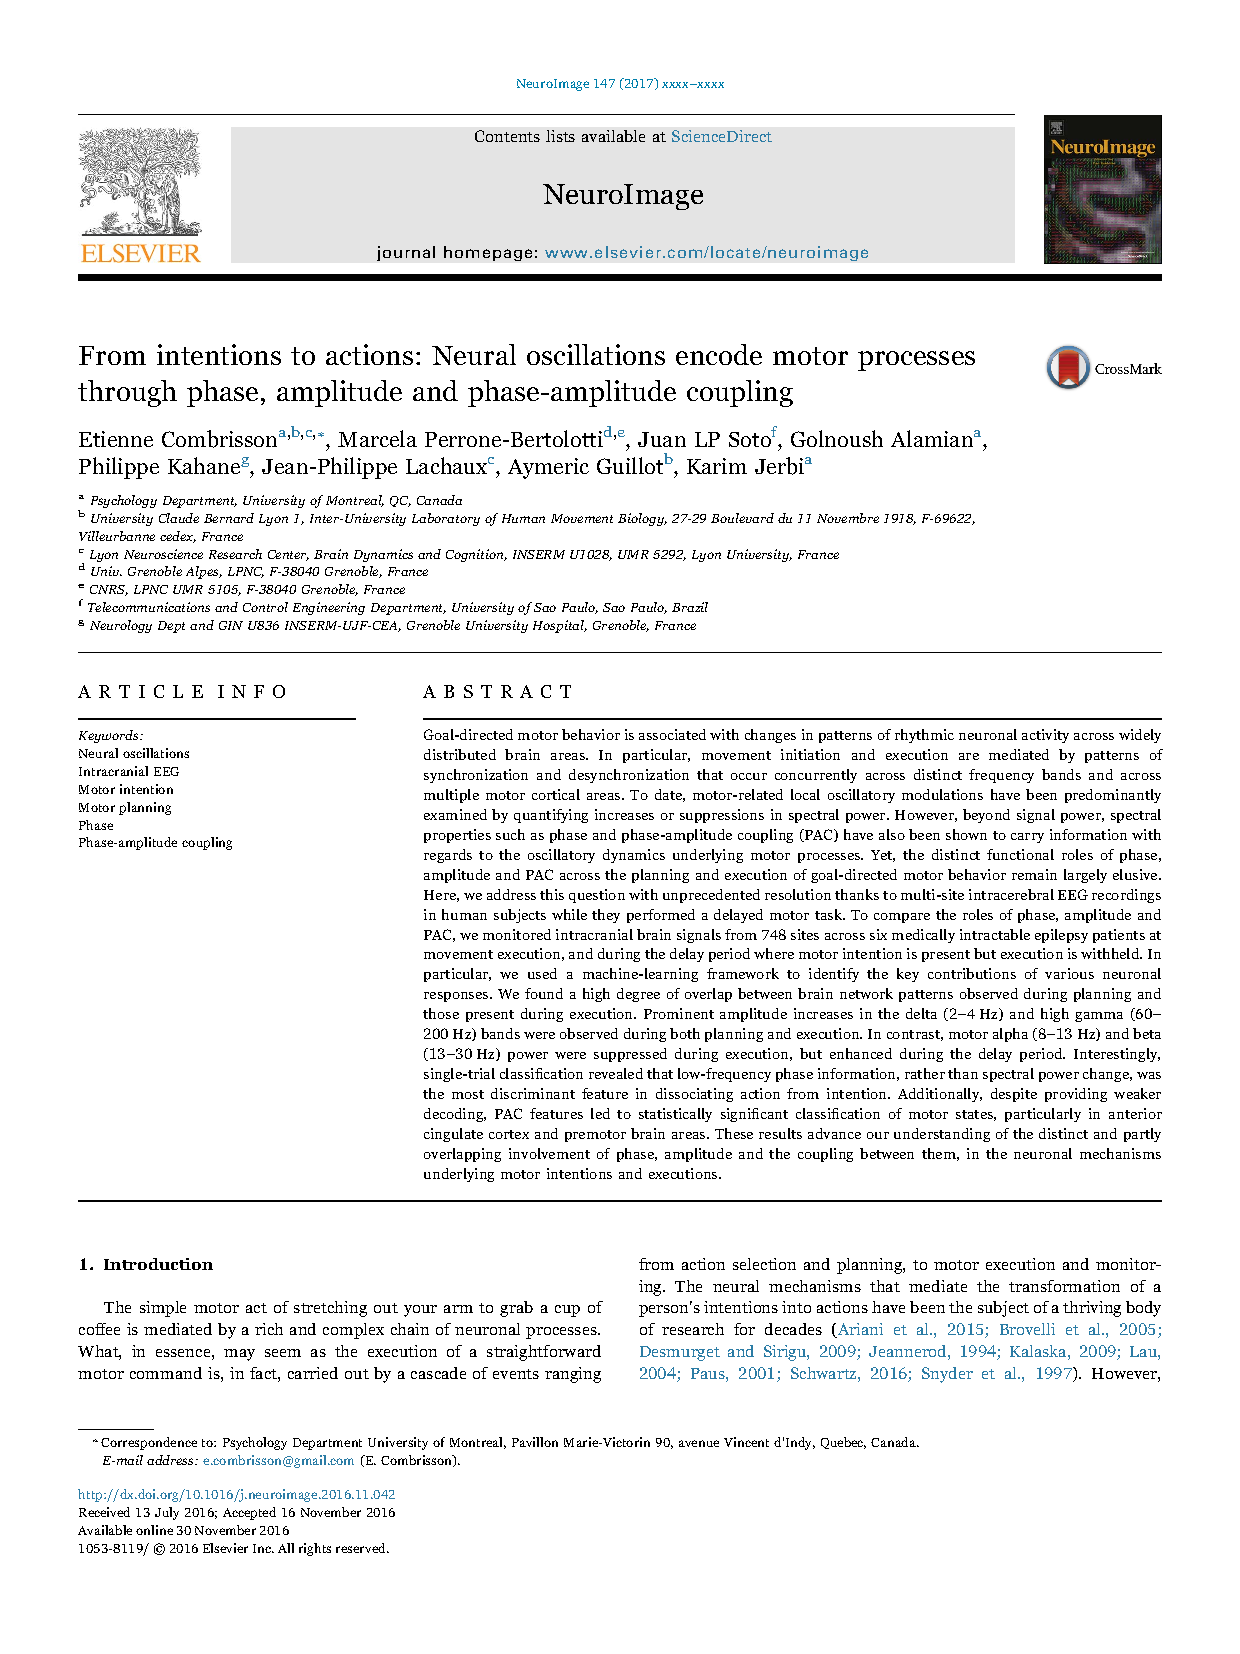
\includepdf[pages={1-29}]{Chap2/Etude2_Combrisson-etal-Encoding-Intention-Execution.pdf}


%%!TEX root = ../main.tex
\part{�tude 3: D�codage des directions de mouvement pendant et avant l'ex�cution de mouvement de membres sup�rieurs}
\label{Etude3_decodage}


\chapter*{Introduction}
Mon introduction


%%% --------------------------
%%% Article
%%% --------------------------
\includepdf[pages={1-28}]{Chap3/Combrisson-etal_Decoding-Intention-Execution.pdf}


%%!TEX root = ../main.tex
\part{�tude 4 : Tensorpac, logiciel Python de calcul de Phase-Amplitude Coupling}
\label{Etude4_tensorpac}
\pagestyle{headings}


\chapter*{Introduction}
Le \pacFR (PAC) est un marqueur qui mesure le degr�s de couplage entre la phase d'ondes lentes et l'amplitude d'ondes rapides. L'�valuation d'un couplage se fait de mani�re suivante :
\begin{itemize}    
    \item Extraction de la phase et de l'amplitude en utilisant soit des outils de filtrage suivi de la transform�e d'Hilbert, soit une transformation continue en ondelettes.
    \item Calcul du couplage entre ces deux signaux en utilisant une des m�thodologies existantes \citep{tort_measuring_2010,ozkurt_statistically_2012,canolty_high_2006}...
    \item Le PAC �tant une mesure sensible aux bruits, on construit une distribution de mesure de PAC pouvant arriver par chance.
    \item La v�ritable mesure de PAC est ensuite normalis�e par cette distribution de chance afin de minimiser le bruit.
\end{itemize}
Un nombre cons�quent de m�thodes ont �t� propos�es pour chacune de ces �tapes ce qui complique la comparaison et la reproductibilit�. De plus, toutes les publications introduisant de nouvelles m�thodes les pr�sentent en utilisant des vecteurs et ne fournissent pas l'adaptation matricielle ce qui ne prend pas en compte le format des donn�es (nombre de sujets, d'�lectrodes, d'essais...) et donc n'est pas du tout optimal d'un point de vue temps de calcul.\\
Dans ce contexte, nous avons mis en place une toolbox Python, \textit{Tensorpac}, d�di�e exclusivement au calcul du \pacFR. Dans cette toolbox les m�thodes sont impl�ment�es de fa�on modulaire ce qui signifie que l'utilisateur peut combiner les m�thodes existantes pour chacune des �tapes du calcul du PAC. D'autre part, \textit{Tensorpac} utilise des tenseurs permettant de g�n�raliser le calcul � partir de s�ries temporelles vers des donn�es multi-dimensionnelles. Cette impl�mentation en tenseurs est combin�e � du calcul en parall�le ce qui diminue encore le temps d'ex�cution et facilite l'envoie sur des serveurs de calcul. Ce paquet inclue �galement le calcul de comodulograme (soit en cherchant les couples (phase, amplitude) soit en fixant l'un des deux et en faisant varier la largeur de bande de l'autre), statistiques et la visualisation. Pour finir, \textit{Tensorpac} est distribu� sous une licence BSD et peut �tre t�l�charger sur Github \footnotemark[1] et nous fournissons �galement une documentation d�taill�e \footnotemark[2].

\footnotetext[1]{\url{https://github.com/EtienneCmb/tensorpac}}
\footnotetext[2]{\url{https://etiennecmb.github.io/tensorpac/}}


%%% --------------------------
%%% Article
%%% --------------------------
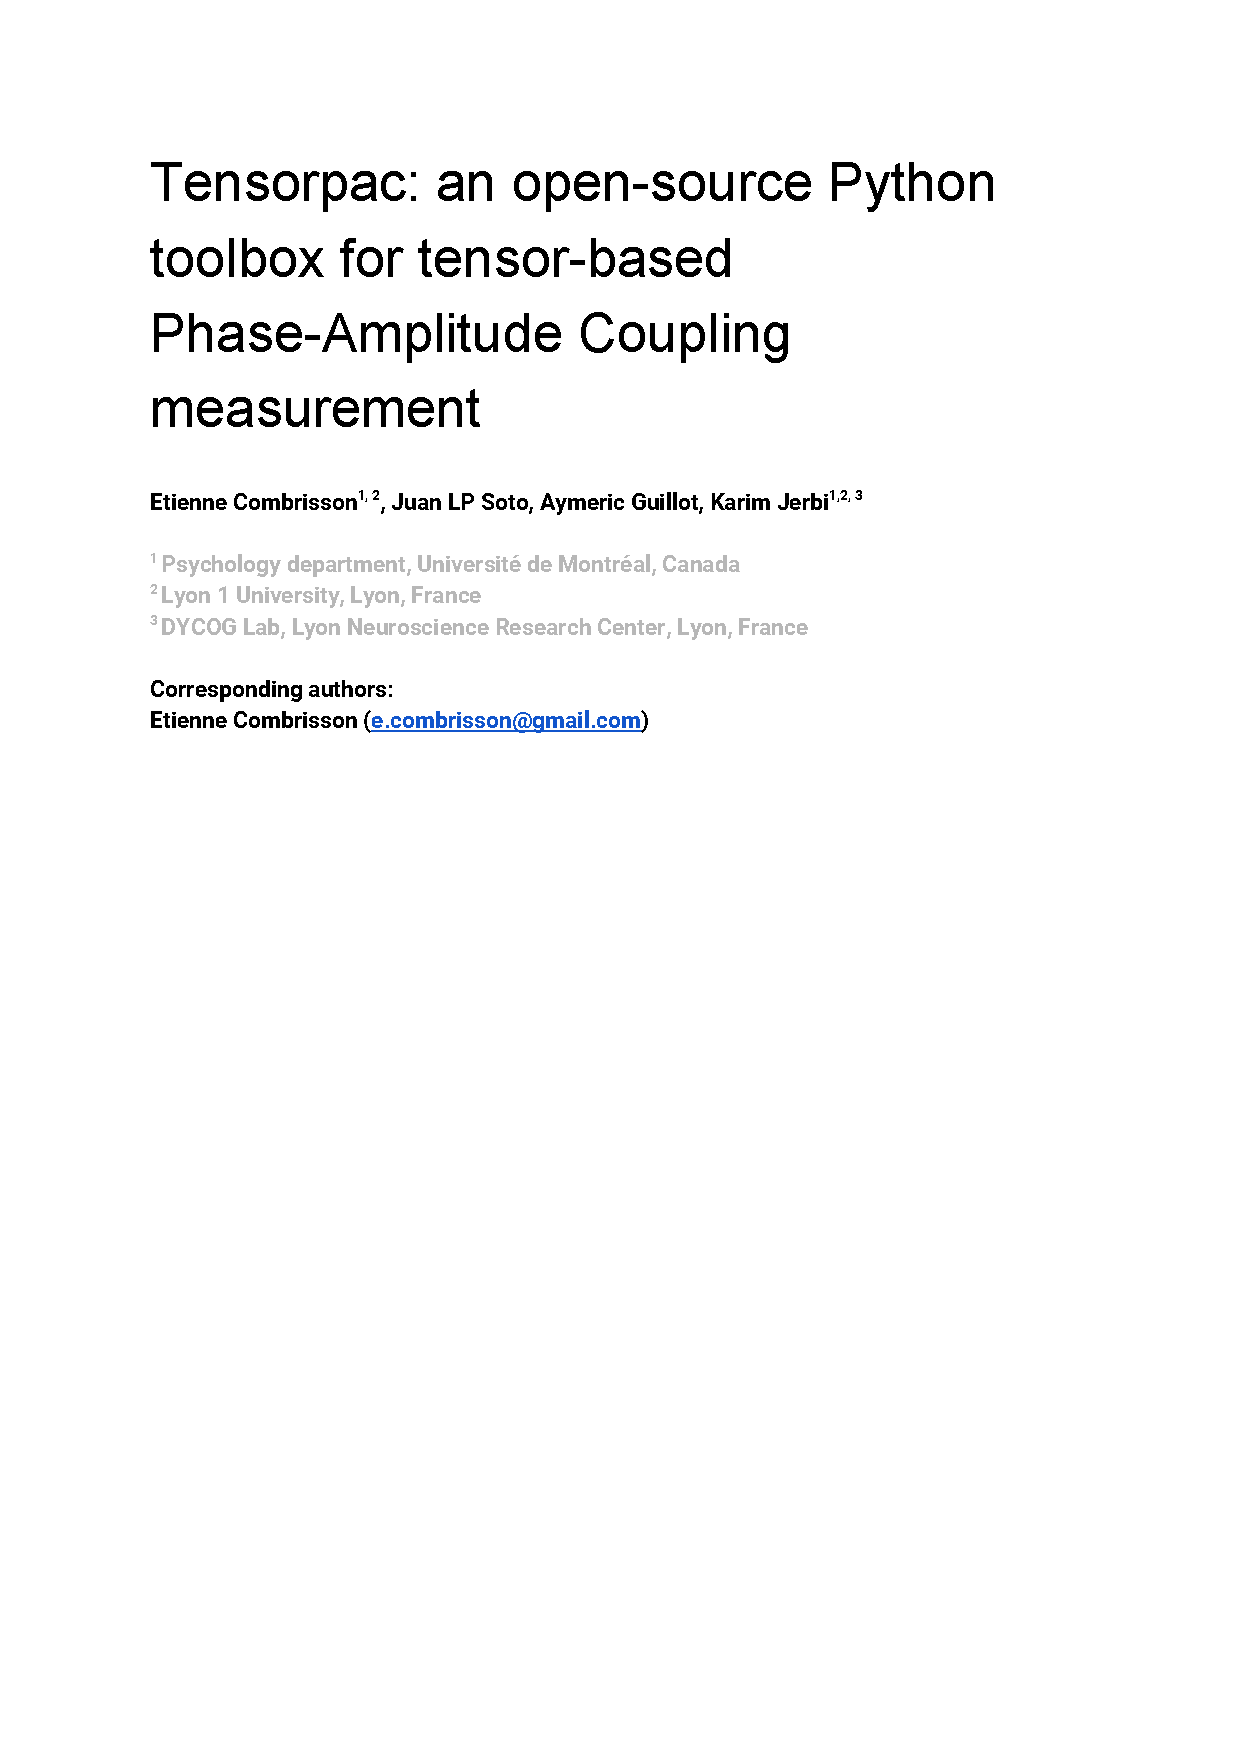
\includepdf[pages={1-18}]{Chap4/combrisson_2017_tensorpac.pdf}
%\part{�tude 5: d�codage des �motions}
\label{Etude5_emotions}


\chapter*{Introduction}
blabla Intro

\vspace{1\baselineskip}
Blabla �tude


%%% --------------------------
%%% Article
%%% --------------------------
%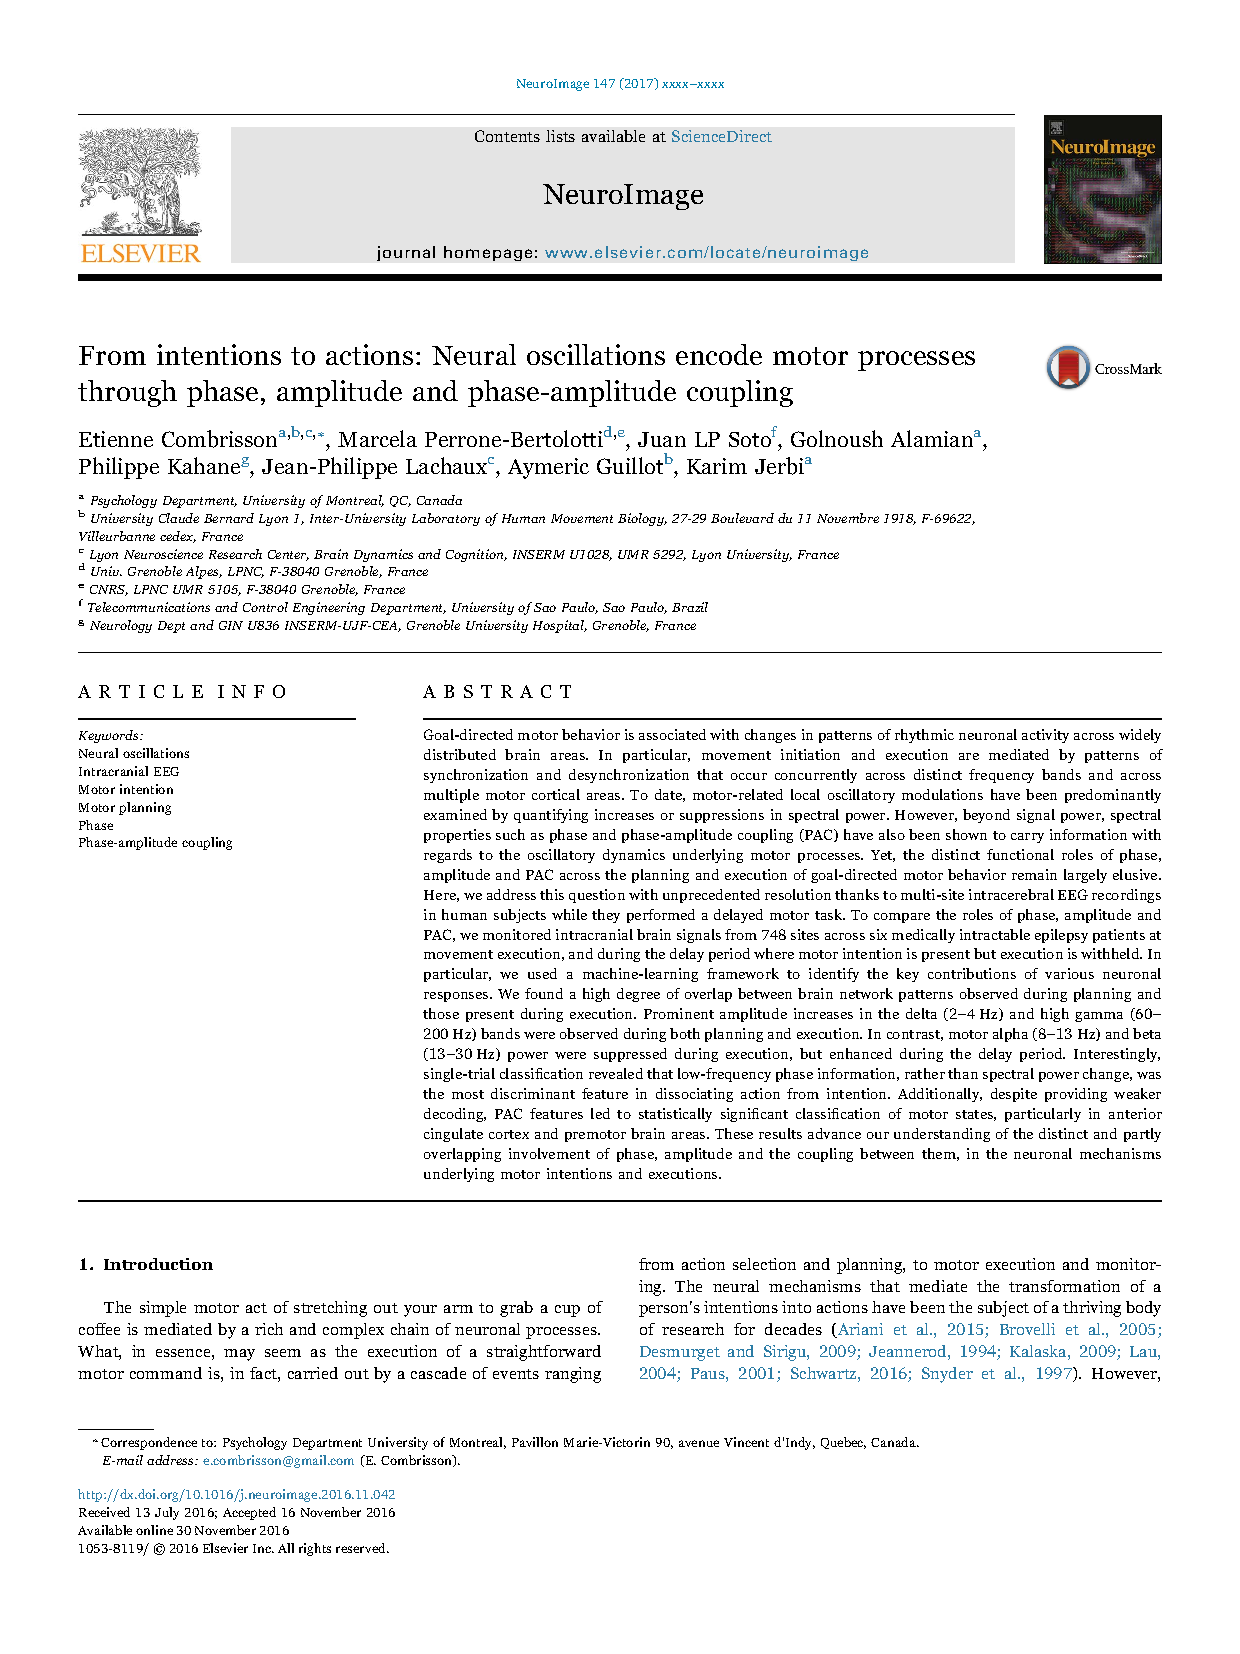
\includepdf[pages={1-29}]{Chap2/Etude2_Combrisson-etal-Encoding-Intention-Execution.pdf}




% ==================================================================
% CONCLUSION
\makeatletter
\renewcommand*{\toclevel@chapter}{-1}
\part{Discussion, conclusion et perspectives}
% \addcontentsline{toc}{chapter}{Conclusion g�n�rale}
\pagestyle{headings}

\chapter*{Discussion}

% Paragraphe 1-Vue d'ensemble de ce travail de th�se: Il s'est d�clin� en deux composante: Une contribution empirique [articles 2 et 3] et des contributions m�thodologiques (� la fois th�oriques [article 1] mais aussi en temre de d�veloppement logiciel [articles 4-6].

Ce travail de th�se s'articule autour de deux grands axes, (\textit{1}) un apport empirique permettant d'am�liorer notre compr�hension du r�le des composantes d'amplitude, de phase et de couplage phase-amplitude lors d'une t�che motrice dirig�e (articles 2 et 3). Nous avons utilis� des algorithmes de classification pour identifier les marqueurs les plus pertinents, (\textit{2}) un apport m�thodologique que ce soit d'un point de vue th�orique pour mieux comprendre la notion de seuil de chance en \textit{machine-learning} (article 1) et pratique via l'impl�mentation de plusieurs logiciels d'analyse et de visualisation (articles 4-6). \\

% Paragraphe 2-R�sum� des r�sultats les plus saillants obtenus dans les �tudes empiriques (articles 2 et 3)

Les deux articles empiriques partagent une m�me m�thodologie : l'utilisation des algorithmes de \textit{machine-learning} pour identifier les marqueurs de puissance, de phase et de PAC susceptibles de d�coder les �tats moteurs (article 2 cf. \ref{Etude2_encodage}) ou les directions motrices (article 3 cf. \ref{Etude3_decodage}). Cette premi�re �tude a permis de mettre en �vidence une augmentation significative de couplage $\alpha/\gamma$ durant la phase de repos qui s'att�nue ensuite durant l'ex�cution. D'un point de vue d�codage, la composante de phase tr�s basse fr�quence (\textit{VLFC}, $<1.5hz$) est le marqueur ayant montr� les plus forts taux de d�codage � travers toutes les conditions classifi�es (\textit{Repos Vs Pr�p.}, \textit{Repos Vs Exec.}, \textit{Pr�p. Vs Exec.}, \textit{Repos Vs Pr�p. Vs Exec.}). Dans une moindre mesure, le PAC pr�sente lui aussi des d�codages significatifs pour diff�rencier ces �tats moteurs ce qui n'est pas le cas pour diff�rencier les directions (article 3 cf \ref{Etude3_decodage}). En effet, le d�codage \textit{Up Vs Down Vs Left Vs Right} est majoritairement possible via des marqueurs de puissance. Durant l'ex�cution, la puissance des oscillations $\gamma$ permet de clairement diff�rencier les modulations � travers les directions dans les r�gions motrices et pr�-motrices. Plus important encore, le m�me ph�nom�ne a lieu lorsque la puissance dans la bande $\alpha$ dans le cortex pr�-moteur et frontal est utilis�e. Pris ind�pendamment, ces deux marqueurs en utilisation unique permettent d'obtenir des d�codages significatifs ($~70\%$ pour l'ex�cution et $~50\%$ durant la pr�paration). Pour finir, nous avons combin� plusieurs algorithmes de \textit{feature selection} ce qui a permis d'atteindre des d�codages proches de $90\%$ pour diff�rencier les quatre directions � la fois durant l'ex�cution et la pr�paration motrice. \\

% Paragraphe 3-Mettre en valeur la nouveaut�/originalit� de ces r�sultats (� quel point c'est diff�rent de ce qu'avait fait les autres chercheurs jusqu'ici?)

PARAGRAPHE DE CE QUI EST VRAIMENT NOUVEAU. \\

% Paragrpahe 4-Regard critique sur les 2 �tudes en intra: Les limitations de ces donn�es (nombre de patients, le fait qu'il s'agit de patient, le fait que les electrodes se trouvent � des endroits diff�rents � travers les patients, le fait que le d�lain'�tait pas variable, le fait qu'on avait pas acc�s syst�matique � l'onset du mouvement, etc etc).

Ces deux �tudes ont un certain nombre de limitations. Tout d'abord, les donn�es intracr�niennes �tant relativement rares, nous n'avons acc�s qu'aux donn�es de six sujets, chacun ayant approximativement une centaine d'�lectrodes. Au total, ces 6OO points d'enregistrement offrent une couverture partielle des r�gions c�r�brales. De plus, ces sujets souffrent d'une forme d'�pilepsie pharmacor�sistante ce qui limite la possibilit� de g�n�raliser � des sujets sains. L'implantation des sites intracr�niens �tant li�e � la localisation du foyer �pileptog�ne, il en r�sulte une implantation propre � chaque sujet et donc, d'une part il est tr�s difficile de pouvoir g�n�raliser le comportement d'un site en particulier puisqu'il est possible qu'il soit le seul dans cette r�gion et d'autre part, l'implantation n'�tant pas sym�trique elle ne permet pas d'�tudier l'effet controlat�ral et ipsilat�ral. La t�che utilis� pour mener � bien ces deux �tudes a �galement des limitations. Tout d'abord, tout les \textit{timing} sont fixes et donc, en l'absence de d�lais variables, il est tout � fait envisageable que les sujets puissent anticiper le d�but d'une phase au fur et � mesure que la t�che avance. De plus, le design de la t�che ne permet pas de conclure clairement sur le type de processus d�cod�s. En effet, on est en droit de se demander si l'on d�code une v�ritable pr�paration/ex�cution de mouvements ou un processus attentionnel, visuomoteur, s�lection spatiale ou d'imagerie motrice. Pour finir, apr�s l�apparition d'un signal visuel, les donn�es ne permettaient pas d'avoir acc�s au d�but du mouvement. Ainsi, l'activit� neuronale contenue dans les tanches temporelles qui suivent directement l'apparition du signal visuel peut contenir des �v�nements diff�rents d� � la variabilit� du temps de r�action d'un essais � l'autre. Les outils de \textit{machine-learning} �tant justement entra�n�s � travers les essais, l'alignement sur le \textit{go-signal} pourrait alors d�grader la performance de classification. \\

% Paragraphe 5-Pour quoi est-ce que malgr�s ces limitations nous avons confiance dans les r�sultats obtenus?

Pour pouvoir g�n�raliser les �tudes 2 et 3 aux sujets sains, les �lectrodes proches des yeux ou contenant une activit� �pileptiforme sont syst�matiquement rejet�es. De plus, les analyses sont appliqu�es � travers les essais ce qui permet de minimiser l'activit� c�r�brale qui n'est pas directement reli�e � la t�che. M�me si les six sujets offrent une couverture partielle, ils ont �t� s�lectionn�s pour leur implantation pr�-frontale, frontale et pari�tale \cad l� o� l'on attend les meilleurs r�sultats de d�codage d'une t�che motrice. L'�tude de la lat�ralit� est une limitation propre � tout les enregistrements invasifs et devrait donc �tre trait� avec des enregistrements d'EEG de scalp ou de MEG. L'impact du d�lai fixe et de l'alignement sur le \textit{go-signal} de la t�che ont �t� minimis�s de fa�on diff�rentes dans chacune de ces deux �tudes. Dans la premi�re (cf. \ref{Etude2_encodage}) la fen�tre de d�codage consid�r�e pour diff�rencier les �tats moteurs se situent 500ms apr�s le \textit{go-signal} et donc, devrait limiter l'utilisation d'une activit� neuronale non-pertinente. Dans le second article (cf. \ref{Etude3_decodage}, le d�codage des directions se fait dans un esprit \textit{temps-r�el}. Un classifieur est syst�matiquement r�-entra�n� puis test� dans les diff�rentes fen�tres temporelles d�finies (67 au total), du d�but du repos � la fin de l'ex�cution. En cons�quence, seule 2/67 fen�tres qui suivent les deux indications visuelles peuvent potentiellement montrer des d�codages plus bas. \\

% Paragraphe 6-R�sumer l'apport de d�veloppement logiciel (re-mentionner les packages, et le nombre de lignes de code par package). Indiquer qu'ils peuvent �tre utilis�s pour des applications diverses et vari�es au-del� de ce pourquoi ces outils ont �t� d�velopp�s au d�part (les donn�es motrices en intra etc.). Indiquer en quelques lignes des d�veloppments futurs pr�vus pour certains de ces outils et le d�sir d'encourager d'autres personnes � contribuer activement au d�veloppment de ces outils das un esprit de partage/communautaire etc  (ce ne sont que des id�es bien sur)

Pour finir, tout les r�sultats d'analyses et de visualisation de cette th�se sont issus des logiciels Python open-source d�velopp�s � cet effet. \textit{Brainpipe} ($7899$ lignes) permet d'extraire des marqueurs de l'activit� neuronale (tel que l'amplitude, puissance, phase \dots) et de les classifier en utilisant \textit{Scikit-Learn}. \textit{Tensorpac} ($2230$ lignes), autre paquet Python open-source, permet de calculer le \pacFR avec une impl�mentation modulaire des m�thodes le tout reposant sur des calculs bas�s sur des tenseurs et mise en parall�le. Pour finir \textit{Visbrain} ($30771$ lignes) permet d'obtenir de visualiser de nombreux types de donn�es (pour du \textit{data-mining}, avec cerveau MNI semi-transparent, donn�es de sommeil \dots). Ces trois principaux paquets ont d'abord �t� d�velopp�s pour couvrir nos besoins. Puis, dans un d�sir de partager nos outils, ils ont �t� enti�rement reformat�s pour �tre utilisable par d'autre. \textit{Brainpipe} �tant le premier paquet d�velopp�, pourrait �tre tr�s largement am�lior� (surtout dans la gestion des dimensions des donn�es et de la m�moire RAM). \textit{Tensorpac} et \textit{Visbrain} n'ont pas ce soucis puisqu'ils ont �t� entam�s apr�s une connaissance plus mature du langage Python. Toutefois, de nombreuses autres m�thodologies pourraient �tre ajout�es � \textit{Tensorpac}, certaines �tant plus dur que d'autres � �tre impl�ment�es en tenseurs. Pour finir, \textit{Visbrain} � une longue feuille de route de pr�vue pour son d�veloppement futur, incluant de nombreuses refontes, am�liorations et surtout l'ajout de nouveaux modules de visualisations. Quoi qu'il en soit, avec leur qualit�s et leurs d�fauts, ces trois logiciels viennent avec un code extr�mement comment�, des datasets et exemples et des documentations. Mon plus grand souhait �tant que d'autres personnes participent � faire avancer ces projets tout en conservant l'id�e principale, un partage libre pour une science ouverte. 

\chapter*{Conclusion et perspectives futurs}

[1/2 page suffira]

2 id�es � d�velopper

(i) Un truc du genre "Taken together, this body of research advances our understanding of the role of oscillatory power, phase and PAC in goal-directed behavior, and provides efficient open-source packages for the scientific community to replicate and extend this research."

(ii) Proposer des pistes prometteuses pour l'avenir: Par exemple le fait de s'orienter d�finitivement vers des �tudes du syst�me moteur dans de grandes cohortes de sujets (via le data sharing et �tude multi-centriques) et via le open-science et le partage des outils d'analyses pou rrenforcer la reproductiblit� des r�sultats etc.


% ==================================================================
% ANNEXES
\let\cleardoublepage\clearpage
{
\hypersetup{linkcolor=black}
\appendix
\renewcommand*{\toclevel@section}{0}
\pagestyle{plain}

% *****************************************************************
%                   BCI MAP
% *****************************************************************
\section{Cartes des Interfaces Cerveau-Machine \citep{graimann_braincomputer_2009}}
\begin{figure}[H]
	\centering
	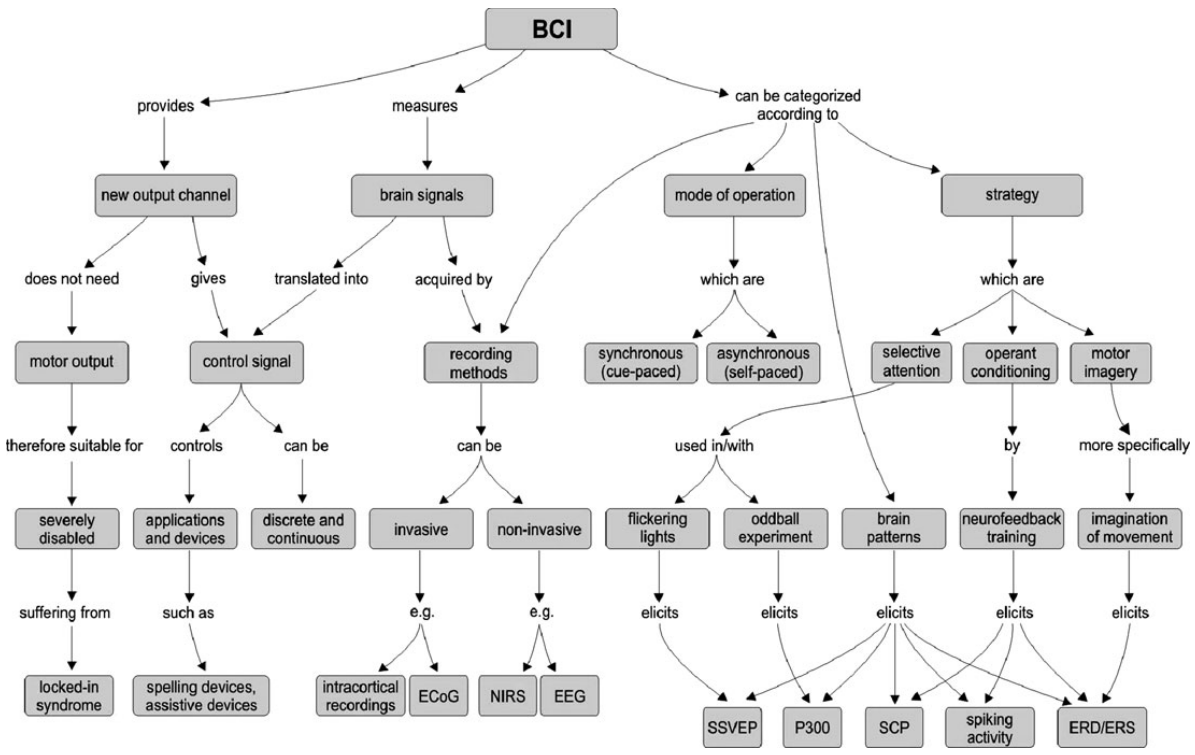
\includegraphics[scale=0.5,angle=-90]{./figures/Grainmann_2002_ICM_map}
	\caption{Cartes des Interfaces Cerveau-Machine \citep{graimann_braincomputer_2009}}
	\label{bci_map}
\end{figure}

% *****************************************************************
%                   BCI COMPETITION
% *****************************************************************
\section{Jeux de donn\'{e}es en libre acc\`{e}s (\textit{BCI competition})}
\begin{figure}[H]
	\begin{tabular}{|c|c|c|p{8cm}|}
		% COMPETITION II
		\hline
		\multicolumn{4}{|c|}{\href{http://www.bbci.de/competition/ii/}{BCI Competition II}} \tabularnewline
		\hline
		Set & N-Classes & Channel & Challenge \tabularnewline
		\hline
		Ia/Ib & 2 & 6-EEG & Decide whether the subject tried to produce cortical negativity or cortical positivity \tabularnewline
		\hline
		IIa & 4 & 64-EEG & Provide the intended target of the feedback test trials  \tabularnewline
		\hline
		IIb & 36 & 64-EEG & Estimate to which letter of a 6-by-6 matrix with successively intensified rows resp. columns the subject was paying attention to  \tabularnewline
		\hline
		III & 2 & 3-EEG & Provide a continuous output that could be used for a BCI- feedback \tabularnewline
		\hline
		IV & 2 & 28-EEG & Predict the laterality of upcoming finger movements (left vs. right hand) 130 ms before keypress \tabularnewline
		\hline

		% COMPETITION III
		\multicolumn{4}{|c|}{\href{http://www.bbci.de/competition/iii/}{BCI Competition III}} \tabularnewline
		\hline
		I & 2 & 64-ECoG & Cued motor imagery (left pinky, tongue) from one subject \tabularnewline
		\hline
		II & 36 & 64-EEG & Estimate to which letter of a 6-by-6 matrix with successively intensified rows resp. columns the subject was paying attention to \tabularnewline
		\hline
		IIIa & 4 & 60-EEG & Cued motor imagery with 4 classes (left hand, right hand, foot, tongue) from 3 subjects. Measure: kappa-coefficient \tabularnewline
		\hline
		IIIb & 2 & 2-EEG & Cued motor imagery with online feedback with 2 classes (left hand, right hand). Measure: mutual information \tabularnewline
		\hline
		IVa/IVb/IVc & 2 & 118-EEG & Cued motor imagery with 2 classes (right hand, foot) from 5 subjects \tabularnewline
		\hline
		V & 3 & 32-EEG & Cued mental imagery with 3 classes (left hand, right hand, word association) from 3 subjects \tabularnewline
		\hline
	
		% COMPETITION IV
		\multicolumn{4}{|c|}{\href{http://www.bbci.de/competition/iv/}{BCI Competition IV}} \tabularnewline
		\hline
		I & 2 & 64-EEG & Motor imagery (2 classes of left hand, right hand, foot) \tabularnewline
		\hline
		IIa & 4 & 22-EEG & Cued motor imagery (left hand, right hand, feet, tongue)   \tabularnewline
		\hline
		IIb & 2 & 3-EEG & Cued motor imagery (left hand, right hand)   \tabularnewline
		\hline
		III & 4 & 10-MEG & Decoding directions of finger/hand/wrist movements \tabularnewline
		\hline
		IV & 5 & 64-ECoG & Discrimination of movements of individual fingers \tabularnewline
		\hline
	\end{tabular}
	\caption{Jeux de donn\'{e}es en libre acc\`{e}s (\textit{BCI competition})}
	\label{annexe_bci_competition}
\end{figure}

% *****************************************************************
%                   COMPARATIF PAC
% *****************************************************************
\section{Comparatif de m\'{e}thodes PAC \citep{tort_measuring_2010}}
\begin{figure}[H]
	\centering
	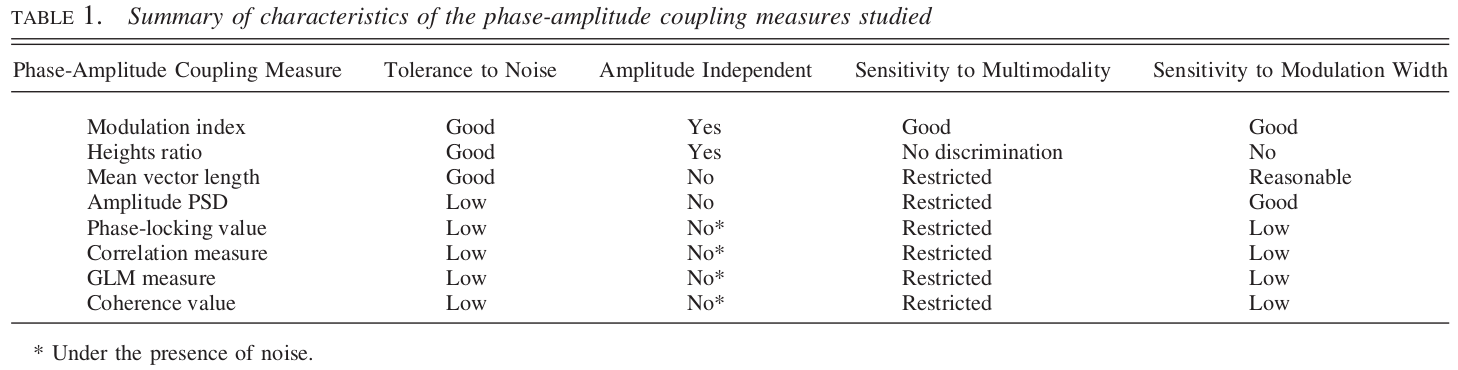
\includegraphics[scale=0.4,angle=-90]{./figures/PAC_methods_comparison}
	\caption{Comparatif de m\'{e}thodes PAC \citep{tort_measuring_2010}}
	\label{comp_pac}
\end{figure}

% *****************************************************************
%                   CLASSIFICATION PIPELINE
% *****************************************************************
\section{Pipeline standard de classification}
\begin{figure}[H]
	\centering
	\makebox[\textwidth][c]{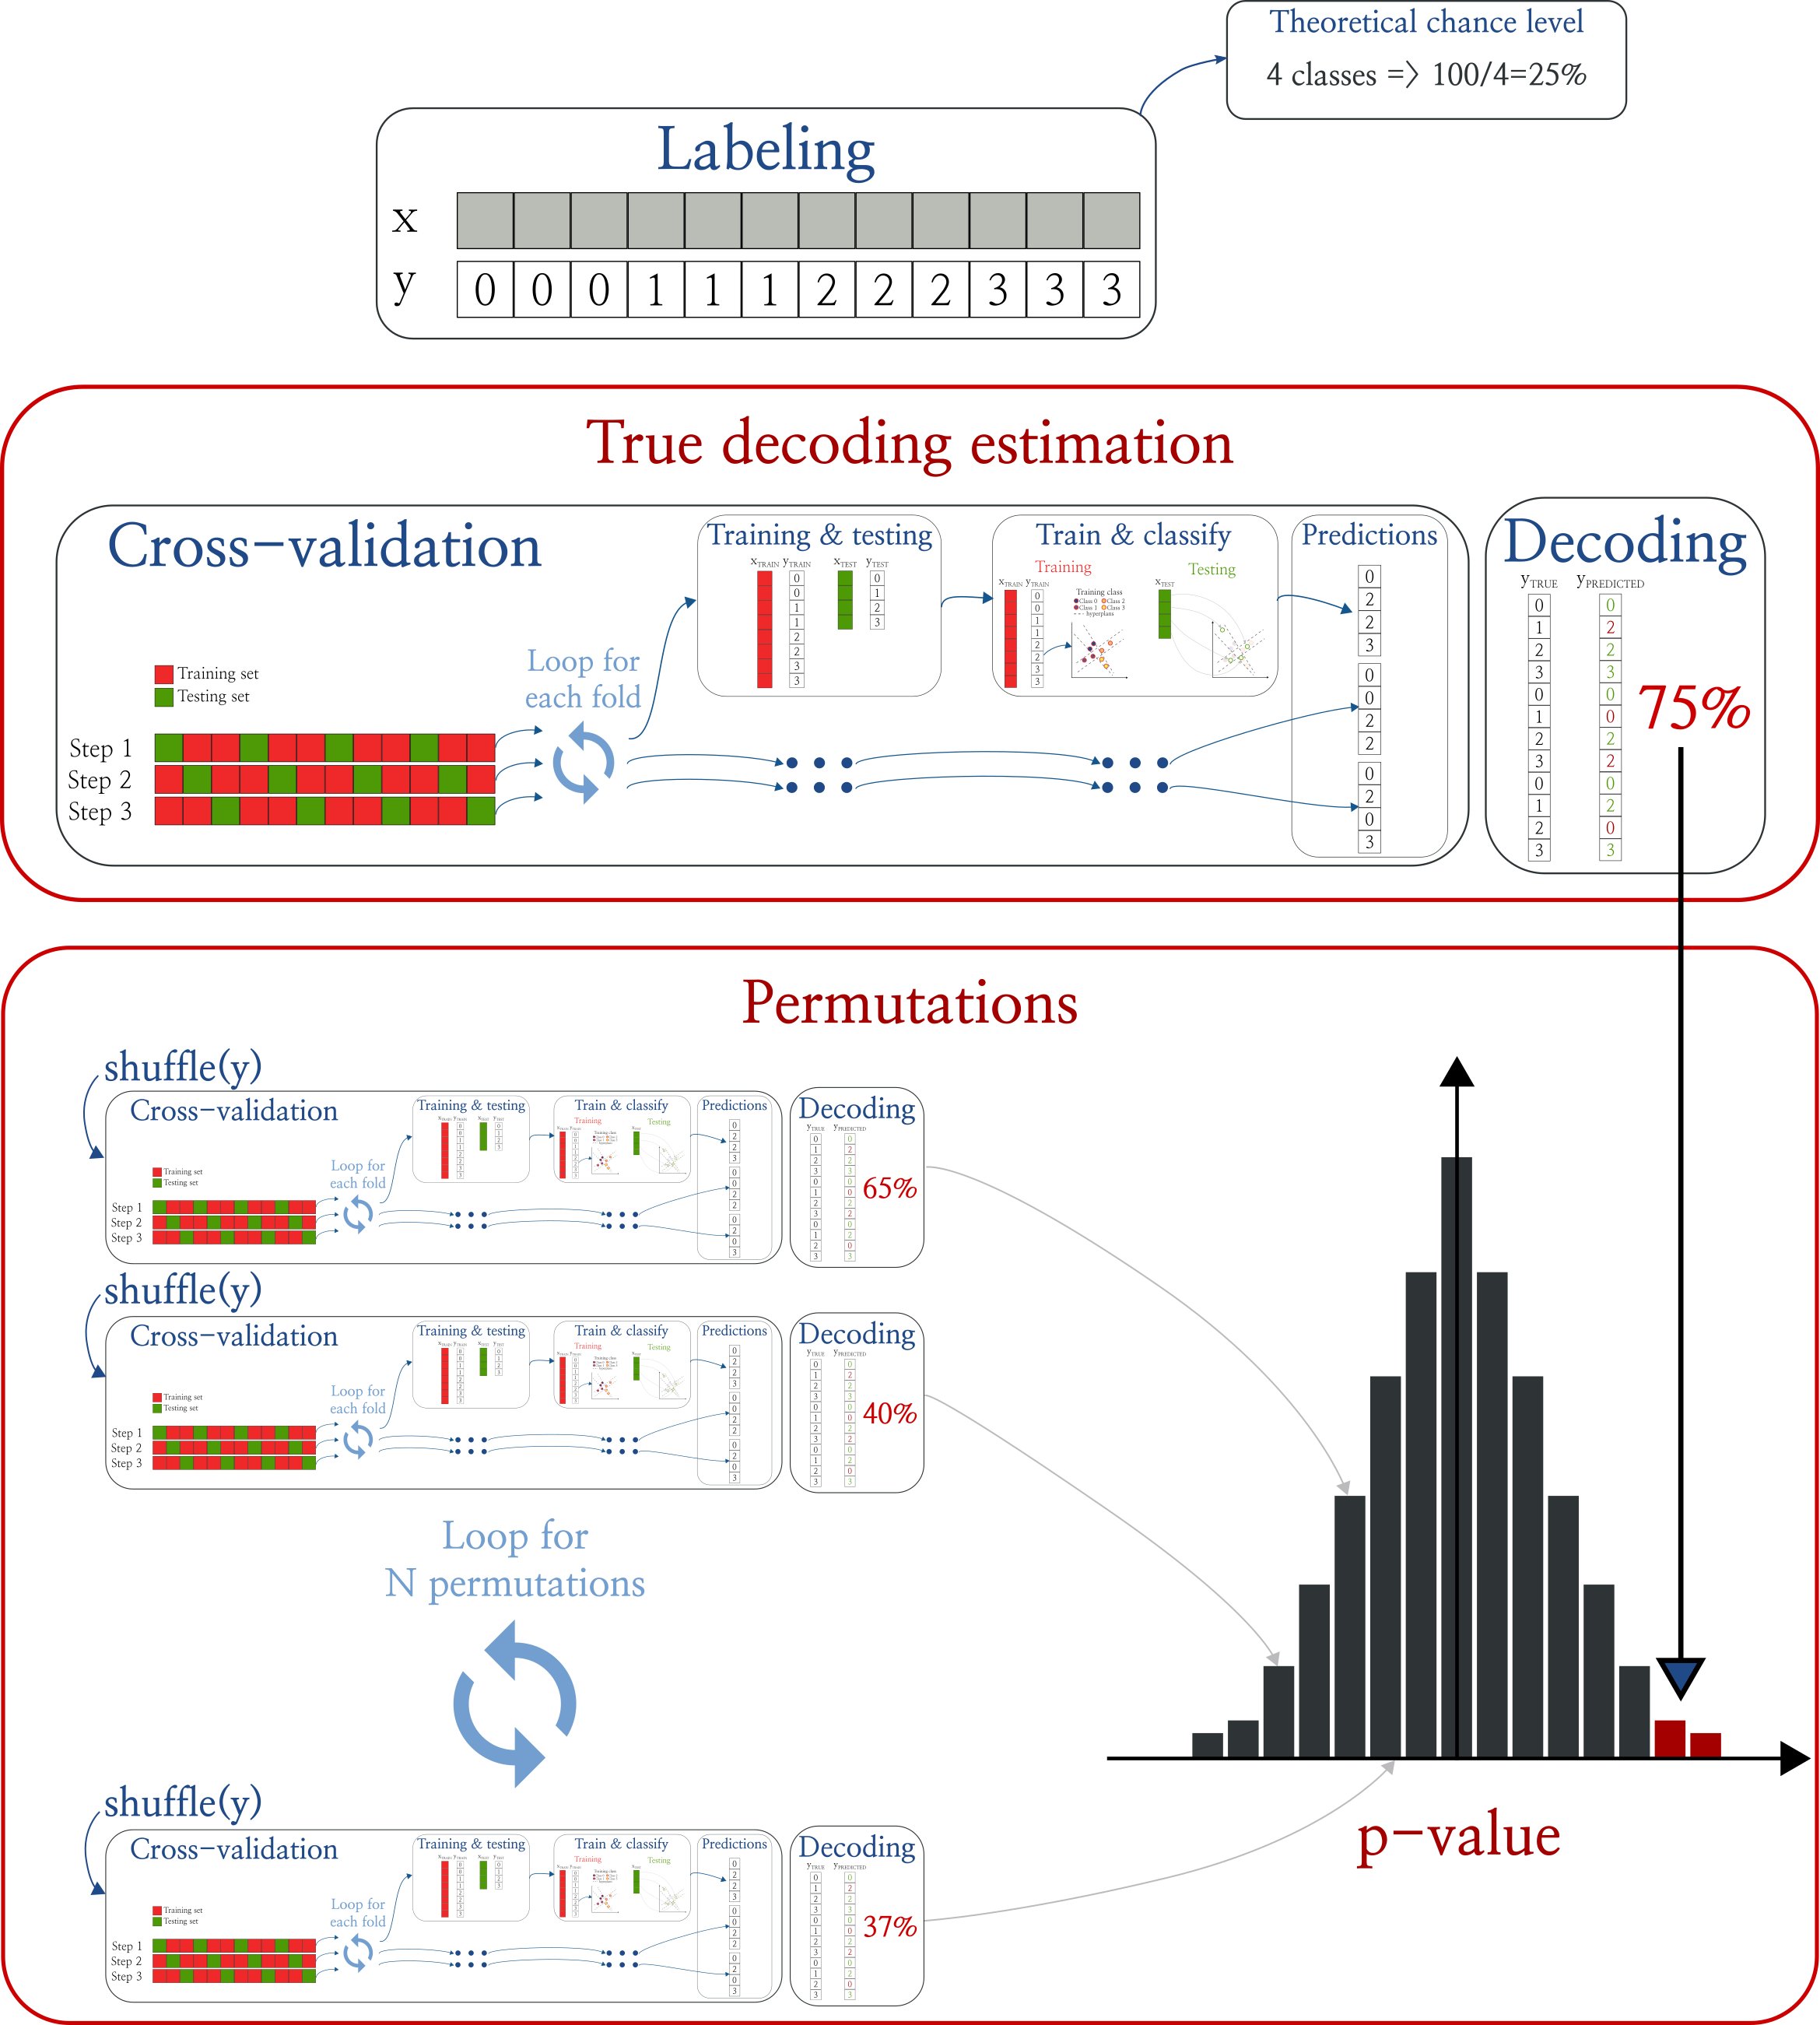
\includegraphics[scale=0.9]{./figures/clf_pipeline}}
	\caption{Pipeline standard de classification}
	\label{clf_pip}
\end{figure}

% *****************************************************************
%                   COMPARATIF CLASSIFIEURS
% *****************************************************************
\section{Comparatif de classifieurs \citep{scikit-learn}}
\begin{figure}[H]
	\centering
	\makebox[\textwidth][c]{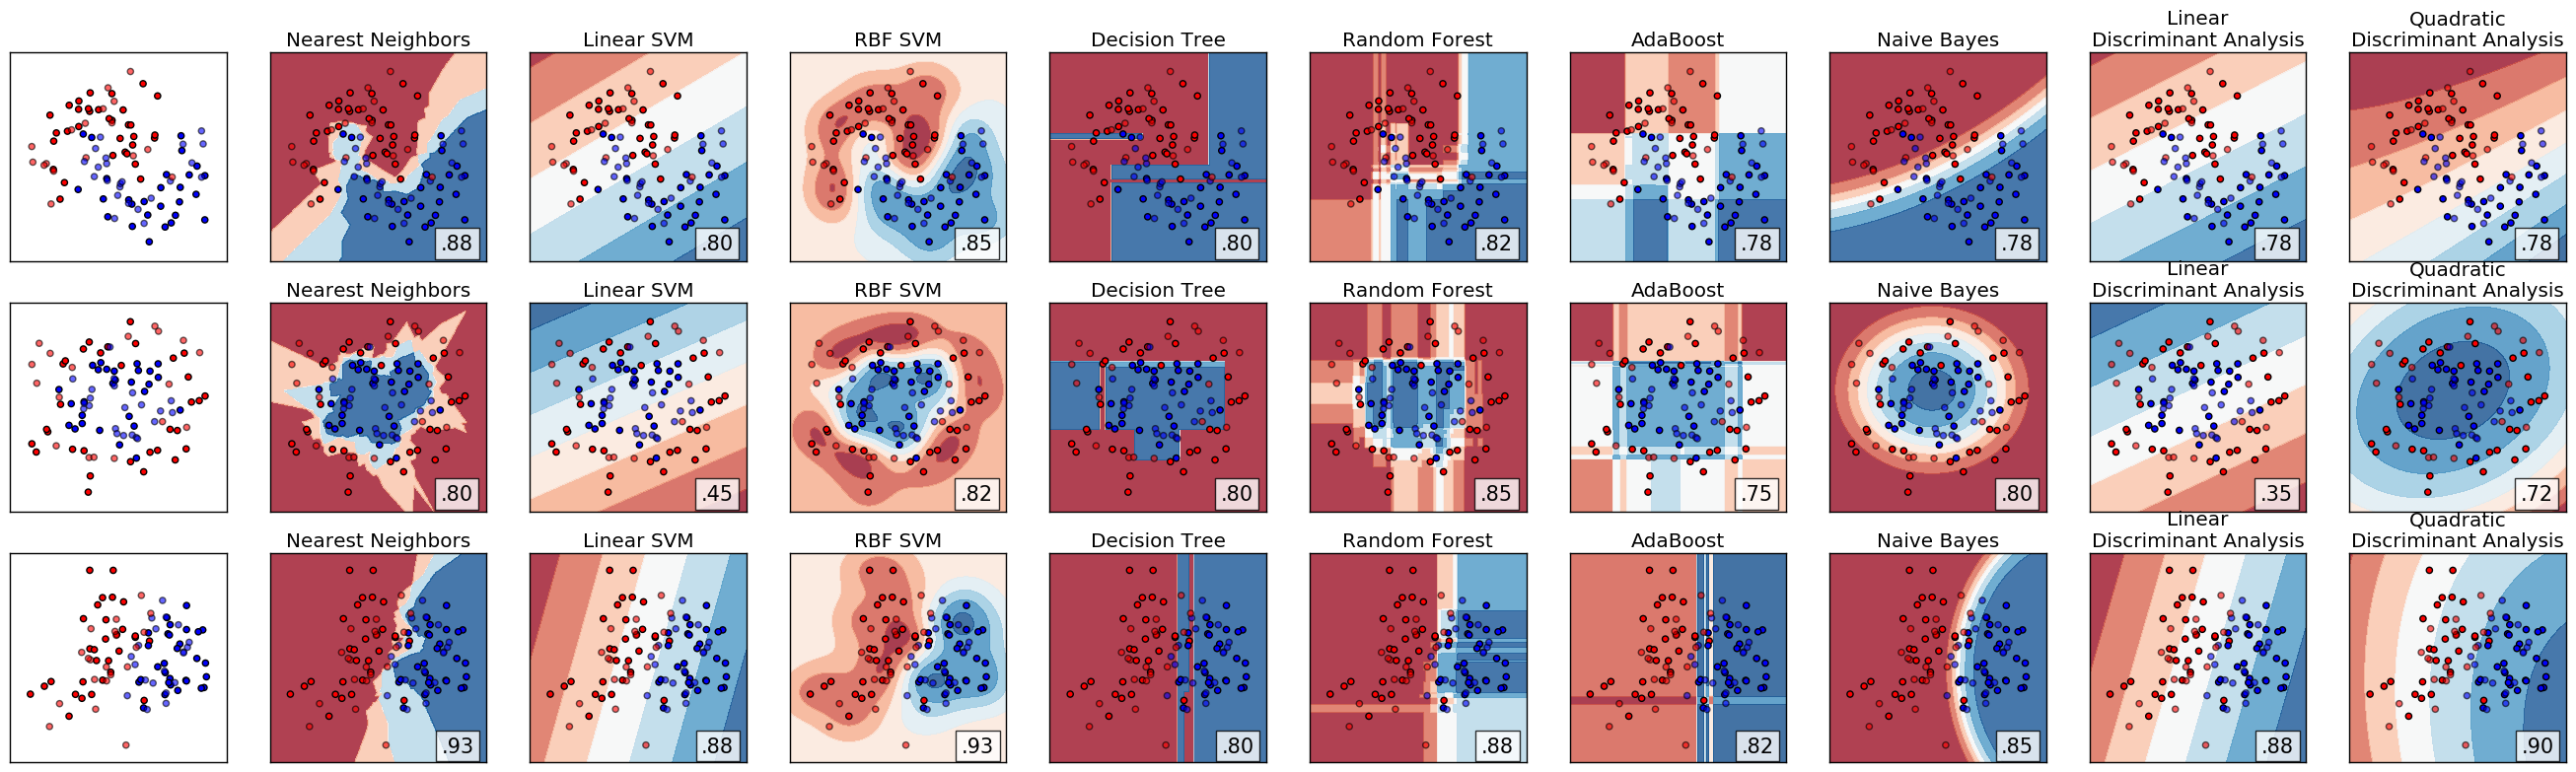
\includegraphics[scale=0.35,angle=-90]{./figures/classifier_comp}}
	\caption{Comparatif de classifieurs \citep{scikit-learn}}
	\label{comp_clf}
\end{figure}


% *****************************************************************
%                   SCHEMA IMPLANTATION
% *****************************************************************
\section{Exemple de sch\'{e}ma d'implantation}
\begin{figure}[H]
	\centering
	\makebox[\textwidth][c]{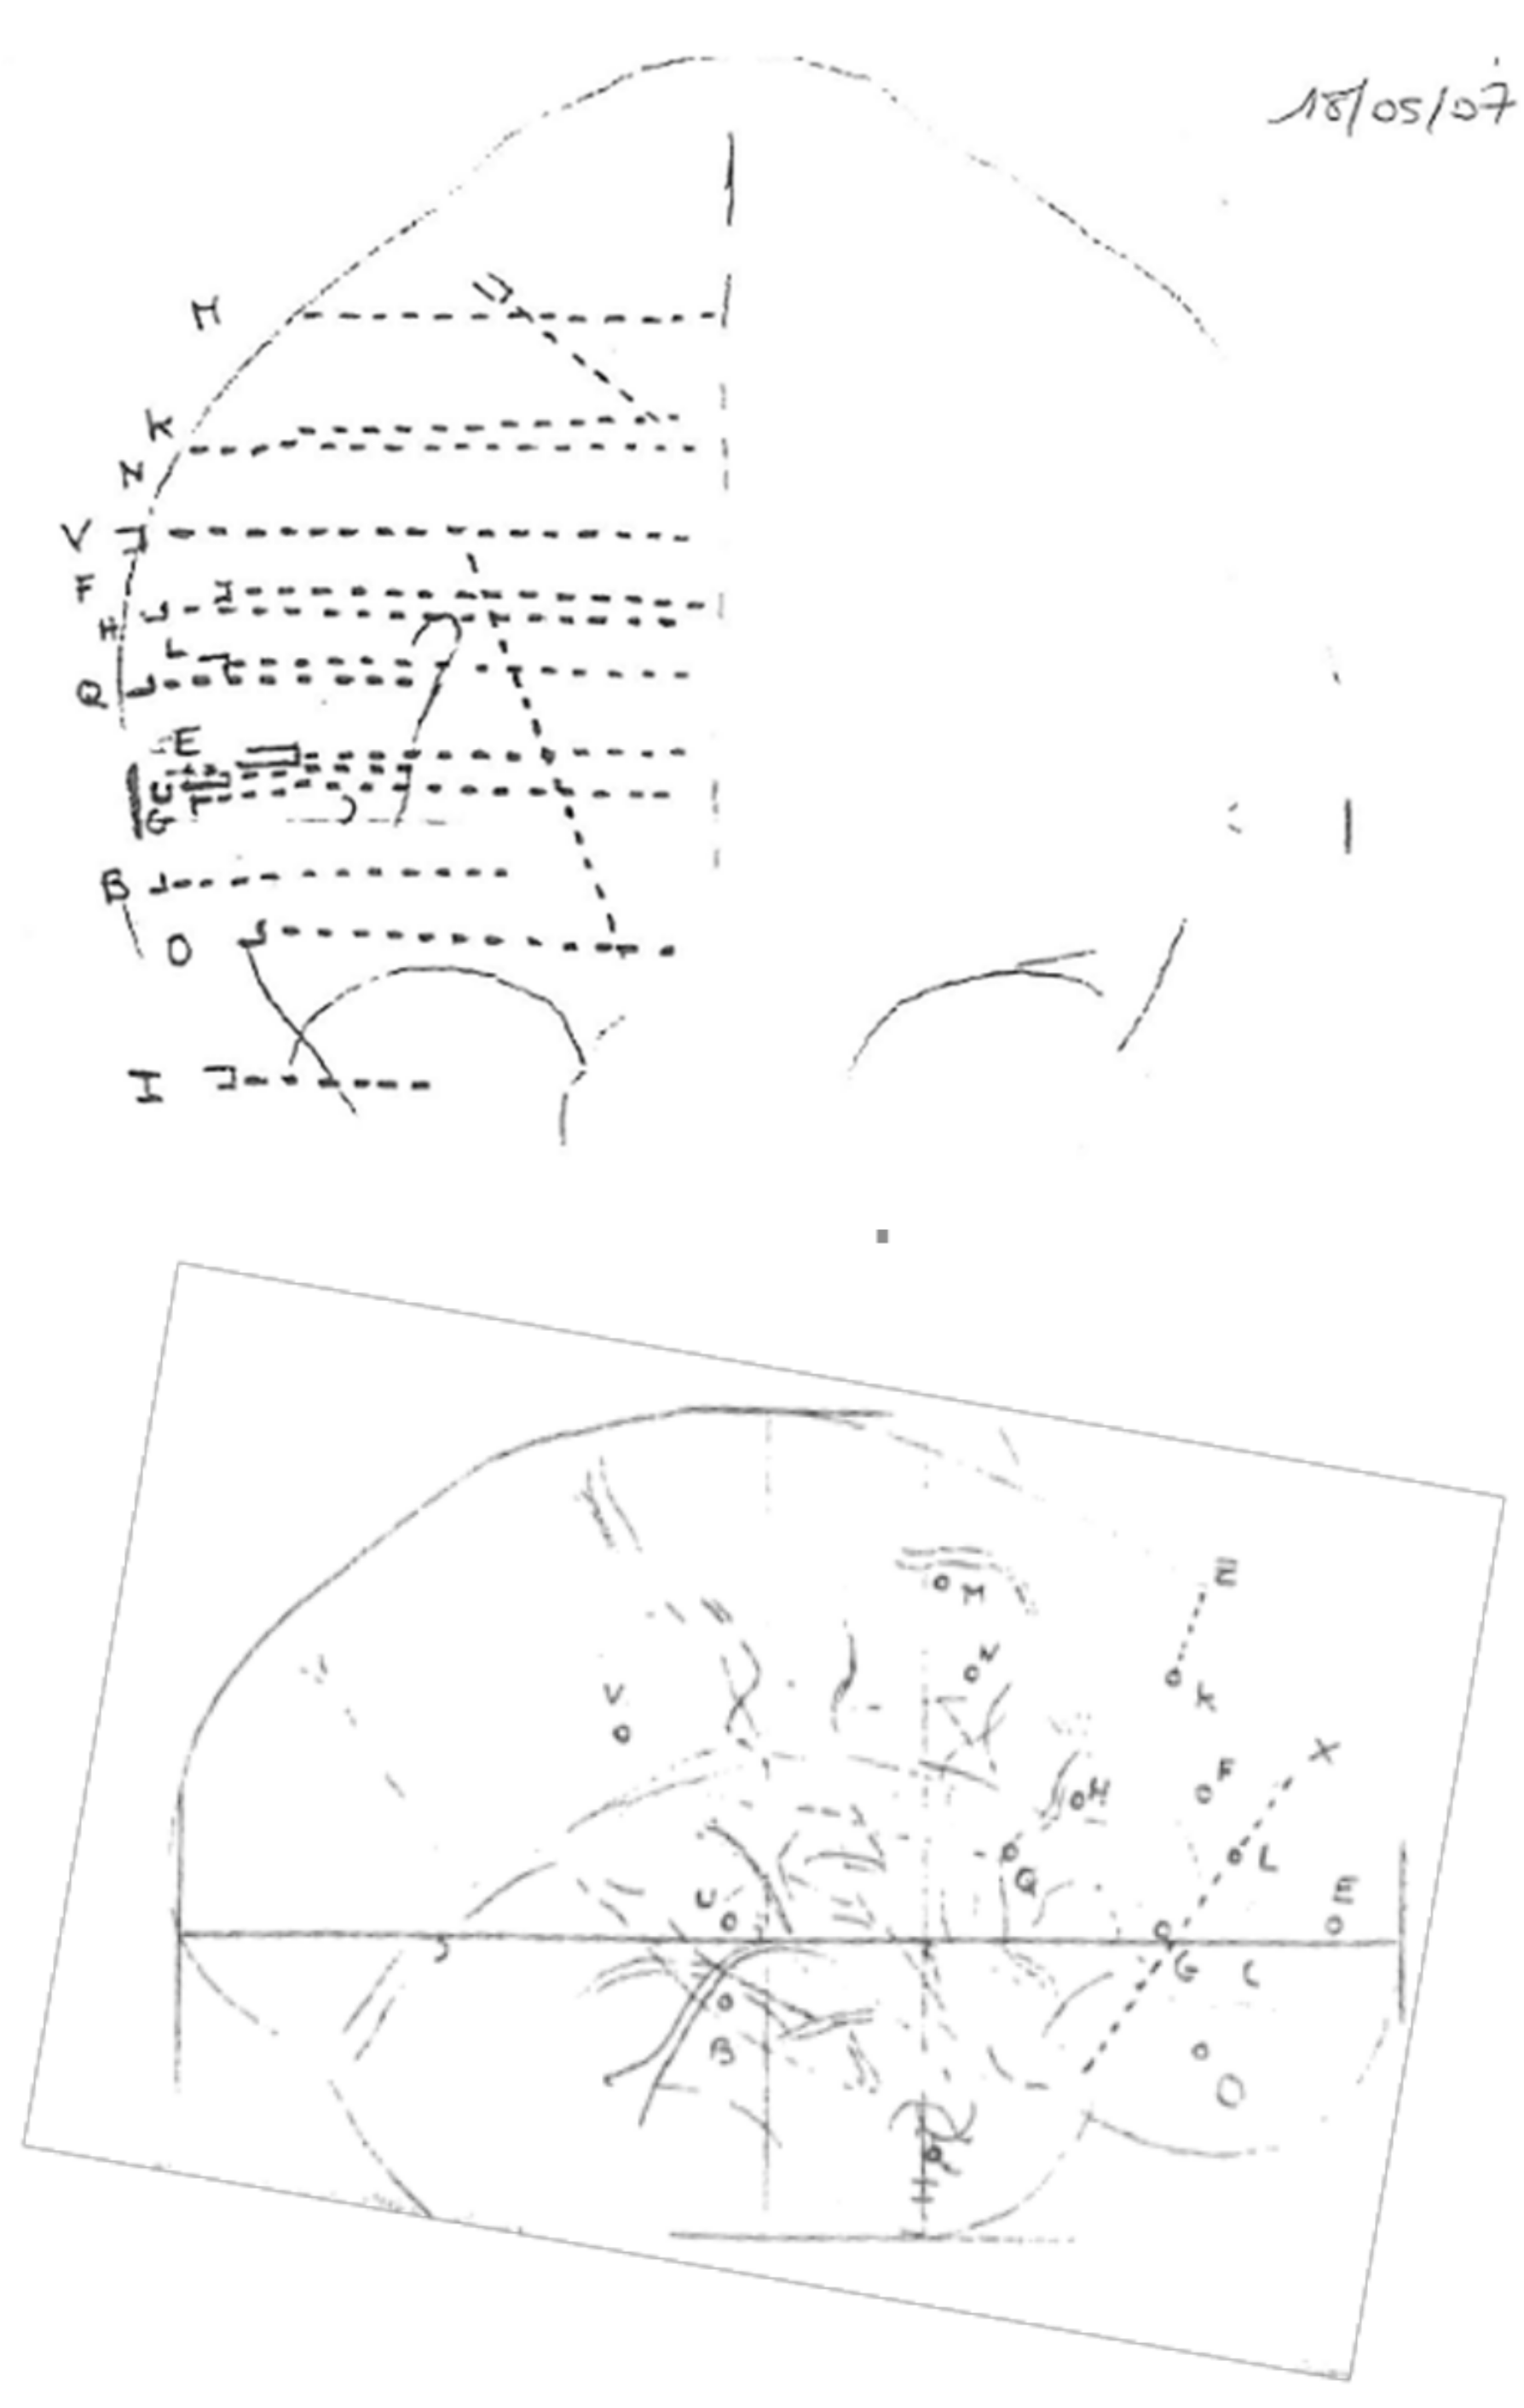
\includegraphics[scale=1]{./figures/schema-implantation_annexe}}
	\caption{Exemple de sch\'{e}ma d'implantation}
	\label{schema_implantation}
\end{figure}

% *****************************************************************
%                   DOCUMENTATION DE BRAINPIPE
% *****************************************************************
\section{Documentation de brainpipe}
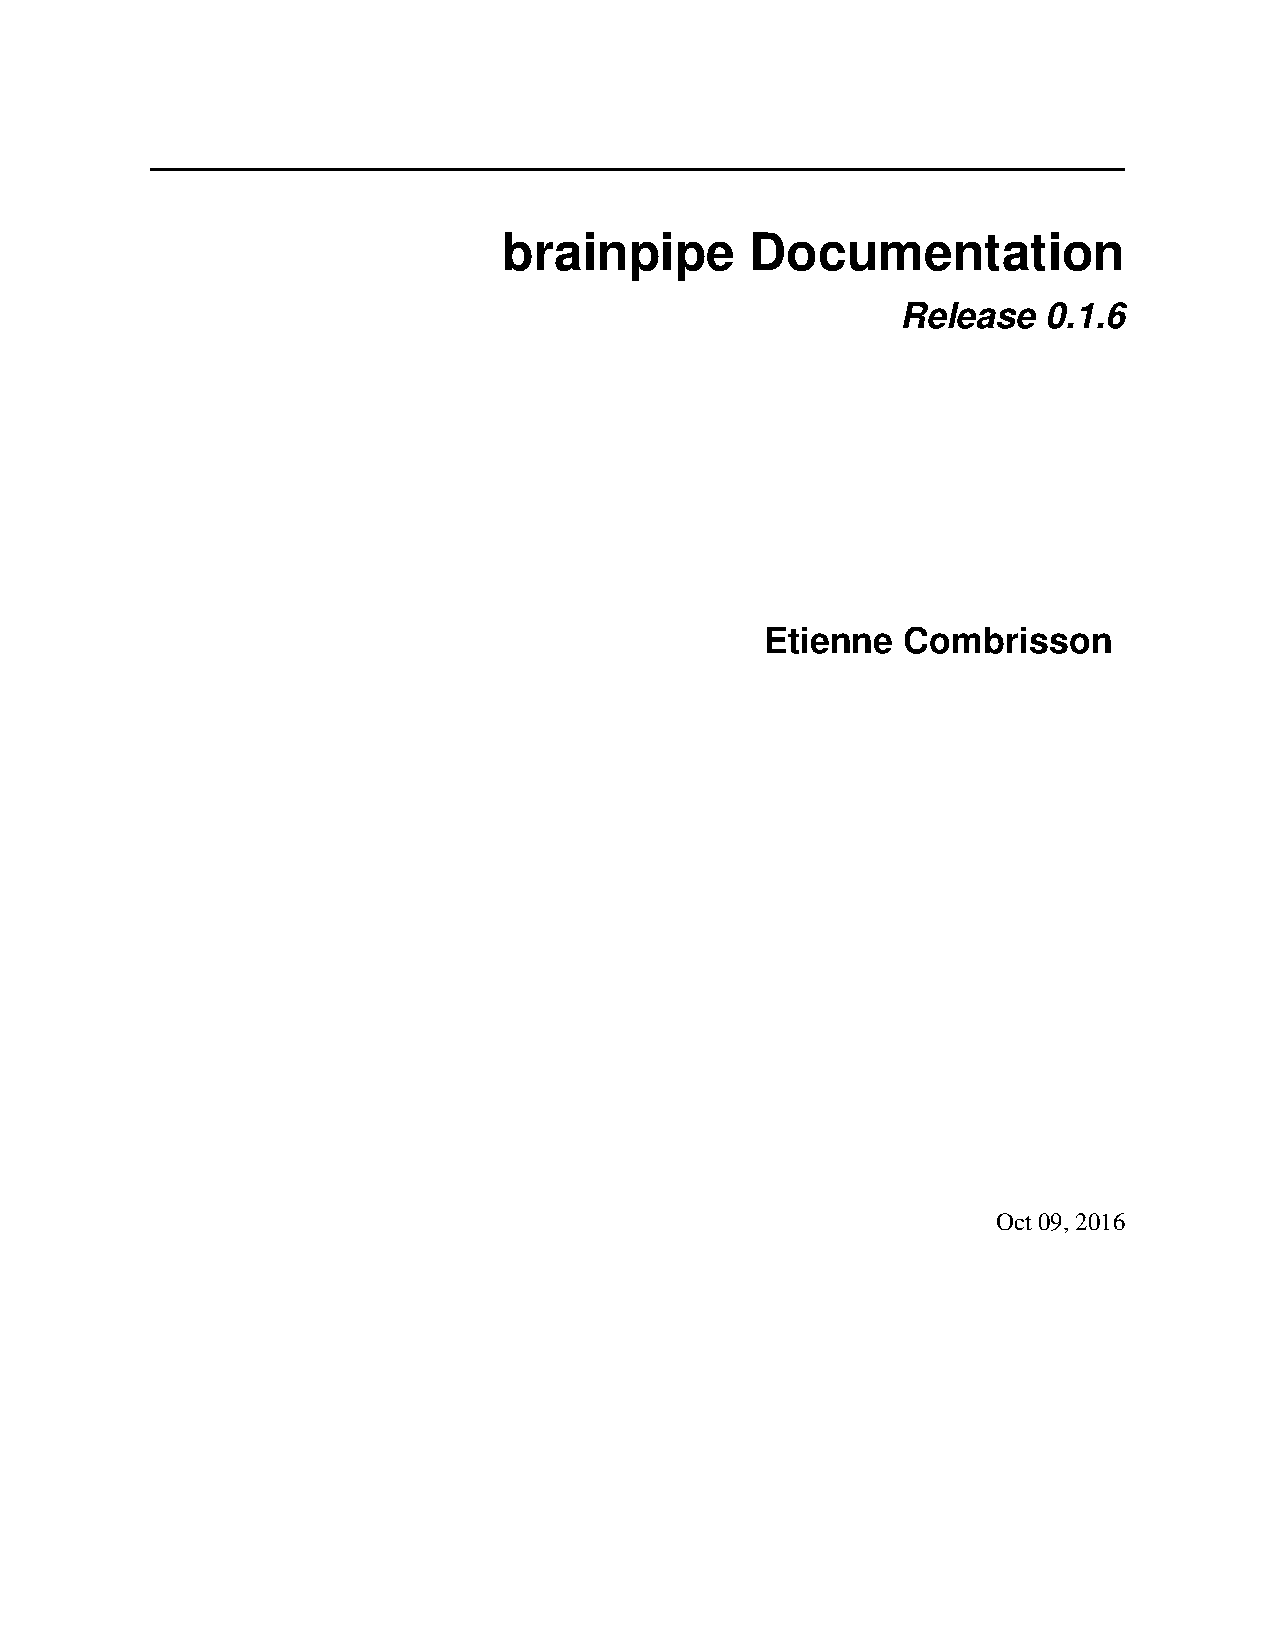
\includepdf[pages={1-69}]{Annexes/brainpipe.pdf}

}
 
% ==================================================================
% BIBLIOGRAPHIE
\makeatletter
\renewcommand*{\toclevel@chapter}{-1}
\backmatter
\bibliographystyle{apalike}
\bibliography{Manuscrit}
 
% ==================================================================
% COLOPHON
%\colophon{Ce document a �t� pr�par� � l'aide de l'�diteur de texte GNU
%  Emacs et du logiciel de composition typographique \LaTeXe.}


\end{document}
%%% Local Variables:
%%% mode: latex
%%% TeX-master: t
%%% End:
